\chapter{Appendix to Chapter 4}
\label{chap:appendix_ch4}

\section{Tuning the Initial Elliptical Slice Sampling Bracket Width}
\label{sec:lna_init_bracket_width}

When fitting SEMs with complex dynamics, e.g., when there are many strata or when the dynamics are time varying, we will be able improve the computational efficiency of our MCMC by initialing the ElliptSS bracket width at $ \omega < 2\pi $. This choice is motivated by the observation that when the model dynamics are complex, the ElliptSS bracket will typically need to be shrunk many times before the sampler reaches a range of acceptable angles in the proposal. Each time we propose a new angle in the ElliptSS algorithm we must solve the LNA ODEs in order to compute the observed data likelihood. Thus, if we can reduce the number of ElliptSS steps, we will be able to shorten the time required to complete our MCMC runs. 

In models where it is advantageous to shring the initial bracket width, we will typically set the initial bracket width to a constant times the standard deviation of the accepted angles in a tuning phase. Since we do not step out the ElliptSS bracket, the initial width should not be so small as to induce additional autocorrelation in the latent process, and should also not be so wide that the bracket is contracted needlessly. We have found a bracket width of $ \omega = 2\sqrt{2\log(10)}\sigma $, corresponding to the full width at one tenth maximum for a Gaussian with standard deviation $ \sigma $, to work well in practice. Figure \ref{fig:esstuning} presents histograms of the number of contractions per ElliptSS update and the accepted angles before and after contracting the initial ElliptSS bracket width for the joint Ebola model of Section \ref{sec:lna_ebola}. In this instance, we were able to substantially reduce the number of contractions, and hence likelihood evaluations, per ElliptSS update while leaving the distribution of accepted angles essentially unchanged. We like to call this a "free lunch".

\begin{figure}[htbp]
	\centering
	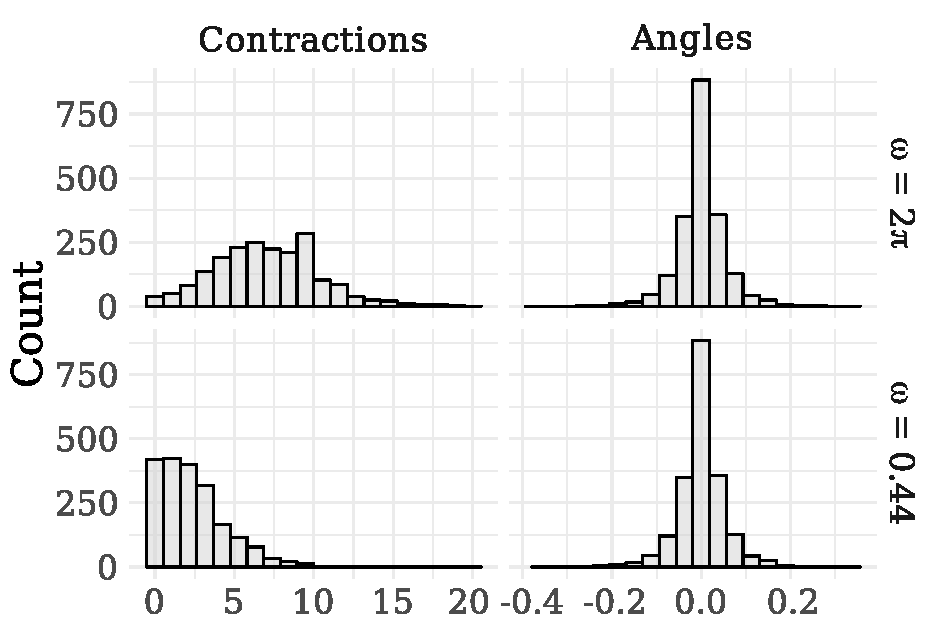
\includegraphics[width=0.7\linewidth]{figures/ess_tuning}
	\caption[Distributions of numbers of contractions and accepted for elliptical slice sampling.]{Distributions of the numbers of contractions per ElliptSS update and the accepted angles for an MCMC chain for the joint Ebola model of Section \ref{sec:lna_ebola} . An initial bracket width of $ 2\pi $ was used for the first 5,000 iterations (top row), after which the initial bracket width was set to $ 2\sqrt{2\log(10)}\sigma_{ElliptSS} $, where $ \sigma_{ElliptSS} $ was the standard deviation of the accepted angles from the initial run (bottom row).} 
	\label{fig:esstuning}
\end{figure}

We mentioned in Section \ref{subsubsec:noncentered_parameterization} that our ElliptSS algorithm was modified slightly from that presented in \cite{murray2010} in order to facilitate tuning of the initial ElliptSS bracket width. In both cases, the distribution of proposed states, $ \bZ_{prop} $, is centered at the current state $ \bZ_{cur} $. However, the distribution of angles of accepted states using our algorithm will be centered around 0, whereas the distribution of angles for accepted proposals using the algorithm in \cite{murray2010} will be bimodal with peaks at 0 and $ 2\pi $. The algorithms are nevertheless equivalent due to the rotational symmetry of the proposals (a proposal made using an angle $ \phi $ is equivalent to a proposal using $ \phi+2\pi $). It is more natural to compute the standard deviation of the accepted angles if the distribution of angles is symmetric about zero than if it is bimodal (which would require a rotation).

\section{Inference for Initial Compartment Volumes}
\label{sec:lna_init_volumes}

When the initial compartment volumes are included as initial parameters in the model instead of being treated as fixed, we will model them as arising from the following truncated multivariate normal distribution: \begin{equation}
\label{eqn:lna_initdist_prior}
\bX_0 \sim TMVN_{\mcS_X^R}(N\bp,N(\bP - \bp\bp^T)),
\end{equation} 
where $ \bp $ is a vector of subject--level initial state probabilities, $ \bP = \diag(\bp) $, $ N $ is the population size, and the subscript $ \mcS_X^R $ specifies the state space of $ \bX $ (so that the compartment volumes add up to $ N $ and each compartment volume is non--negative and less than the total population size at time $ t_0 $). Thus, the initial distribution is specified as the truncated normal approximation of a multinomial distribution with size $ N $ and probability vector $ \bp $. In models with multiple strata, we will similarly model the initial compartment volumes as having independent truncated multivariate normal distributions that are each approximations of multinomial distributions over initial compartment counts within each stratum. Notation and details are completely analogous to the single stratum case, and are therefore omitted for the sake of clarity.

Let $ \bV = N(\bP - \bp\bp^T) $, and $ \bV^{1/2} $ be the matrix square root of $ \bV $, which we will compute using the singular value decomposition $ \bV = \bU\bD\bU^T \implies \bV^{1/2} = \bU\bD^{1/2}$. Let $ \bZ^X $ denote the LNA draws as before, and let $ \bZ^{X_0}\sim\mr{MVN}(\bs{0},\mb{I}) $ denote the vector of draws that will be mapped to $ \bX_0 $. We will update the initial compartment volumes jointly with the LNA draws using elliptical slice sampling.

\begin{algorithm}[htbp]
	\caption{Sampling LNA draws and initial volumes via elliptical slice sampling.}
	\label{alg:elliptss_lna_initvols}
	\begin{algorithmic}[1]
		\Procedure{\doElliptSS2}{$ \bZ^X_{cur}, \bZ^{X_0}_{cur},\btheta,\bY,\mcI,\omega = 2\pi $}
		\State Sample ellipse: $ \bZ^X_{prop} \sim N(\bs{0}, \mb{I}),\ \bZ^{X_0}_{prop} \sim N(\bs{0}, \mb{I})$
		\State Sample threshold: $ u|\bx \sim \mr{Unif}(0, L(\bY|\doLNA(\bZ_{cur},\btheta,\mcI))) $
		\State Position the bracket and make initial proposal: \vspace{-0.1in}
		\begin{align*}
		\psi &\sim \mr{Unif}(0,\omega)\\
		L_\psi &\leftarrow -\psi;\ R_\psi \leftarrow L_\psi + \psi\\
		\phi &\sim \mr{Unif}(L_\psi,R_\psi)
		\end{align*}
		\State Set $ \bZ^{X'} \leftarrow \bZ^X_{cur}\cos(\phi) + \bZ^X_{prop}\sin(\phi) $, $ \bX_0^\prime = \bV^{1/2}\left (\bZ^{X_0}_{cur}\cos(\phi) + \bZ^{X_0}_{prop}\sin(\phi)\right ) $ 
		\If{$ L(\bY|\doLNA(\bZ',\btheta^\prime,\mcI)) > u $}{ accept $ \bZ^{X^\prime},\bZ^{X_0^\prime} $}
		\State\Return{ $ \bZ' $}
		\Else
		\State Shrink bracket and try a new angle:
		\State{\textbf{If:} $ \phi < 0 $}{ \textbf{then: }$ L_\phi \leftarrow\phi $ }{ \textbf{else: }$ R_\phi \leftarrow \phi $}
		\State $ \phi \sim \mr{Unif}(L_\phi, R_\phi) $
		\State \textbf{GoTo:} 5
		\EndIf
		\EndProcedure
	\end{algorithmic}
\end{algorithm}

\section{Choice of Estimation Scale and Implications for Mixing and Convergence}
\label{sec:est_scale_discussion}

How we parameterize the MCMC estimation scale is critically important to its computational performance. If we can identify transformations of the model parameters that minimize strong correlations and non--linear relationships on the estimation scale, we will be able to substantially improve MCMC mixing. In our context, it will often be relatively straightforward to identify such transformations (or at least intermediate transformations that can be used in combination). As a general approach, we will try to identify transformations that reflect the ways in which model parameters jointly act on the model dynamics, and then a second set of transformations that remove any boundary conditions. 
\begin{table}[htbp]
	\caption{SEIR model parameter and their interpretation on their natural scales.}
	\label{tab:seir_params_nat}
	\footnotesize
	\centering
	\begin{tabular}{clc}
		\hline
		\textbf{Parameter} & \textbf{Interpretation} & \textbf{Domain}\\
		\hline
		$\alpha$ & Rate of infectious contact from outside the population & $[ 0,\infty) $ \\
		$ \beta $ & Per--contact rate of infection within the population & $[0,\infty) $\\
		$ \omega $ & Rate of transition from $ E\rightarrow I $ & $[ 0,\infty) $\\
		$ \mu $ & Rate of transition from $ I\rightarrow R $ & $[ 0,\infty) $\\
		$ \rho $ & Mean case detection probability & $[ 0,1] $\\
		$ \phi $ & Negative binomial overdispersion parameter & $[ 0,\infty) $ \\
		$ N_{eff} $ & Effective population size & $[0,N]$\\
		\hline
	\end{tabular}
\end{table}

As an example, consider the single country SEIR model fit to the incidence data from Sierra Leone in Section \ref{sec:lna_ebola}. This model includes parameters for the external force of infection and the effective population size, which add complexity to the usual formulation of the SEIR dynamics as being entirely driven by endogenous contacts within a closed homogeneously mixing population. The effective population size is roughly the size of the initially susceptible population. The model parameters on their natural scales are provided in Table \ref{tab:seir_params_nat}. Each of the model parameters has a clear marginal interpretation, but upon examining the pairwise scatterplots of the posterior (Figure \ref{fig:slpairs1}) it becomes obvious that the parameters interact in highly non--linear ways. We would encounter a variety of pathological computational problems if we were to naively parameterize the MCMC estimation scale without considering the ways in which the parameters interact to affect the dynamics. For example, it would be extremely difficult for any sampler that does not account for the curvature in the posterior, e.g., Hamiltonian Monte Carlo (HMC), to explore the parameter space. (An aside: we experimented with implementing the LNA in \texttt{Stan} and using HMC to sample the posterior, but repeatedly integrating the LNA ODEs along with their augmented sensitivity equations was prohibitively slow for even simple models).  

\begin{figure}[htbp]
	\centering
	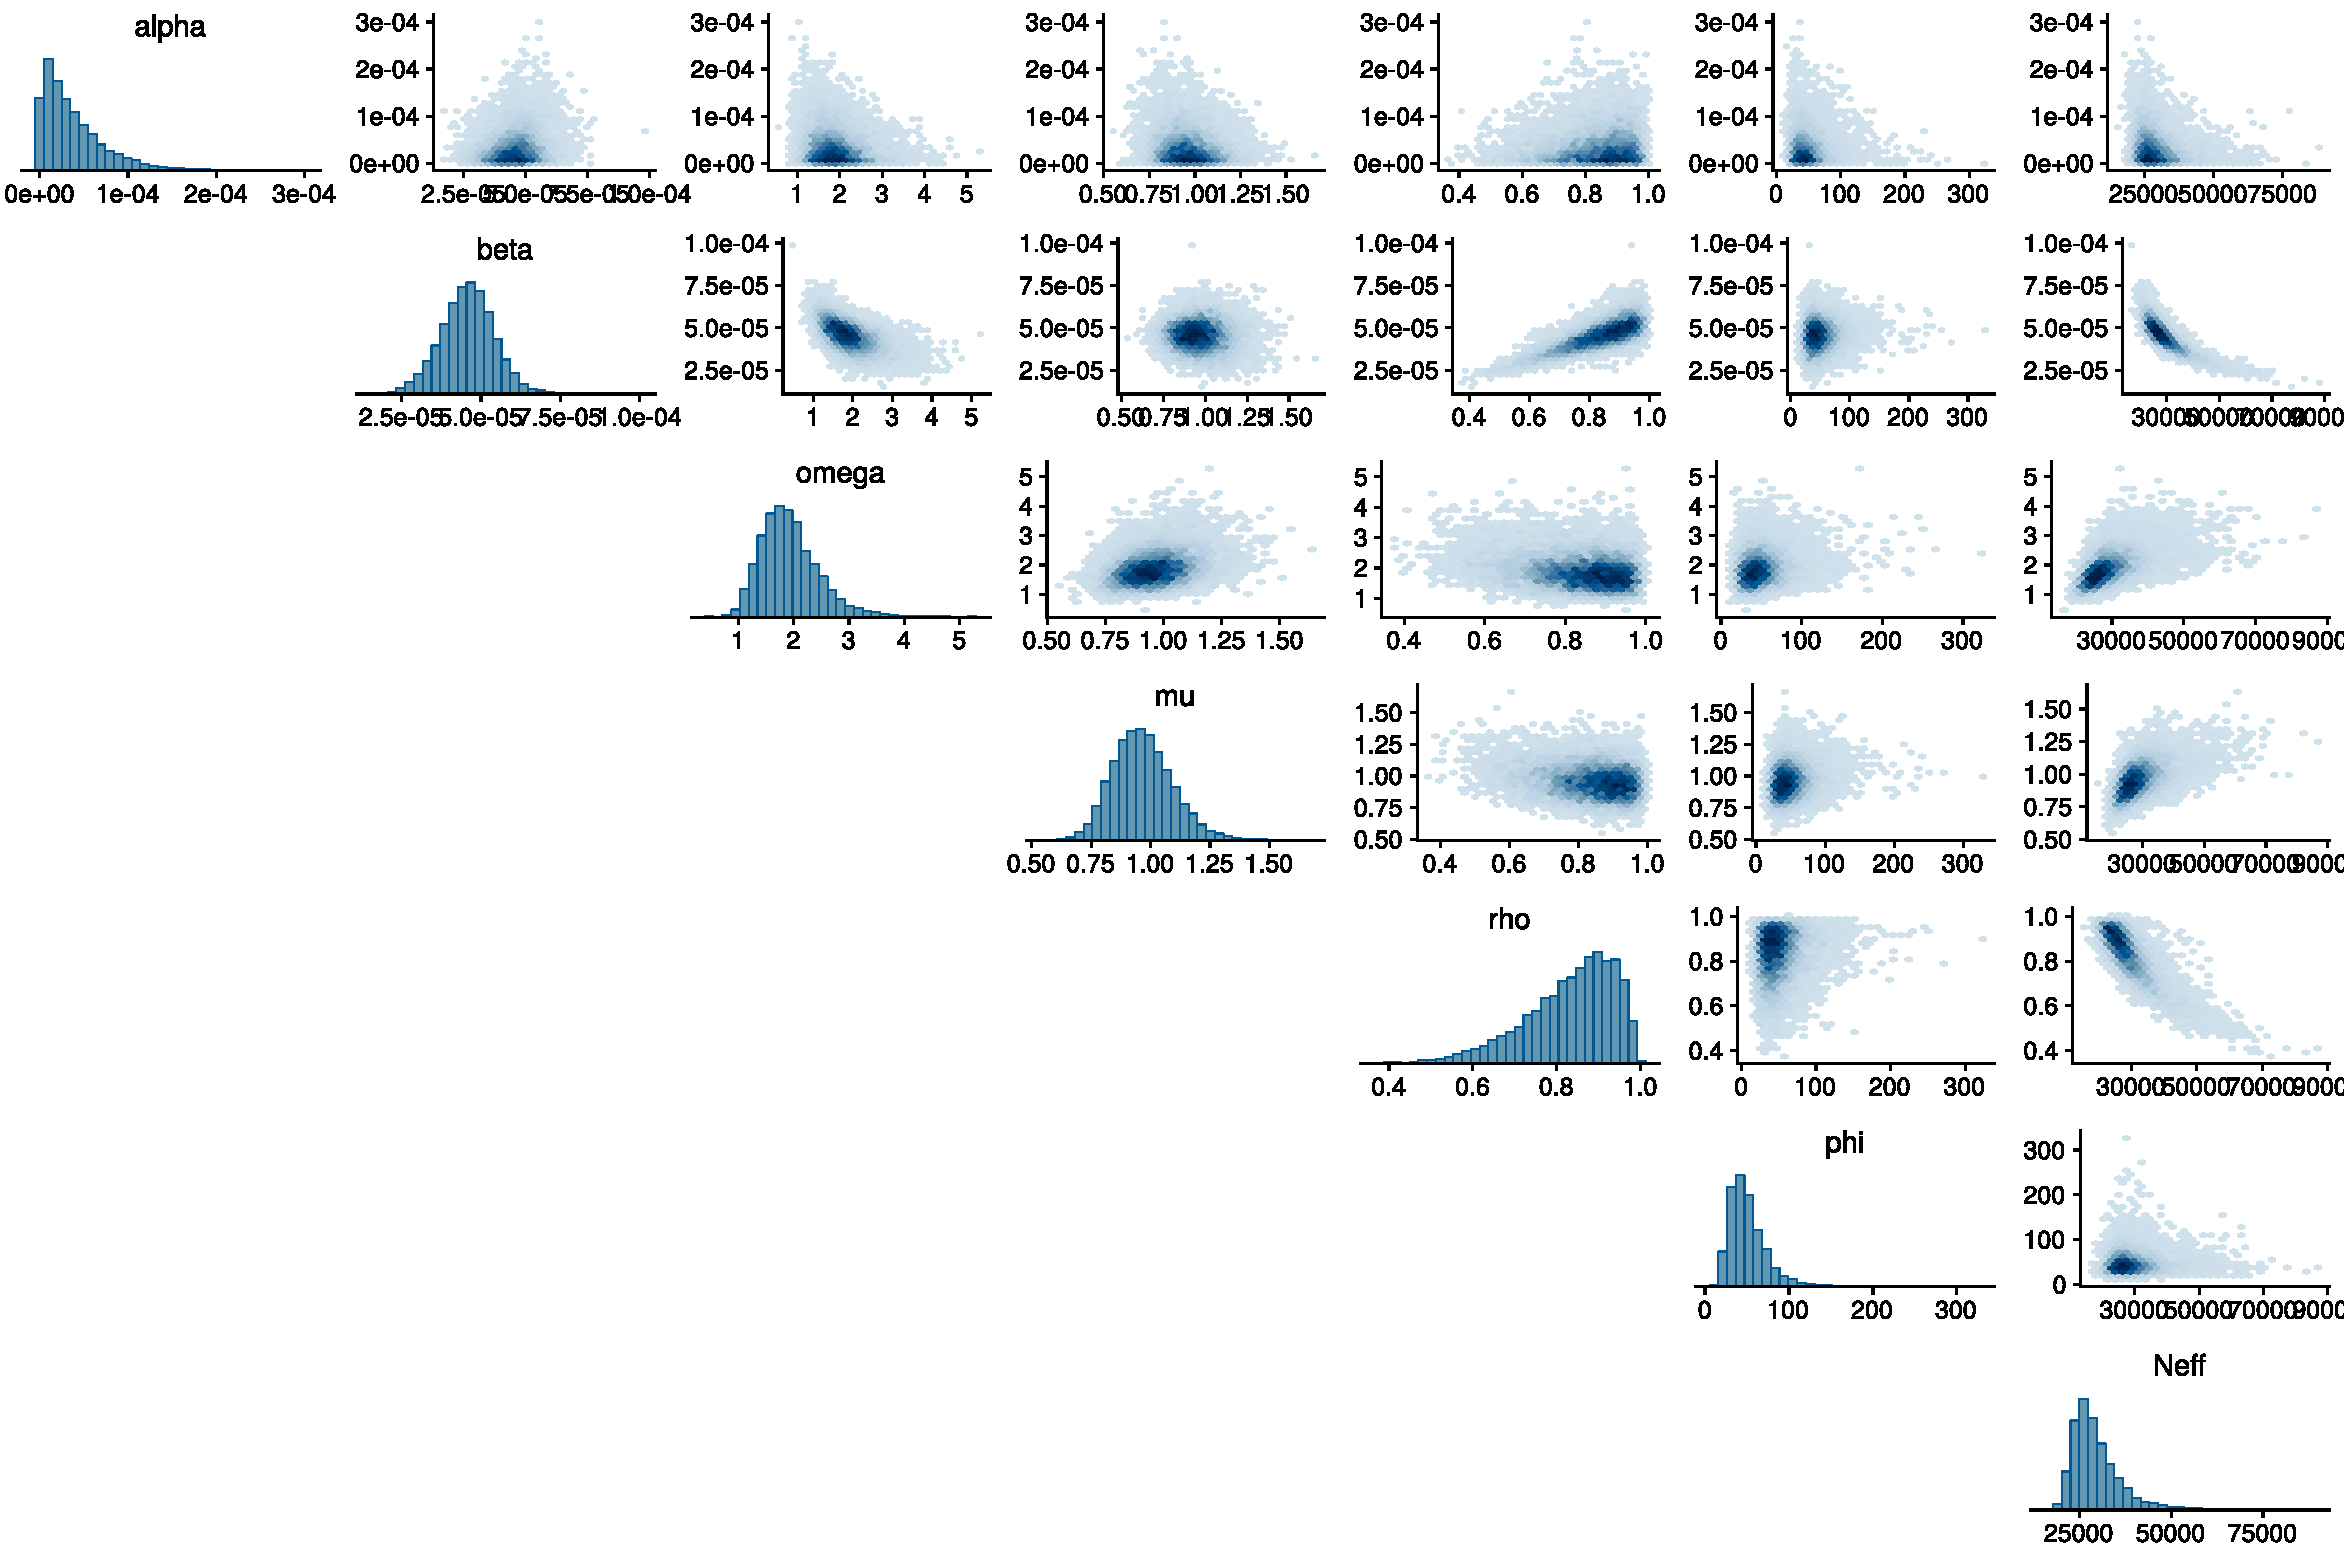
\includegraphics[width=\linewidth]{figures/sln_pairs_nat}
	\caption[Posterior scatterplots for Sierra Leone SEIR model parameters on their natural scales.]{Marginal histograms and pairwise scatterplots of posterior samples for parameters for the SEIR model fit to the Sierra Leone Ebola dataset using the estimation scale in Table \ref{tab:seir_params_est3}. The parameters on the estimation scales in this figure and their interpretations are provided in Table \ref{tab:seir_params_nat}.} 
	\label{fig:slpairs1}
\end{figure}

We can mitigate the problems caused by non--linear relationships and strong correlations among parameters by parameterizing the estimation scale in terms of how the parameters jointly affect the model dynamics and then removing the boundary conditions. Table \ref{tab:seir_params_est2} provides a list of parameters on their estimation scale that are reflective of an initial first pass at how we would expect the parameters to interact. For example, the parameters governing the rates of infectious contact, $ \alpha$ and $\beta $, combine with the effective population size and the infectious period duration to produce the basic reproductive numbers with respect to initially infected individuals outside and inside the population. Still, we can see that there are some residual non--linear relationships between the log effective population size, the logit case detection probability, and the effective reproductive number.

\begin{table}[htbp]
	\caption{SEIR model parameter and their interpretation on a possible set of estimation scales.}
	\label{tab:seir_params_est2}
	\footnotesize
	\centering
	\begin{tabular}{clc}
		\hline
		\textbf{Parameter} & \textbf{Interpretation} & \textbf{Domain}\\
		\hline
		$\log(R_{eff}^{ext}) = \log(\alpha N_{eff} / \mu)$ & \makecell[l]{Log basic reproductive number given an infected \\outside the population} & $(-\infty,\infty) $ \\
		$ \log(R_{eff} - 1) = \log(\beta N_{eff}/\mu - 1) $ & \makecell[l]{Log basic reproductive number given an infected\\ inside the population and $ R_{eff} > 1 $.} & $(-\infty,\infty) $\\
		$ \log(1/\omega) $ & Log mean latent period duration & $(-\infty,\infty) $\\
		$ \log(1/\mu) $ & Log mean infectious period duration & $ (-\infty,\infty) $\\
		$ \logit(\rho) $ & Logit mean case detection probability & $(-\infty,\infty) $\\
		$ \log(\phi) $ & Log negative binomial overdispersion parameter & $ (-\infty,\infty) $ \\
		$ \log(N_{eff}) $ & Log effective population size & $(-\infty,\log(N))$\\
		\hline
	\end{tabular}
\end{table}

\begin{figure}[htbp]
	\centering
	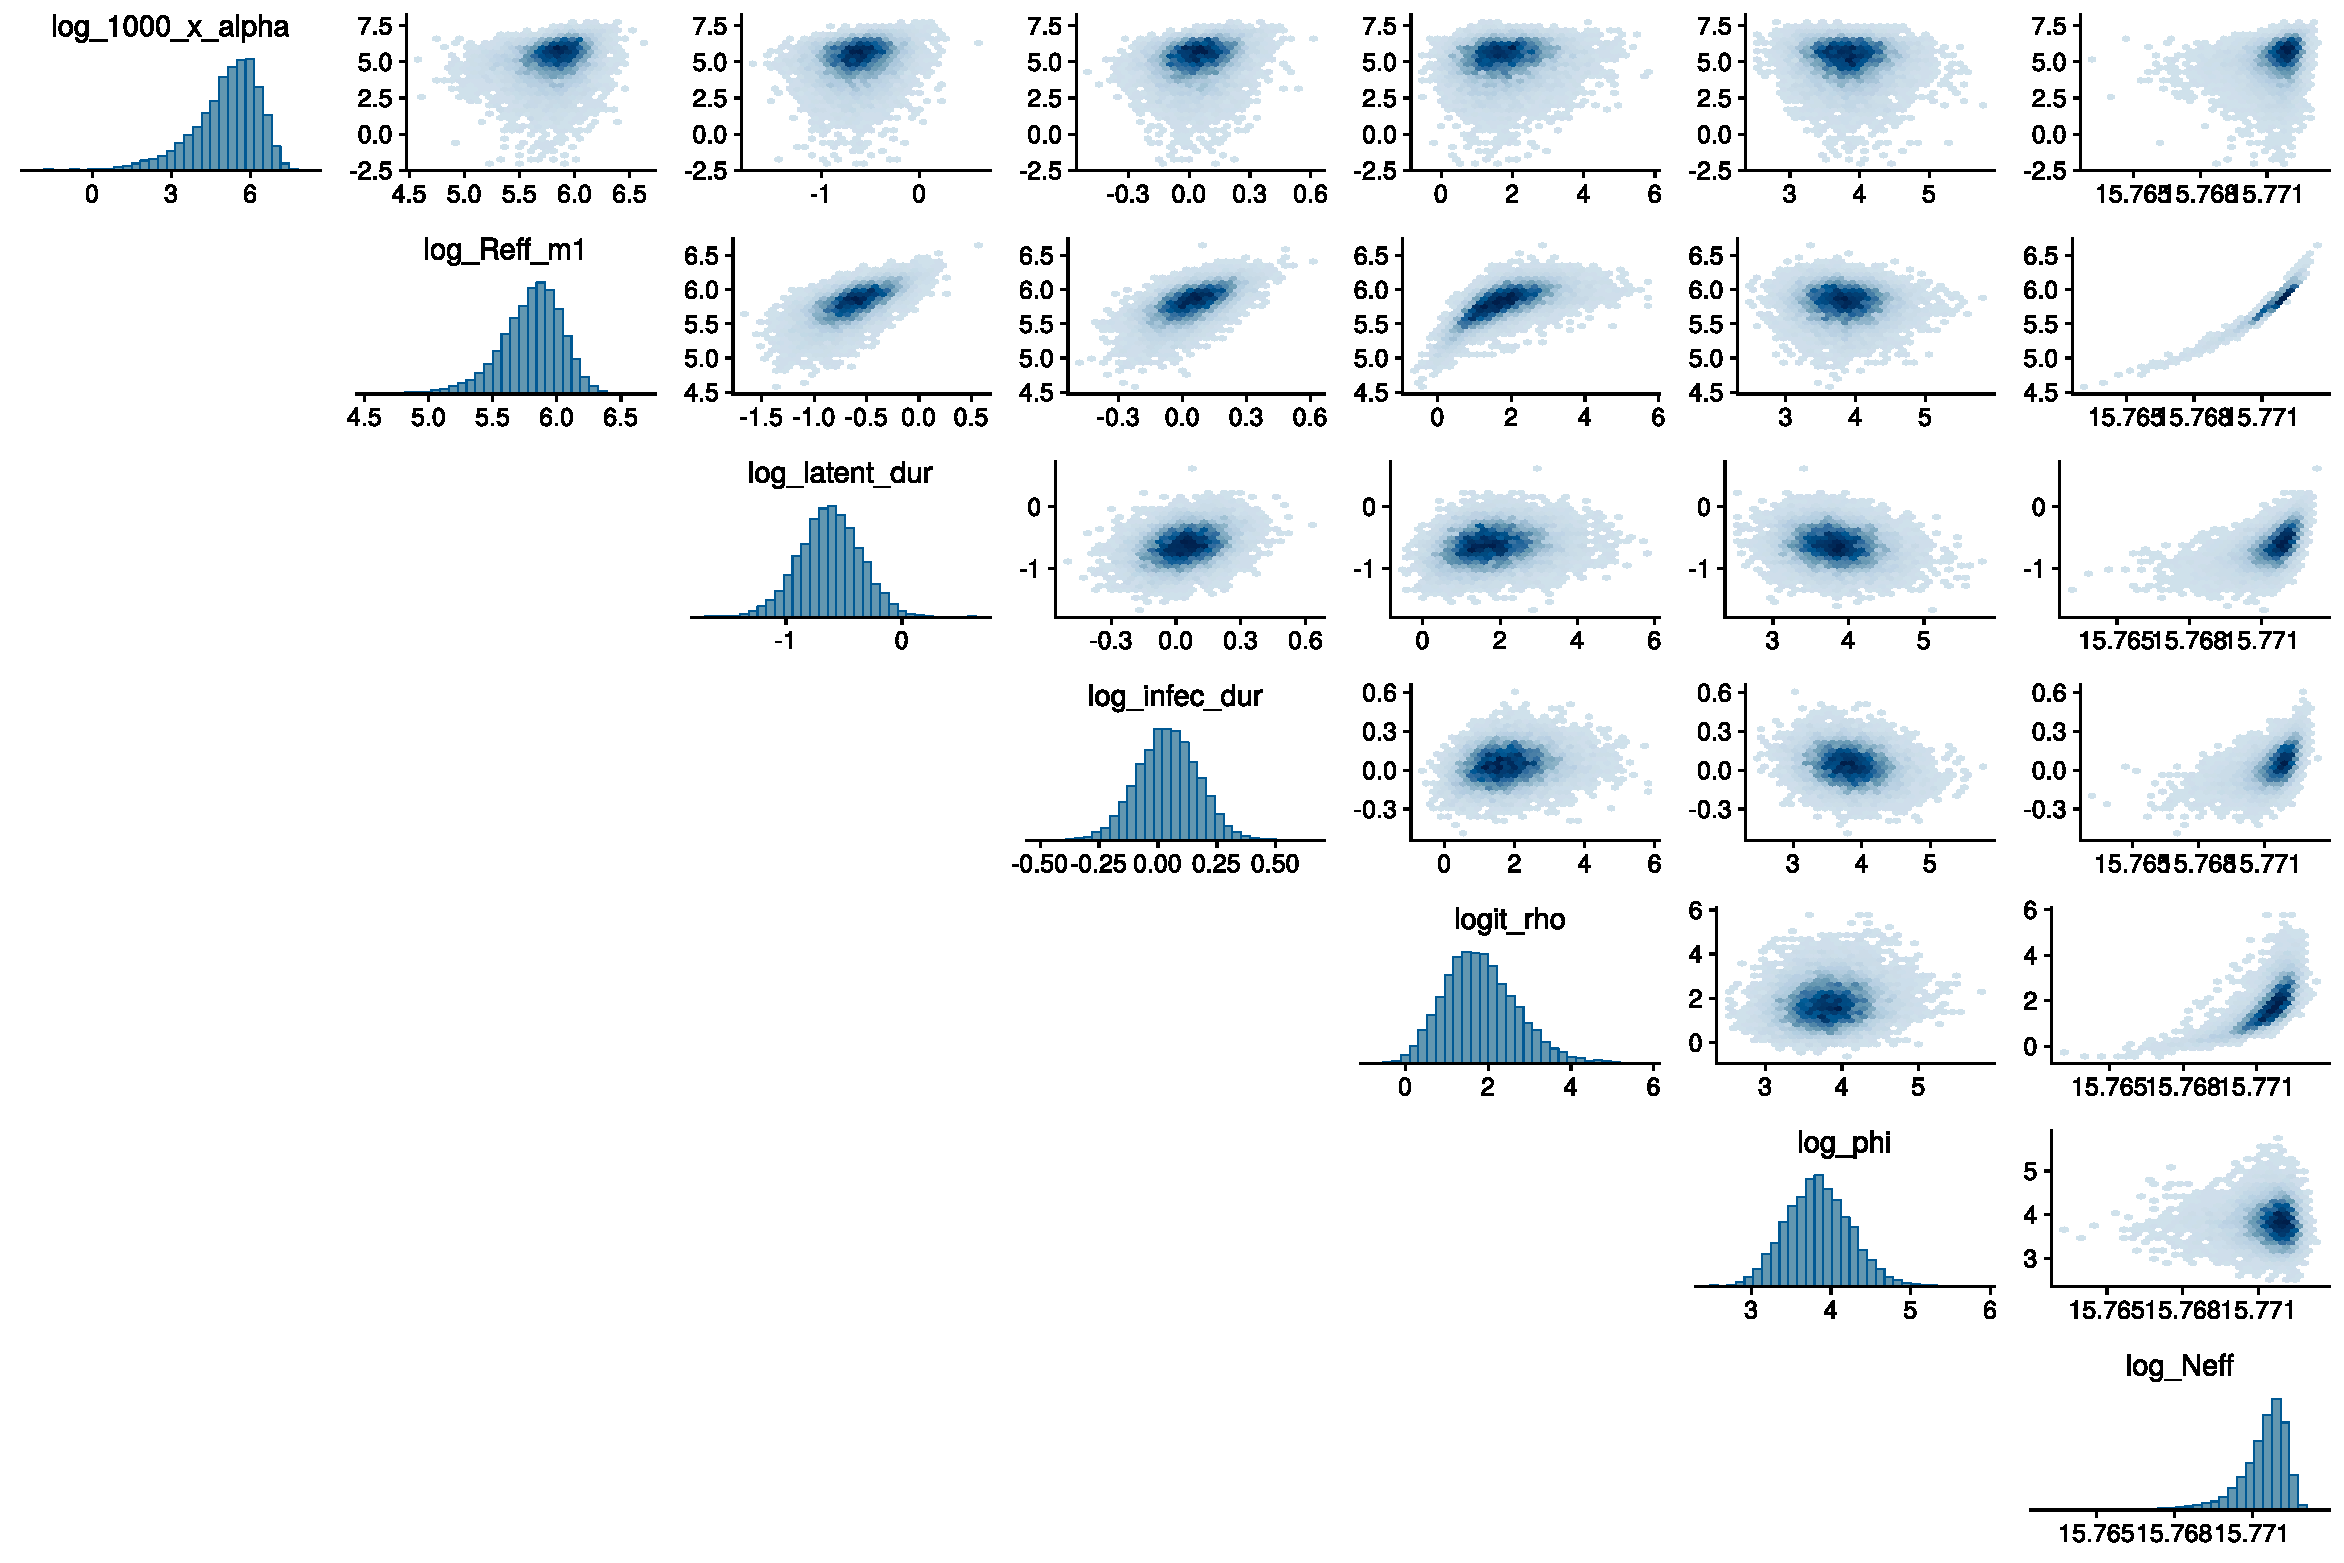
\includegraphics[width=\linewidth]{figures/sln_pairs_t1}
	\caption[Posterior scatterplots for transformed Sierra Leone SEIR model parameters.]{Marginal histograms and pairwise scatterplots of posterior samples for parameters for the SEIR model fit to the Sierra Leone Ebola dataset using the estimation scale in Table \ref{tab:seir_params_est3}. The parameters on the estimation scales in this figure and their interpretations are provided in Table \ref{tab:seir_params_est2}.} 
	\label{fig:slpairs2}
\end{figure}

A heuristic argument for an estimation scale that further simplifies the posterior geometry proceeds by analogy with the analogous deterministic ODE model. In particular, we will consider how the functions of model parameters in Table \ref{tab:seir_params_est2} act on the model dynamics through the final size relation, and how they are informed by the data. The final size relation for the ODE model \cite{miller2012note} relates the fraction of the population that eventually becomes infected $ \pi $, with the basic reproductive number:
\begin{equation}
\label{eqn:final_size_relation}
\pi = 1 - \e^{-R0\pi}.
\end{equation}
As $ R0 $ increases, a larger fraction of the population becomes infected. As the effective population size, $ N_{eff}$, increases, so too does the absolute outbreak size, $ \pi \times N_{eff} $. The expected observed outbreak size is the absolute outbreak size multiplied by the mean case detection probability, $ \pi \times \rho \times N_{eff} $, which should be concordant with the total number of observed cases. We can interpret the product, $ \rho \times N_{eff} $, as a measure of the case detection rate. This is discussed further in the next section. Taken together, the combination of parameters that we would expect to jointly act on the model, \textit{a posteriori}, is the effective reproduction number offset by the case detection rate, $ R0\times\rho \times N_{eff} $, which will enter our estimation scale as $ \log(R0\times\rho\times N_{eff}) $. The other modification of the estimation scale in Table \ref{tab:seir_params_est2} replaces the log latent period with the log ratio of infectious to latent period durations. The new estimation scale is given in Table \ref{tab:seir_params_est3}. On this estimation scale, the posterior for Sierra Leone is much better behaved, with weaker pairwise correlations and little in the way of non--linear relationships between the model parameters. 

\begin{table}[htbp]
	\caption{SEIR model parameters and their interpretation on a possible set of estimation scales.}
	\label{tab:seir_params_est3}
	\footnotesize
	\centering
	\begin{tabular}{clc}
		\hline
		\textbf{Parameter} & \textbf{Interpretation} & \textbf{Domain}\\
		\hline
		$\log(1000\alpha)$ & \makecell[l]{Log effective number of additional infecteds per \\ 1000 infecteds outside the population} & $(-\infty,\infty) $ \\
		$ \log(R_{eff} - 1) + \log(\rho N_{eff}) $ & \makecell[l]{Log basic reproductive number given an infected\\ inside the population and $ R_{eff} > 1 $, offset\\ by the mean case detection rate} & $(-\infty,\infty) $\\
		$ \log(\omega/\mu) $ & Log ratio of mean latent to infectious period durations & $(-\infty,\infty) $\\
		$ \log(1/\mu) $ & Log mean infectious period duration & $ (-\infty,\infty) $\\
		$ \logit(\rho) $ & Logit mean case detection probability & $(-\infty,\infty) $\\
		$ \log(\phi) $ & Log negative binomial overdispersion parameter & $ (-\infty,\infty) $ \\
		$ \log(\rho N_{eff}) $ & Log mean case detection rate & $(-\infty,\log(N))$\\
		\hline
	\end{tabular}
\end{table}

\begin{figure}[htbp]
	\centering
	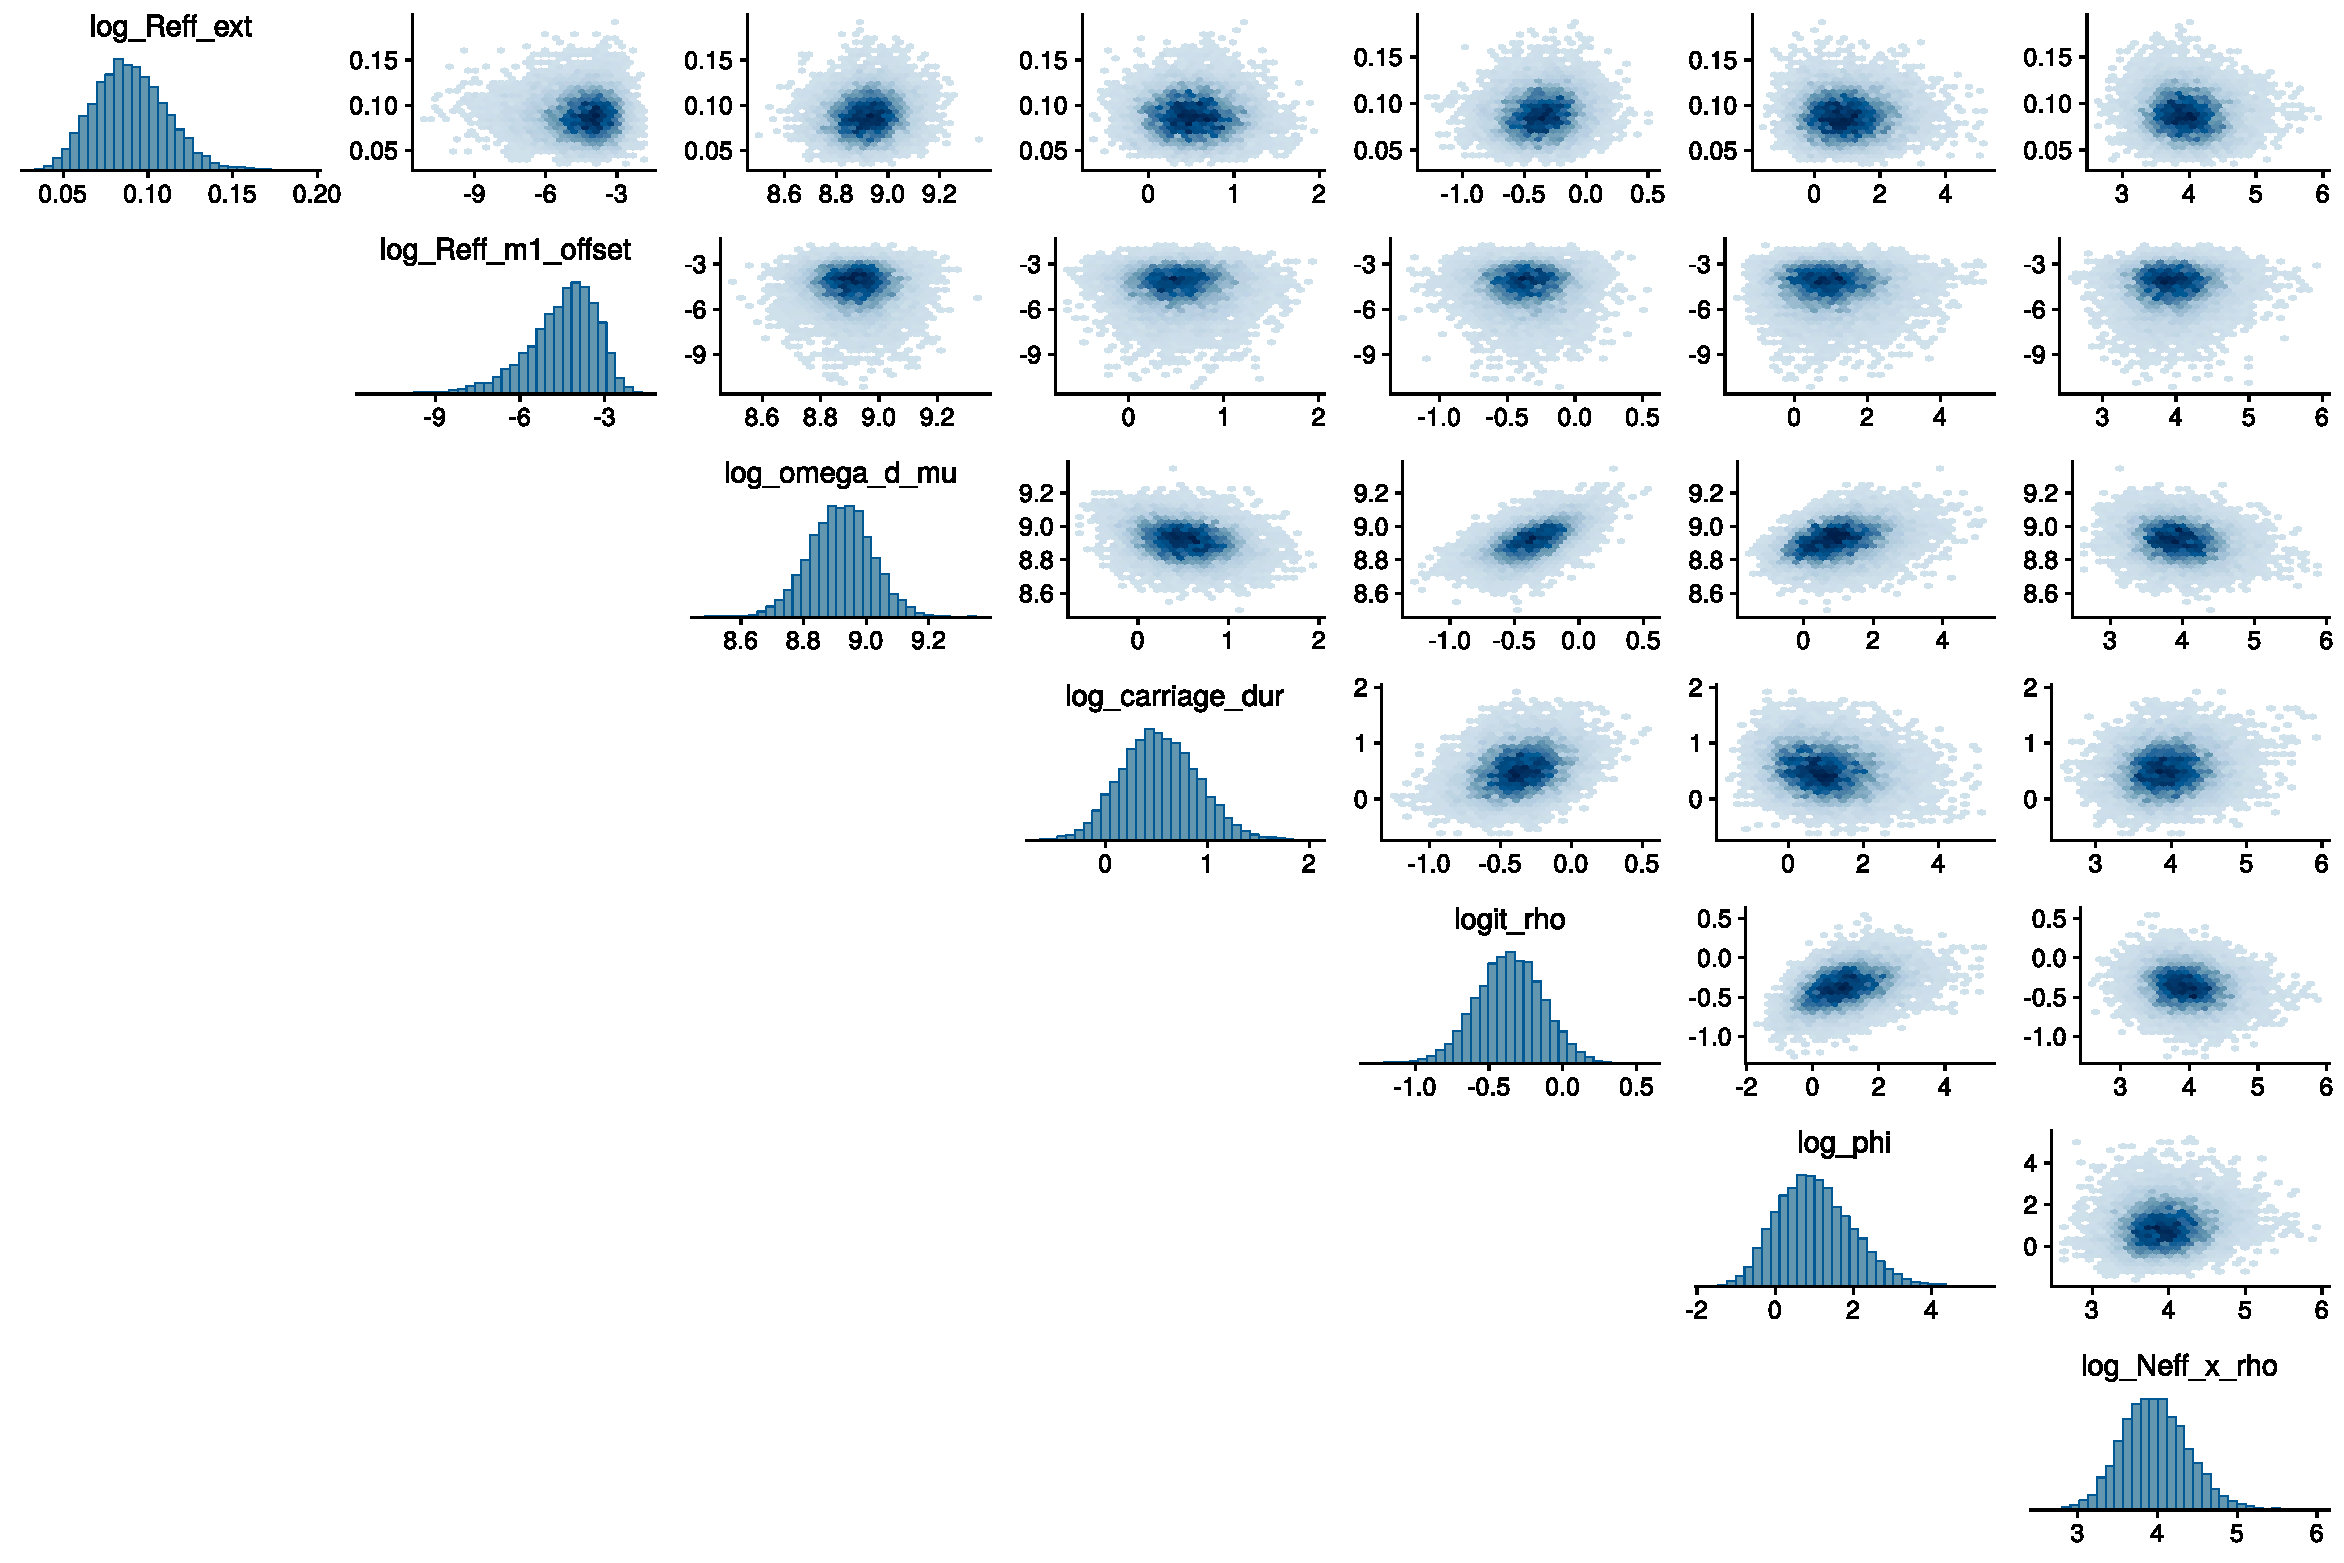
\includegraphics[width=\linewidth]{figures/sln_pairs_t2}
	\caption[Posterior scatterplots for linear combinations of transformed Sierra Leone SEIR model parameters.]{Marginal histograms and pairwise scatterplots of posterior samples for parameters for the SEIR model fit to the Sierra Leone Ebola dataset using the estimation scale in Table \ref{tab:seir_params_est3}. The parameters on the estimation scales in this figure and their interpretations are provided in Table \ref{tab:seir_params_est3}.} 
	\label{fig:slpairs3}
\end{figure}

\newpage
\section{Identifiability when Estimating the Effective Population Size}
\label{sec:effpop_identifiability}
When the scale of an outbreak is small relative to the population size, it may be unreasonable to assume that the entire population mixes homogeneously and participates in propagating the epidemic. One alternative is to split the population into two (or more) sub--populations, one that participates in the outbreak and another that is separated from the outbreak. For example, in the case of the SIR model, we might have two susceptible compartments, $ S^R $ and $ S^E $, where $ S^R $ is a susceptible subpopulation that is effectively removed since they experience no infectious contact, and $ S^E $ is a susceptible population that may become exposed. In this model, the \textit{effective population size} is $ N_{eff} = S^E + I + R $. The model is otherwise constructed in the same way as the SIR model, except with $ S^E $ replacing $ S $. 

The effective population size and the mean case detection probability are weakly identifiable parameters in that we require prior information about their scales to disentangle their effects. To see why this is so, note that $ \rho $ and $ N_{eff} $ enter into the complete data likelihood, (\ref{eqn:lna_ncp}), through the priors and through emission distributions that have means of the form, $ \rho\Delta N_{SI}(t_\ell) $. The incidence here should be understood as an increment in compartment concentrations scaled by the effective population size, since the LNA is a density dependent process \cite{komorowski2009,wilkinson2011stochastic,fearnhead2014}. Thus, the emission densities have means of the form, $ \rho\left (N^\prime_{S^SI}(t_{\ell}) - N^\prime_{S^SI}(t_{\ell-1})\right )N_{eff} $, where $ \bN^\prime = \bN/N_{eff} $ is the equivalent representation of the LNA in terms of compartment concentrations. 

In principle, absent prior information about the scales of $ \rho $ and $ N_{eff} $, we will have difficulty estimating the case detection probability and effective population size. In practice, there are a few reasons that $ \rho $ and $ N_{eff} $ might be weakly identifiable, rather than completely unidentifiable. First, certain stochastic aspects of the outbreak, such as the probability of a major outbreak and persistence of transmission, depend on the population size. Furthermore, the scale of the observed incidence and the observed outbreak duration are informative about the minimal effective population size. Therefore, the fact that we observe part of the outbreak is itself informative. Finally, a rough estimate the true population size is typically available, providing an upper bound on the effective population size. By extension, the latent epidemic process is also weakly identifiable in models where the effective population size and case detection probability are estimated.

In contrast, the mean case reporting rate, $ \rho\times N_{eff} $, along with parameters governing the outbreak dynamics, are directly informed by the data and remain identifiable. It might seem paradoxical that we can infer the dynamics of an outbreak when we are unable to estimate the latent process. To understand why this is so, note that a SEM can be rewritten in terms of concentrations by dividing the compartment counts by the population size, yielding the so--called ``true mass--action model". The dynamics of this equivalent model, expressed, for example, by the basic reproductive number $ R0 $ and recovery rate for an SIR model, are known to be independent of the population size \cite{dejong1995does}. Combinations of model parameters yield latent paths, $ \bN^\prime $, expressed in terms of increments in concentrations, and are weighted in the posterior proportionally (modulo the prior) to the likelihood of scaled paths, $ \rho N_{eff}\bN^\prime $. The temporal nature of the data is important here because the curvature of scaled paths should roughly match that of the data. Thus, we are leveraging curvature in the data to make inferences, not just the pointwise emission probabilities. 

We can check that $ \rho\times N_{eff} $ and the parameters governing the outbreak dynamics are identifiable via a simple simulation. We drew 500 sets of parameters from the priors given in Table \ref{tab:effpop_coverage_settings}, and simulated an outbreak and a dataset for each set of parameters. The models were fit via the LNA under the same priors from which the parameters were drawn using the MCMC procedure used to fit models for the main coverage simulation (described in Section \ref{subsec:lna_coverage_setup_details}). The results are summarized in Table \ref{tab:effpop_coverage_results}. The nominal coverage rates for all model parameters is approximately correct. However, the relative widths of the posterior credible intervals for the case detection rate are substantially narrower than the relative widths of the credible intervals for $ \rho $ and $ N_{eff} $ vis--a--vis their prior intervals. This suggests that the data are informative about $ \rho\times N_{eff} $. The priors for $ \rho $ and $ N_{eff} $ are not completely flat, and the scale of the observed counts is itself informative about $ N_{eff} $. Therefore, we still expect, and observe, some shrinkage for $ \rho $ and $ N_{eff} $, individually.

\begin{table}[htbp]
	\caption[Parameters and priors for a coverage simulation when estimating the effective population size.]{Parameters and priors used in simulating 500 SIR outbreaks where the effective population size was a parameter in the model. The true population size was 100,000. Each outbreak was simulated from a MJP with SIR dynamics. The observed incidence was a negative binomial sample of the true incidence.}
	\label{tab:effpop_coverage_settings}
	\small\centering
	\begin{tabular}{cllr}
		\hline
		\textbf{Parameter} & \textbf{Interpretation} & \textbf{Prior} & \textbf{Median (95\% Interval)} \\ \hline
		$ R0-1 $ & Basic reproduction \# - 1 & LogNormal(0, 0.5) & $ \implies R0 = $ 2.00 (1.38, 3.66) \\ 
		$ 1/\mu $ & Mean infectious period & LogNormal(0.7, 0.35)& 2.01 (1.01, 4.00) \\
		$ \rho / (1-\rho) $ & Odds of case detection & LogNormal(0, 1.4) & $ \implies \rho =$ 0.5 (0.06, 0.94) \\
		$ \phi $ & Neg.Binom. overdispersion & Exponential(0.1) & 6.93 (0.25, 36.89)\\
		$ N_{eff} $ & Effective population size & Unif(5000, 50000) & 27500 (6125, 48875)\\
		\hline
	\end{tabular}
\end{table}

\begin{table}[htbp]
	\caption[Coverage simulation results when estimating the effective population size]{Results for the models fit to the outbreaks simulated under SIR dynamics with random effective population sizes. Reported are the nominal coverage rates of 95\% credible intervals, the median (95\% CI) of the posterior median deviations (PMD), credible interval widths (CIW), and credible interval widths relative to the 95\% prior interval widths (Rel.CIW). The relative widths of the credible intervals for $ \rho\times N_{eff} $ are computed with respect to the induced prior resulting from the marginal priors for $ \rho $ and $ N_{eff} $.}
	\label{tab:effpop_coverage_results}
	\centering
	\small
	\begin{tabular}{ccccc}
		\hline
		\textbf{Parameter} & \textbf{Coverage} & \textbf{PMD} & \textbf{CIW} & \textbf{Rel.CIW} \\ 
		 \hline
		$ R0 $ & 0.94 & -0.02 (-0.9, 0.58) & 1.1 (0.47, 2.43) & 0.48 (0.21, 1.06) \\ 
		$ \mu $ & 0.95 & 0 (-0.36, 0.21) & 0.49 (0.29, 0.85) & 0.66 (0.4, 1.16) \\ 
		$ \rho $ & 0.95 & -0.01 (-0.36, 0.24) & 0.55 (0.14, 0.74) & 0.62 (0.16, 0.84) \\ 
		$ N_{eff} $ & 0.96 & 800 (-18900, 16100) & 32200 (14600, 41100) & 0.75 (0.34, 0.96) \\ 
		$ \rho\times N_{eff} $& 0.93 & 35 (-9000, 4200) & 6750 (640, 26750) & 0.18 (0.02, 0.72) \\ 
		$ \phi $ & 0.95 & 0.04 (-13.49, 8.95) & 9.1 (0.31, 46.85) & 0.25 (0.01, 1.28) \\ 
		\hline
	\end{tabular}
\end{table}

\newpage
\section{Simulation Details and Additional Results for Section \ref{subsec:lna_coverage}}
\label{sec:lna_coverage_supplement}

\subsection{Simulation Setup and MCMC Details}
\label{subsec:lna_coverage_setup_details}

In this simulation, repeated for each of the three different regimes of population size and initial conditions given in Table \ref{tab:lna_coverage_sim}, we simulated 500 datasets according to the following procedure:
\begin{enumerate}
	\item Draw $ \log(R0 - 1),\ 1/\mu,\ \logit(\rho),\ \log(\phi) $ from the priors given in Table \ref{tab:lna_coverage_sim}.
	\item Simulate an outbreak, $ \bN|\btheta $, under SIR dynamics from the MJP via Gillespie's direct algorithm \cite{gillespie1976general}. If there were fewer than 15 cases, simulate another outbreak. 
	\item Simulate the observed incidence, $ \bY|\bN,\btheta $, as a negative binomial sample of the true incidence in each epoch, i.e., $ Y_\ell\sim\mr{Neg.Binomial(\rho(N_{SI}(t_\ell) - N_{SI}(t_{\ell-1})), \phi)} $. If the outbreak died off before epoch 15, the dataset was truncated at 15 observations (i.e., the dataset consisted of a series of case counts accrued during the outbreak along with a series of trailing zeros accrued after the outbreak died off). If the outbreak lasted longer than 50 epochs, the dataset was truncated at 50 observations
\end{enumerate}

We proceed to fit SIR models using the LNA, ODE, and MMTL approximations. Priors for model parameters were assigned as in Table \ref{tab:lna_coverage_sim}. Five MCMC chains per model were initialized at random values near the true parameters and run for 35,000 iterations per chain. The first 10,000 iterations used to warm up each chain and adaptively estimate the empirical covariance matrix to be used in the multivariate Gaussian random walk Metropolis--Hastings proposals for parameters. The empirical covariance matrix was initialized as 0.01 times an identity matrix. After the warm--up period, the empirical covariance matrix was frozen and the final 25,000 iterations from each chain were combined to form the final MCMC sample. Convergence was assessed using potential scale reduction factors (PSRFs) \cite{brooks1998general}, computed via the \texttt{coda} R package \cite{codapackage}. PSRFs were less than 1.05 in all cases.

For models fit via the LNA and ODE approximations, the covariance matrix was adapted as in algorithm 4 of \cite{andrieu2008tutorial}. The gain factor sequence was $\gamma_n = 0.25(1 + 0.05n)^{-0.50001}$, and a small nugget variance, equal to 0.00001 times an identity matrix, was added during the adaptation phase. The target acceptance rate used in the adaptation was 0.234. The models were implemented using the \text{stemr} R package \cite{stemr}.

Inference via the MMTL approximation within PMMH were fit using the \texttt{pomp} R package \cite{pompjss}. We used 500 particles in the PMMH algorithm. This choice was made to mitigate issues of particle degeneracy that occurred with fewer particles for some datasets. The time step for MMTL was set to 1/7, which, for example, corresponds to $ \tau $--leaping over one day increments given weekly incidence data. The MCMC was initialized in the same way as LNA and ODE models, but the empirical covariance matrix was adapted according to a different cooling schedule. The gain factor sequence provided by the package is of the form $ \gamma_n = n^\alpha $, where the cooling term, $ \alpha $, was set to 0.999. For some of the datasets, the PMMH algorithm degenerated during the adaptive phase of the MCMC. If this was the case, the MCMC was restarted at a different set of random initial conditions. The posterior samples from all five MCMC chains were combined after discarding the initial samples from the adaptation phase.

\newpage
\subsection{Additional Coverage Simulation Results}
\label{subsec:lna_coverage_additional_results}

\begin{table}[htbp]
	\small
	\centering
	\begin{tabular}{lccc}
		\hline
		\textbf{Population siz}e & \textbf{ODE} & \textbf{LNA} & \textbf{MMTL}\\ 
		\hline
		10,000 & 0.39 (0.21, 0.62) & 21.73 (10.83, 37.74) & 85.23 (42.31, 152.48) \\ 
		50,000& 0.42 (0.23, 0.62) & 32.27 (13.4, 55.8) & 88.36 (38.63, 153.54) \\ 
		250,000 & 0.45 (0.25, 0.78) & 33.08 (12.56, 70.86) & 87.4 (39.8, 166.87) \\
		\hline
	\end{tabular}
	\caption[Run times for coverage simulation SIR models fit via the LNA, ODE, and MMTL approximations.]{Median (2.5\%, 97.5\%) quantiles of run times, in minutes, for MCMC chains in the coverage simulation presented in Section \ref{subsec:lna_coverage}. Models were fit via the linear noise approximation (LNA), multinomial modified $ \tau $--leaping (MMTL) within particle marginal Metropolis--Hastings, and deterministic ordinary differential equations (ODE).}
\end{table}	

\begin{sidewaystable}[htbp]
	\begin{fullpage}
		\small
		\centering
		\begin{tabular}{lcccccc}
			\hline
			Method & Parameter & Coverage & PMD & 95\% CIW & ESS & Rel. GM ESS/CPU time \\ 
			\hline
			LNA & log(R0) & 0.93 & 0 (-0.51, 0.55) & 1.04 (0.83, 1.36) & 1340 (274, 4029) & 0.63 (0.13, 3.4) \\ 
			LNA & log($\mu$) & 0.95 & -0.01 (-0.5, 0.48) & 0.93 (0.74, 1.13) & 1024 (199, 3988) & 0.48 (0.1, 2.91) \\ 
			LNA & logit($\rho$) & 0.93 & -0.05 (-1.44, 0.56) & 1.18 (0.54, 2.86) & 1225 (316, 3941) & 0.62 (0.17, 4.05) \\ 
			LNA & log($\phi$) & 0.96 & 0 (-0.66, 0.71) & 1.35 (0.92, 2.22) & 2021 (687, 4535) & 1 (0.31, 3.53) \\ 
			MMTL & log(R0) & 0.95 & 0.03 (-0.48, 0.55) & 1.09 (0.88, 1.39) & 7483 (5453, 9197) & --- \\ 
			MMTL & log($\mu$) & 0.95 & -0.03 (-0.51, 0.45) & 0.92 (0.75, 1.09) & 7481 (5442, 9197) & --- \\ 
			MMTL & logit($\rho$) & 0.94 & -0.03 (-1, 0.61) & 1.17 (0.51, 2.98) & 6725 (4328, 8506) & --- \\ 
			MMTL & log($\phi$) & 0.96 & -0.02 (-0.69, 0.71) & 1.33 (0.91, 2.21) & 7486 (5405, 9215) & --- \\ 
			ODE & log(R0) & 0.89 & -0.03 (-0.76, 0.56) & 1.03 (0.65, 1.38) & 6438 (4956, 7650) & 185 (105, 340) \\ 
			ODE & log($\mu$) & 0.86 & 0.05 (-0.51, 0.79) & 0.91 (0.53, 1.2) & 6420 (4908, 7663) & 184 (103, 344) \\ 
			ODE & logit($\rho$) & 0.72 & 0.12 (-1.03, 1.37) & 1.25 (0.48, 2.94) & 6237 (4346, 7556) & 203 (111, 401) \\ 
			ODE & log($\phi$) & 0.75 & -0.25 (-1.64, 0.54) & 1.25 (0.88, 2.11) & 6529 (5459, 7778) & 189 (116, 340) \\ 
			\hline
		\end{tabular}
		\caption[Small population coverage results for SIR models fit via the LNA, ODE, and MMTL approximations.]{Detailed small population (N = 10,000) regime results for the coverage simulation presented in Section \ref{subsec:lna_coverage}. Models were fit via the linear noise approximation (LNA), multinomial modified $ \tau $--leaping (MMTL) within particle marginal Metropolis--Hastings, and deterministic ordinary differential equations (ODE). $ R_0 $ is the basic reproductive number of an outbreak, $ \mu $ is the recovery rate, $ \rho $ is the negative binomial case detection probability, $ \phi $ is the negative binomial over--dispersion parameter. We report the coverage rates of 95\% Bayesian credible intervals along with 50\% (2.5\%, 97.5\%) quantiles of posterior median deviations (PMD), 95\% credible interval widths (CIW), effective sample size (ESS), and relative geometric mean effective sample size per CPU time (Rel. GM ESS/CPU time).}
	\end{fullpage}
\end{sidewaystable}	

\begin{sidewaystable}[htbp]
	\begin{fullpage}
		\small
		\centering
		\begin{tabular}{lcccccc}
			\hline
			Method & Parameter & Coverage & PMD & 95\% CIW & ESS & Rel. GM ESS/CPU time \\ 
			\hline
			LNA & log(R0) & 0.93 & -0.03 (-0.5, 0.49) & 0.93 (0.66, 1.28) & 2158 (397, 4981) & 0.67 (0.16, 3) \\ 
			LNA & log($\mu$) & 0.93 & 0.01 (-0.43, 0.41) & 0.83 (0.58, 1.07) & 1919 (307, 5276) & 0.63 (0.12, 3.05) \\ 
			LNA & logit($\rho$) & 0.95 & -0.01 (-1, 0.5) & 1.13 (0.47, 2.81) & 1704 (439, 4636) & 0.61 (0.18, 3.49) \\ 
			LNA & log($\phi$) & 0.94 & 0.01 (-0.57, 0.7) & 1.1 (0.79, 1.86) & 2916 (1179, 5442) & 1.02 (0.38, 3.1) \\ 
			MMTL & log(R0) & 0.95 & -0.01 (-0.46, 0.51) & 0.98 (0.67, 1.32) & 7284 (4713, 9107) & --- \\ 
			MMTL & log($\mu$) & 0.93 & -0.01 (-0.47, 0.37) & 0.82 (0.58, 1.05) & 7167 (4488, 8912) & --- \\ 
			MMTL & logit($\rho$) & 0.95 & -0.03 (-0.98, 0.56) & 1.09 (0.43, 2.96) & 6452 (3999, 8318) & --- \\ 
			MMTL & log($\phi$) & 0.94 & -0.02 (-0.59, 0.65) & 1.1 (0.79, 1.84) & 7096 (4640, 8999) & --- \\ 
			ODE & log(R0) & 0.86 & -0.02 (-0.56, 0.59) & 0.84 (0.52, 1.27) & 6592 (5213, 7771) & 187 (88, 354) \\ 
			ODE & log($\mu$) & 0.82 & -0.01 (-0.66, 0.47) & 0.73 (0.44, 1.07) & 6558 (5129, 7664) & 190 (87, 359) \\ 
			ODE & logit($\rho$) & 0.75 & -0.03 (-1.13, 0.85) & 0.88 (0.37, 2.75) & 6421 (5017, 7643) & 209 (107, 410) \\ 
			ODE & log($\phi$) & 0.82 & -0.17 (-1.36, 0.57) & 1.04 (0.78, 1.7) & 6637 (5452, 7755) & 193 (102, 365) \\ 
			\hline
		\end{tabular}
		\caption[Medium population coverage results for SIR models fit via the LNA, ODE, and MMTL approximations.]{Detailed medium population (N = 50,000) regime results for the coverage simulation presented in Section \ref{subsec:lna_coverage}. Models were fit via the linear noise approximation (LNA), multinomial modified $ \tau $--leaping (MMTL) within particle marginal Metropolis--Hastings, and deterministic ordinary differential equations (ODE). $ R_0 $ is the basic reproductive number of an outbreak, $ \mu $ is the recovery rate, $ \rho $ is the negative binomial case detection probability, $ \phi $ is the negative binomial over--dispersion parameter. We report the coverage rates of 95\% Bayesian credible intervals along with 50\% (2.5\%, 97.5\%) quantiles of posterior median deviations (PMD), 95\% credible interval widths (CIW), effective sample size (ESS), and relative geometric mean effective sample size per CPU time (Rel. GM ESS/CPU time).}
	\end{fullpage}
\end{sidewaystable}	

\begin{sidewaystable}[htbp]
	\begin{fullpage}
		\small
		\centering
		\begin{tabular}{lcccccc}
			\hline
			Method & Parameter & Coverage & PMD & 95\% CIW & ESS & Rel. GM ESS/CPU time \\ 
			\hline
			LNA & log(R0) & 0.95 & -0.01 (-0.38, 0.51) & 0.77 (0.47, 1.24) & 3248 (638, 6127) & 1.13 (0.22, 3.99) \\ 
			LNA & log($\mu$) & 0.95 & 0.01 (-0.44, 0.33) & 0.67 (0.4, 1.02) & 3134 (499, 6038) & 1.12 (0.18, 3.95) \\ 
			LNA & logit($\rho$) & 0.93 & 0.01 (-0.8, 0.57) & 0.99 (0.35, 2.66) & 2514 (572, 5905) & 1.03 (0.24, 4.71) \\ 
			LNA & log($\phi$) & 0.95 & 0 (-0.44, 0.54) & 0.94 (0.67, 1.5) & 3987 (2201, 6184) & 1.63 (0.71, 3.95) \\ 
			MMTL & log(R0) & 0.93 & 0.03 (-0.38, 1.04) & 0.8 (0.31, 1.27) & 7030 (3789, 8915) & --- \\ 
			MMTL & log($\mu$) & 0.94 & -0.02 (-0.46, 0.32) & 0.65 (0.38, 0.98) & 6858 (3602, 8871) & --- \\ 
			MMTL & logit($\rho$) & 0.92 & 0.01 (-0.7, 0.65) & 0.95 (0.34, 2.64) & 6166 (3282, 7906) & --- \\ 
			MMTL & log($\phi$) & 0.95 & -0.03 (-0.51, 0.52) & 0.94 (0.66, 1.5) & 6266 (3735, 8960) & --- \\ 
			ODE & log(R0) & 0.89 & -0.01 (-0.37, 0.55) & 0.65 (0.36, 1.22) & 6828 (5566, 8025) & 193 (104, 417) \\ 
			ODE & log($\mu$) & 0.89 & 0 (-0.49, 0.34) & 0.55 (0.3, 1) & 6815 (5520, 7877) & 198 (105, 428) \\ 
			ODE & logit($\rho$) & 0.84 & -0.01 (-0.78, 0.68) & 0.74 (0.27, 2.62) & 6575 (5219, 7838) & 210 (118, 486) \\ 
			ODE & log($\phi$) & 0.91 & -0.08 (-0.59, 0.46) & 0.9 (0.64, 1.44) & 6721 (5571, 7683) & 209 (117, 413) \\ 
			\hline
		\end{tabular}
		\caption[Large population coverage results for SIR models fit via the LNA, ODE, and MMTL approximations.]{Detailed large population (N = 250,000) regime results for the coverage simulation presented in Section \ref{subsec:lna_coverage}. Models were fit via the linear noise approximation (LNA), multinomial modified $ \tau $--leaping (MMTL) within particle marginal Metropolis--Hastings, and deterministic ordinary differential equations (ODE). $ R_0 $ is the basic reproductive number of an outbreak, $ \mu $ is the recovery rate, $ \rho $ is the negative binomial case detection probability, $ \phi $ is the negative binomial over--dispersion parameter. We report the coverage rates of 95\% Bayesian credible intervals along with 50\% (2.5\%, 97.5\%) quantiles of posterior median deviations (PMD), 95\% credible interval widths (CIW), effective sample size (ESS), and relative geometric mean effective sample size per CPU time (Rel. GM ESS/CPU time).}
	\end{fullpage}
\end{sidewaystable}	

\newpage

\section{Supplementary Coverage Simulations with Fixed Parameters}
\label{sec:lna_fixedpar_coverage}

\subsection{Simulation Setup}
\label{subsec:lna_fixedpar_setup}

The simulations presented in this section supplement the results of Section \ref{subsec:lna_coverage} in assessing the statistical and computation performance of the LNA approximation vis--a--vis the ODE and MMTL approximations. In contrast to the previous coverage simulation, here we will fix the model parameters to one of four regimes, presented in Table \ref{tab:lna_supplementary_coverage_sim}, that are characterized by either fast or moderate outbreak dynamics, and high or low detection probability. In each setting, we simulated 500 outbreaks from a MJP with SIR dynamics in a population of 50,000 individuals, five of whom were initially infected and the rest of whom were susceptible. The observed incidence in each epoch was a negative binomial sample of the true incidence. Outbreaks for which the number of observed cases was less than 25 were re--simulated. MCMC chains were tuned and SIR models were fit via the LNA, ODE, and MMTL approximations as described in Section \ref{subsec:lna_coverage_setup_details}. The initial comparment volumes were fixed at the true values. The models were fit using diffuse priors, also presented in Table \ref{tab:lna_supplementary_coverage_sim}. We caution that the priors used in this exercise are perhaps unreasonably diffuse, particularly in the context of epidemic modeling where prior information is often available, and that we expect credible intervals will be overly wide as a result (we would still expect nominal coverage to be incorrect, even under tighter priors, since the datasets were simulated under fixed parameter regimes).

\newpage

\subsection{Fixed Parameter Coverage Results}
\label{subsec:lna_fixedpar_sim_results}

Coverage for credible intervals of ODE models tended to fall below nominal levels in spite of the bias towards wide intervals due to the diffusivity of the priors. This was particularly the case in parameter regimes 1 and 3, where the basic reproductive number was lower (and hence the simulated outbreak trajectories further from their thermodynamic limits). In these parameter regimes, coverage was particularly poor due as estimates of the outbreak dynamics tended to be farther from their true values and credible intervals were too tight and did not properly account for uncertainty about the parameter estimates, particularly those governing the measurement process. Coverage levels for models fit via the LNA and MMTL approximations exceeded their nominal levels as expected. 

ODE models remained the most computationally performant. However, in this exercise, the LNA substantially outperformed the MMTL approximation within PMMH in terms of ESS and ESS per CPU time. We believe this is largely attributable to the diffusivity of the priors, which not only fail to regularize the posterior, but likely pull it towards unreasonable regions of the parameter space. As a general comment, we would strongly caution practitioners against adopting such priors more broadly. While it may seem appealing to adopt such diffuse priors in pursuit of being "agnostic" to the underlying outbreak dynamics, one of the very good reasons for working within the Bayesian paradigm in this context is that we have quite a bit of prior information regarding the outbreak dynamics and reasonable ranges for the case detection probability. For example, we often have historic examples of outbreaks in similar settings that we can look to in specifying priors about the basic reproductive number.

\begin{table}[htbp]
	\caption[Fixed parameter coverage simulation setup.]{Parameter regimes under which datasets were simulated and priors used to fit SIR models. Five hundred datasets were simulated for each of the parameter regimes  from a MJP with SIR dynamics. $ R0 = \beta N / \mu $ is the basic reproductive number and $ \mu $ is the recovery rate. The observed incidence was a negative binomial sample of the true incidence in each inter--observation interval with case detection probability $ \rho $ and overdispersion parameter $ \phi $.}
	\label{tab:lna_supplementary_coverage_sim}
	\footnotesize
	\centering
	\begin{tabular}{ccccc}
		\hline
		& \textbf{Regime 1} & \textbf{Regime 2} & \textbf{Regime 3} & \textbf{Regime 4} \\
		& \makecell{Low R0/Low $ \rho $} & \makecell{High R0/Low $ \rho $} & \makecell{Low R0/High $ \rho $} & \makecell{High R0/High $ \rho $} \\
		\hline
		R0 & 1.75 & 3.25 & 1.75 & 3.25 \\ 
		$ \rho $ & 0.25 & 0.25 & 0.75 & 0.75 \\
		$ \mu $ & 1 & 0.4 & 1 & 0.4 \\
		$ \phi $ & 5 & 5 & 5 & 5\\
		\hline
		&&&
	\end{tabular} 
	
	\begin{tabular}{cllr}
		\hline
		\textbf{Parameter} & \textbf{Interpretation} & \textbf{Prior} & \textbf{Median (95\% Interval)} \\ \hline
		$ R0-1 $ & Basic reproduction \# - 1 & LogCauchy(0.4, 1) & $ \implies R0 = $ 2.50 (1.00, 4.9$ \times 10^5$) \\ 
		$ 1/\mu $ & Mean infectious period & LogCauchy(-0.7, 1)& 1.43 ($ 4.3\times 10^{-6},\ 4.7\times 10^5 $) \\
		$ \rho $ & Mean case detection prob. & Unif(0, 1) & 0.5 (0.025, 0.975) \\
		$ \phi $ & Neg.Binom. overdispersion & LogCauchy(1.5,1) & 4.48 (1.4$ \times 10^{-5},\ 1.5\times10^6 $)\\
		\hline
	\end{tabular}
\end{table}

\newpage

\subsection{Fixed Parameter Coverage Simulation Results}
\label{subsec:lna_fixedpar_results}

\begin{table}[htbp]
	\centering
	\begin{tabular}{lccc}
		\hline
		\textbf{Parameter Regime} & \textbf{ODE} & \textbf{LNA} & \textbf{MMTL}\\ 
		\hline
		Regime 1& 0.3 (0.21, 0.34) & 19.93 (14.96, 28.21) & 62.85 (54.16, 83.94) \\ 
		Regime 2& 0.28 (0.17, 0.36) & 14.41 (11.33, 20.43) & 48.89 (35.47, 67.2) \\ 
		Regime 3& 0.31 (0.2, 0.4) & 19.47 (15.57, 28.28) & 62.09 (55.75, 83.89) \\ 
		Regime 4& 0.28 (0.17, 0.36) & 14.66 (11.43, 20.58) & 49.04 (35.72, 67.53) \\ 
		\hline
	\end{tabular}
	\caption[Run times for fixed parameter coverage simulations.]{Median (2.5\%, 97.5\%) quantiles of run times, in minutes, for MCMC chains in fixed parameter coverage simulations. Models were fit via the linear noise approximation (LNA), multinomial modified $ \tau $--leaping (MMTL) within particle marginal Metropolis--Hastings, and deterministic ordinary differential equations (ODE). True parameter values are presented in Table \ref{tab:lna_supplementary_coverage_sim}. Parameter regimes 1 and 3 had slower outbreak dynamics (R0 = 1.75, vs. R0 = 3.25). Parameter regimes 3 and 4 had higher case detection rates ($ \rho = 0.75 $, vs $ \rho = 0.25 $).}
\end{table}

\begin{sidewaystable}[htbp]
		\footnotesize
		\centering
		\begin{tabular}{lcccccc}
			\hline
			\textbf{Method} & \textbf{Parameter} & \textbf{Coverage} & \textbf{PMD} & \textbf{95\% CIW} & \textbf{ESS} & \textbf{Rel. GM ESS/CPU time} \\ 
			\hline
			LNA & log(R0) & 0.99 & 0.23 (-0.33, 0.85) & 1.9 (1.2, 3.49) & 1200 (251, 2508) & 19.1 (2.7, 76.4) \\ 
			LNA & $\log(\mu)$ & 0.98 & -0.21 (-0.81, 0.28) & 1.73 (1.04, 3.42) & 1086 (228, 2295) & 27.9 (3.7, 100.5) \\ 
			LNA & $\logit(\rho)$ & 0.98 & -0.06 (-0.46, 0.4) & 1.07 (0.73, 1.67) & 1233 (360, 2180) & 8.22 (2.03, 21.4) \\ 
			LNA & $\log(\phi)$ & 0.98 & 0.01 (-0.51, 0.74) & 1.32 (1.17, 1.71) & 2950 (1145, 4334) & 10.8 (2.1, 30.0) \\ 
			MMTL & log(R0) & 0.99 & 0.22 (-0.86, 0.87) & 4.4 (1.92, 53.26) & 232 (110, 445) & --- \\ 
			MMTL & $\log(\mu)$ & 1.00 & -0.22 (-0.79, 0.52) & 2.02 (1.26, 3.63) & 125 (58, 283) & --- \\ 
			MMTL & $\logit(\rho)$ & 0.99 & -0.06 (-0.47, 0.48) & 1.21 (0.83, 1.72) & 492 (258, 874) & --- \\ 
			MMTL & $\log(\phi)$ & 0.97 & -0.01 (-0.54, 0.71) & 1.32 (1.16, 1.72) & 942 (541, 1791) & --- \\ 
			ODE & log(R0) & 0.84 & 0.3 (-0.77, 2.43) & 1.78 (1.12, 5.93) & 3364 (252, 6513) & 3894 (169, 13949) \\ 
			ODE & $\log(\mu)$ & 0.78 & -0.24 (-2.57, 0.7) & 1.56 (0.93, 5.81) & 3307 (243, 6489) & 6454 (277.52, 15693) \\ 
			ODE & $\logit(\rho)$ & 0.78 & -0.08 (-0.67, 0.79) & 0.77 (0.51, 1.52) & 5225 (2398, 6933) & 2500 (869, 5719) \\ 
			ODE & $\log(\phi)$ & 0.94 & -0.1 (-0.73, 0.57) & 1.26 (1.14, 1.54) & 5702 (2768, 6991) & 1451 (532, 3117) \\ 
			\hline
		\end{tabular}
		\caption[Slow dynamics, low detection probability regime fixed parameter coverage simulation results.]{Detailed results for the fixed parameter  simulation in which outbreaks and datasets were simulated under parameter regime 1, characterized by slow outbreak dynamics (R0 = 1.75) and low mean case detection probability ($ \rho=0.25 $). Models were fit via the linear noise approximation (LNA), multinomial modified $ \tau $--leaping (MMTL) within particle marginal Metropolis--Hastings, and deterministic ordinary differential equations (ODE). $ R_0 $ is the basic reproductive number of an outbreak, $ \mu $ is the recovery rate, $ \rho $ is the negative binomial case detection probability, $ \phi $ is the negative binomial over--dispersion parameter. We report the coverage rates of 95\% Bayesian credible intervals along with 50\% (2.5\%, 97.5\%) quantiles of posterior median deviations (PMD), 95\% credible interval widths (CIW), effective sample size (ESS), and relative geometric mean effective sample size per CPU time (Rel. GM ESS/CPU time).}
\end{sidewaystable}

\begin{sidewaystable}[htbp]
	\begin{fullpage}
		\footnotesize
		\centering
		\begin{tabular}{lcccccc}
			\hline
			\textbf{Method} & \textbf{Parameter} & \textbf{Coverage} & \textbf{PMD} & \textbf{95\% CIW} & \textbf{ESS} & \textbf{Rel. GM ESS/CPU time} \\ 
			\hline
			LNA & log(R0) & 0.99 & -0.35 (-0.87, -0.05) & 2.01 (1.42, 3.03) & 1551 (399, 3065) & 64.2 (10.3, 265.1) \\ 
			LNA & $\log(\mu)$ & 0.99 & 0.34 (0.09, 0.8) & 1.9 (1.34, 2.92) & 1431 (368, 2865) & 23.8 (5.0, 101.7) \\ 
			LNA & $\logit(\rho)$ & 0.94 & 0.12 (-0.23, 0.55) & 1.02 (0.73, 1.71) & 1354 (509, 2357) & 13.1 (3.2, 40.6) \\ 
			LNA & $\log(\phi)$ & 0.96 & 0.02 (-0.53, 0.81) & 1.38 (1.25, 1.76) & 3286 (1756, 4442) & 19.5 (6.3, 50.5) \\ 
			MMTL & log(R0) & 0.99 & -0.41 (-1.11, -0.08) & 13.94 (2.95, 55.97) & 132 (31, 314) & --- \\ 
			MMTL & $\log(\mu)$ & 0.99 & 0.4 (0.12, 0.99) & 2.74 (2.13, 3.69) & 213 (90, 1944) & --- \\ 
			MMTL & $\logit(\rho)$ & 0.90 & 0.18 (-0.18, 0.64) & 1.78 (1.1, 2.73) & 375 (171, 737) & --- \\ 
			MMTL & $\log(\phi)$ & 0.97 & -0.03 (-0.59, 0.78) & 1.42 (1.25, 2) & 586 (315, 993) & --- \\ 
			ODE & log(R0) & 0.99 & -0.22 (-0.84, 0.65) & 1.85 (1.31, 3.58) & 3979 (1875, 5747) & 9412 (2368, 34873) \\ 
			ODE & $\log(\mu)$ & 0.98 & 0.21 (-0.78, 0.8) & 1.72 (1.21, 3.53) & 3976 (1851, 5752) & 3824 (9812, 12367) \\ 
			ODE & $\logit(\rho)$ & 0.85 & 0.05 (-0.34, 0.52) & 0.71 (0.5, 1.08) & 5024 (2846, 6390) & 2753 (1205, 6858) \\ 
			ODE & $\log(\phi)$ & 0.95 & -0.03 (-0.64, 0.67) & 1.33 (1.23, 1.6) & 5634 (4377, 6661) & 2027 (995, 4479) \\ 
			\hline
		\end{tabular}
		\caption[Fast dynamics, low detection probability regime fixed parameter coverage simulation results.]{Detailed results for the fixed parameter  simulation in which outbreaks and datasets were simulated under parameter regime 2, characterized by fast outbreak dynamics (R0 = 3.25) and low mean case detection probability ($ \rho = 0.25 $). Models were fit via the linear noise approximation (LNA), multinomial modified $ \tau $--leaping (MMTL) within particle marginal Metropolis--Hastings, and deterministic ordinary differential equations (ODE). $ R_0 $ is the basic reproductive number of an outbreak, $ \mu $ is the recovery rate, $ \rho $ is the negative binomial case detection probability, $ \phi $ is the negative binomial over--dispersion parameter. We report the coverage rates of 95\% Bayesian credible intervals along with 50\% (2.5\%, 97.5\%) quantiles of posterior median deviations (PMD), 95\% credible interval widths (CIW), effective sample size (ESS), and relative geometric mean effective sample size per CPU time (Rel. GM ESS/CPU time).}
	\end{fullpage}
\end{sidewaystable}

\begin{sidewaystable}[htbp]
	\begin{fullpage}
		\footnotesize
		\centering
		\begin{tabular}{lcccccc}
			\hline
			\textbf{Method} & \textbf{Parameter} & \textbf{Coverage} & \textbf{PMD} & \textbf{95\% CIW} & \textbf{ESS} & \textbf{Rel. GM ESS/CPU time} \\ 
			\hline
			LNA & log(R0) & 0.96 & 0.26 (-0.22, 0.93) & 1.68 (1.01, 3.21) & 1354 (198, 3054) & 16.0 (1.6, 70.2) \\ 
			LNA & $\log(\mu)$ & 0.96 & -0.23 (-0.85, 0.16) & 1.49 (0.84, 3.23) & 1210 (191, 2931) & 25.1 (2.8, 83.6) \\ 
			LNA & $\logit(\rho)$ & 0.99 & -0.2 (-0.96, 0.84) & 3.1 (1.61, 4.6) & 935 (393, 1893) & 6.9 (2.4, 18.7) \\ 
			LNA & $\log(\phi)$ & 0.97 & 0.02 (-0.52, 0.67) & 1.25 (1.12, 1.52) & 2851 (1425, 4283) & 13.4 (4.3, 31.6) \\ 
			MMTL & log(R0) & 0.99 & 0.24 (-0.48, 0.96) & 2.49 (1.44, 36.95) & 313 (139, 634) & --- \\ 
			MMTL & $\log(\mu)$ & 0.99 & -0.24 (-0.87, 0.24) & 1.75 (1, 3.44) & 141 (57, 359) & --- \\ 
			MMTL & $\logit(\rho)$ & 1.00 & -0.2 (-0.93, 0.86) & 3.48 (2.04, 4.99) & 439 (244, 711) & --- \\ 
			MMTL & $\log(\phi)$ & 0.97 & -0.02 (-0.53, 0.64) & 1.25 (1.12, 1.56) & 723 (372, 1376) & --- \\ 
			ODE & log(R0) & 0.79 & 0.34 (-0.41, 2.6) & 1.52 (0.95, 5.73) & 3688 (285, 6453) & 2951 (127, 10756.39) \\ 
			ODE & $\log(\mu)$ & 0.77 & -0.28 (-2.73, 0.36) & 1.31 (0.8, 5.69) & 3650 (263, 6457) & 5349 (177, 14237) \\ 
			ODE & $\logit(\rho)$ & 0.80 & -0.19 (-1.41, 1.57) & 2.27 (0.9, 4.66) & 3418 (1896, 5721) & 1767 (704, 4279) \\ 
			ODE & $\log(\phi)$ & 0.91 & -0.15 (-0.75, 0.48) & 1.16 (1.08, 1.34) & 5787 (2679, 7035) & 1754 (640, 4124) \\ 
			\hline
		\end{tabular}
		\caption[Slow dynamics, high detection probability regime fixed parameter coverage simulation results.]{Detailed results for the fixed parameter simulation in which outbreaks and datasets were simulated under parameter regime 3, characterized by slow outbreak dynamics (R0 = 1.75) and high mean case detection probability ($ \rho = 0.75 $). Models were fit via the linear noise approximation (LNA), multinomial modified $ \tau $--leaping (MMTL) within particle marginal Metropolis--Hastings, and deterministic ordinary differential equations (ODE). $ R_0 $ is the basic reproductive number of an outbreak, $ \mu $ is the recovery rate, $ \rho $ is the negative binomial case detection probability, $ \phi $ is the negative binomial over--dispersion parameter. We report the coverage rates of 95\% Bayesian credible intervals along with 50\% (2.5\%, 97.5\%) quantiles of posterior median deviations (PMD), 95\% credible interval widths (CIW), effective sample size (ESS), and relative geometric mean effective sample size per CPU time (Rel. GM ESS/CPU time).}
	\end{fullpage}
\end{sidewaystable}

\begin{sidewaystable}[htbp]
	\begin{fullpage}
		\footnotesize
		\centering
		\begin{tabular}{lcccccc}
			\hline
			\textbf{Method} & \textbf{Parameter} & \textbf{Coverage} & \textbf{PMD} & \textbf{95\% CIW} & \textbf{ESS} & \textbf{Rel. GM ESS/CPU time} \\ 
			\hline
			LNA & log(R0) & 1.00 & -0.27 (-0.68, 0.04) & 1.7 (1.24, 2.64) & 2217 (504, 4142) & 68.6 (10.0, 342.8) \\ 
			LNA & $\log(\mu)$ & 1.00 & 0.25 (-0.01, 0.62) & 1.62 (1.18, 2.63) & 2014 (493, 3894) & 26.4 (4.7, 85.4) \\ 
			LNA & $\logit(\rho)$ & 0.98 & 0.25 (-0.58, 1.35) & 3.49 (2.06, 4.63) & 1290 (563, 2572) & 14.8 (4.9, 59.9) \\ 
			LNA & $\log(\phi)$ & 0.96 & 0.03 (-0.52, 0.76) & 1.31 (1.2, 1.62) & 3506 (1910, 4689) & 27.0 (11.2, 66.1) \\ 
			MMTL & log(R0) & 1.00 & -0.35 (-0.93, -0.04) & 13.37 (1.83, 46.16) & 181 (48, 409) & --- \\ 
			MMTL & $\log(\mu)$ & 1.00 & 0.33 (0.06, 0.83) & 2.65 (1.61, 3.72) & 272 (128, 1994) & --- \\ 
			MMTL & $\logit(\rho)$ & 0.96 & 0.4 (-0.49, 1.57) & 4.49 (3.15, 7.21) & 309 (133, 545) & --- \\ 
			MMTL & $\log(\phi)$ & 0.97 & -0.06 (-0.63, 0.64) & 1.62 (1.26, 2.61) & 457 (213, 848) & --- \\ 
			ODE & log(R0) & 0.99 & -0.18 (-0.78, 0.84) & 1.67 (1.14, 3.73) & 4463 (1987, 6336) & 7879 (1915, 29567) \\ 
			ODE & $\log(\mu)$ & 0.99 & 0.18 (-0.99, 0.73) & 1.56 (1.07, 3.67) & 4424 (1952, 6312) & 3254 (867, 8316) \\ 
			ODE & $\logit(\rho)$ & 0.89 & 0.13 (-0.86, 1.71) & 2.59 (1.1, 4.57) & 3378 (1971, 5315) & 2271 (916, 7206) \\ 
			ODE & $\log(\phi)$ & 0.94 & -0.07 (-0.66, 0.62) & 1.26 (1.17, 1.48) & 5697 (4518, 6929) & 2490 (1211, 6558) \\ 
			\hline
		\end{tabular}
		\caption[Fast dynamics, high detection probability regime fixed parameter coverage simulation results.]{Detailed results for the fixed parameter simulation in which outbreaks and datasets were simulated under parameter regime 4, characterized by fast outbreak dynamics (R0 = 3.25) and high mean case detection probability ($ \rho = 0.75 $). Models were fit via the linear noise approximation (LNA), multinomial modified $ \tau $--leaping (MMTL) within particle marginal Metropolis--Hastings, and deterministic ordinary differential equations (ODE). $ R_0 $ is the basic reproductive number of an outbreak, $ \mu $ is the recovery rate, $ \rho $ is the negative binomial case detection probability, $ \phi $ is the negative binomial over--dispersion parameter. We report the coverage rates of 95\% Bayesian credible intervals along with 50\% (2.5\%, 97.5\%) quantiles of posterior median deviations (PMD), 95\% credible interval widths (CIW), effective sample size (ESS), and relative geometric mean effective sample size per CPU time (Rel. GM ESS/CPU time).}
	\end{fullpage}
\end{sidewaystable}

\newpage 
\section{Synthetic Ebola Outbreak --- Simulation Settings and Additional Results}
\label{sec:ebola_synth_supp}

\subsection{Simulation Details}
\label{subsec:ebola_synth_setup}

We simulated an outbreak for a stratified SEIR model, diagrammed in Figure \ref{fig:stratified_seir_full_diag}, for the spread of Ebola in Guinea, Liberia, and Sierra Leone, via Gillespie's direct algorithm \cite{gillespie1976general}. Transmission was driven by contact with infected individuals within the country, and migration of infected individuals from other countries. The countries differed in their transmission dynamics, case detection probabilities, and effective population sizes. In addition, the times at which transmission commenced in each country were staggered. The outbreak began in Guinea with transmission beggining in Liberia at the start of week 10, and in Sierra Leone at the start of week 19. The rates of between country transmission, along with the other rates of state transition, for Liberia and Sierra Leone were set to zero prior to those times. The constants and parameters used in simulating the outbreak and data are given in Tables \ref{tab:ebola_synth_consts} and \ref{tab:ebola_synth_consts}. The priors used in fitting the models are given in Tables \ref{tab:ebola_synth_pars} and \ref{tab:ebola_synth_initdist_priors}. 

\begin{figure}[htbp]
	\resizebox {\linewidth} {!} {
		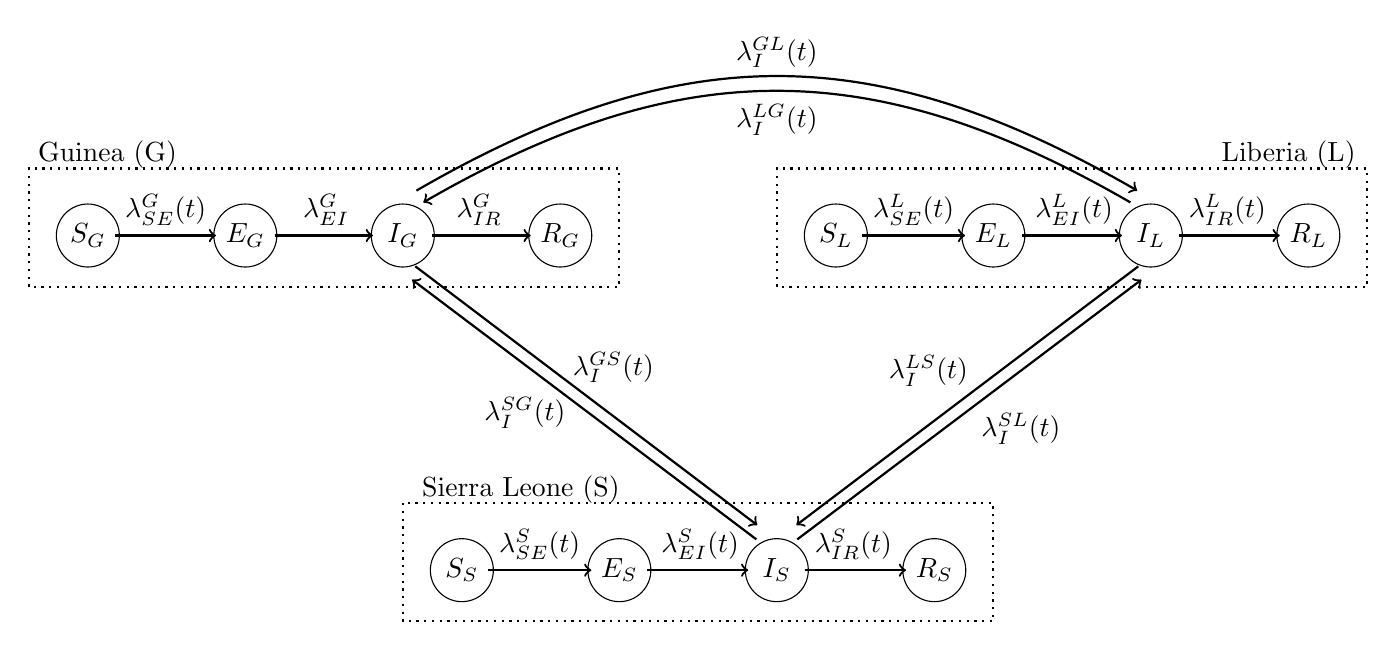
\begin{tikzpicture}
		\draw[thick,dotted] (0,-0.25) rectangle (7.5, 1.25);
		\node at (1, 1) [label=Guinea (G)] {};
		\draw (0.75, 0.4) circle(0.4) node (Sa) {$ S_G $};
		\draw (2.75, 0.4) circle(0.4) node (Ea) {$ E_G $};
		\draw (4.75, 0.4) circle(0.4) node (Ia) {$ I_G $};
		\draw (6.75, 0.4) circle(0.4) node (Ra) {$ R_G $};
		
		\draw[thick,dotted] (9.5,-0.25) rectangle (17, 1.25);
		\node at (16, 1) [label=Liberia (L)] {};	
		\draw (10.25, 0.4) circle(0.4) node (Sb) {$ S_L $};
		\draw (12.25, 0.4) circle(0.4) node (Eb) {$ E_L $};
		\draw (14.25, 0.4) circle(0.4) node (Ib) {$ I_L $};
		\draw (16.25, 0.4) circle(0.4) node (Rb) {$ R_L $};
		
		\draw[thick,dotted] (4.75,-3) rectangle (12.25, -4.5);
		\node at (6.25, -3.25) [label=Sierra Leone (S)] {};	
		\draw (5.5, -3.85) circle(0.4) node (Sc) {$ S_S $};
		\draw (7.5, -3.85) circle(0.4) node (Ec) {$ E_S $};
		\draw (9.5, -3.85) circle(0.4) node (Ic) {$ I_S $};
		\draw (11.5, -3.85) circle(0.4) node (Rc) {$ R_S $};
		
		\draw [thick,->] (Sa) -- (Ea) node[midway,above] {$ \lambda_{SE}^G(t) $};
		\draw [thick,->,shorten >=.6mm] (Ea) -- (Ia) node[midway,above] {$ \lambda_{EI}^G $};
		\draw [thick,->,shorten <=.5mm] (Ia) -- (Ra) node[midway,above] {$ \lambda_{IR}^G $};
		
		\draw [thick,->] (Sb) -- (Eb) node[midway,above] {$ \lambda_{SE}^L(t) $};
		\draw [thick,->,shorten >=.6mm] (Eb) -- (Ib) node[midway,above] {$ \lambda_{EI}^L(t) $};
		\draw [thick,->,shorten <=.5mm] (Ib) -- (Rb) node[midway,above] {$ \lambda_{IR}^L(t) $};
		
		\draw [thick,->] (Sc) -- (Ec) node[midway,above] {$ \lambda_{SE}^S(t) $};
		\draw [thick,->,shorten >=.6mm] (Ec) -- (Ic) node[midway,above] {$ \lambda_{EI}^S(t) $};
		\draw [thick,->,shorten <=.5mm] (Ic) -- (Rc) node[midway,above] {$ \lambda_{IR}^S(t) $};
		
		\path [thick, <-] ([yshift=-0.5mm,xshift=-2mm]Ia.south) edge [shorten >= 2mm, shorten <= 4mm] node [above,xshift=4.5mm,yshift=1.5mm] {$ \lambda_I^{GS}(t) $} ([xshift=-1mm]Ic.north);
		\path [thick, ->] (Ia.south) edge [shorten >= 5mm, shorten <= 2mm] node [below,xshift=-9mm,yshift=2mm] {$ \lambda_I^{SG}(t) $} ([xshift=1.5mm]Ic.north);
		
		\path [thick, <-] ([yshift=-0.5mm,xshift=2mm]Ib.south) edge [shorten >= 2mm, shorten <= 4mm] node[above,yshift=1mm,xshift=-6mm] {$ \lambda_I^{LS}(t) $} ([xshift=1mm]Ic.north);
		\path [thick, ->] (Ib.south) edge [shorten >= 5mm, shorten <= 2mm] node[below,xshift=8mm] {$ \lambda_I^{SL}(t) $} ([xshift=-1.5mm]Ic.north);
		
		\path [thick, <-] ([]Ia.north) edge [shorten >= 3mm, shorten <= 3mm, bend left, looseness=1.1] node [below] {$ \lambda_I^{LG}(t) $} ([]Ib.north);
		\path [thick, ->] ([]Ia.north) edge [shorten >= 2mm, shorten <= 2mm, bend left, looseness=1.1,yshift=2mm] node [above] {$ \lambda_I^{GL}(t) $} ([]Ib.north);		
		\end{tikzpicture}
	}
	\caption[Diagram for a stratified SEIR model with country specific outbreak dynamics and cross--country transmission.]{Diagram of state transitions for a stratified SEIR model used in simulating an outbreak in Guinea, Liberia, and Sierra Leone. Dashed boxes denote countries, nodes in circles denote the model compartments: susceptible (S), exposed (E), infectious (I), recovered (R). Compartments  are subscripted with country indicators. The number of susceptible individuals is equal to the effective population size, estimated as a parameter in the model, minus the numbers of exposed, infected, and recovered individuals. Solid lines with arrows indicate stochastic transitions between model compartments, which occur continuously in time. Rates at which individuals transition between compartments are denoted by $ \lambda $ and are subscripted by compartments and superscripted by countries, e.g., $ \lambda_{SE}^L $ is the rate at which susceptible individuals become exposed in Liberia, $ \lambda_I^{SG} $ is the rate at which an infected individual in Sierra Leone migrates to Guinea. The rate at which susceptible individuals in Guinea become infected is time varying with one changepoint at 33 weeks. Transmission in Liberia and Sierra Leone commenced at 10 and 19 weeks, respectively.Full expressions for the rates are given in Table \ref{tab:ebola_synth_rates_full}.}
	\label{fig:stratified_seir_full_diag}
\end{figure}

\begin{table}[htbp]
	\caption[Week zero, and true and effective population sizes for a simulated Ebola outbreak in West Africa.]{True and effective population sizes, and initial conditions for a simulated outbreak in Guinea, Liberia, and Sierra Leone. Week zero is one week before the first observation is accrued and the time at which within--country transmission was assumed to begin. }
	\label{tab:ebola_synth_consts}
	\footnotesize
	\centering
	\begin{tabular}{lccc}	
		\hline	
		& \textbf{Guinea} & \textbf{Liberia} & \textbf{Sierra Leone} \\\hline
		\textbf{True population size $ (N)$} & 11.8 million & 4.4 million & 7.1 million \\ 
		\textbf{Effective population size $ (N_{eff}) $} & 15,000 & 35,000 & 25,000 \\
		\textbf{Week zero $ (t_0) $} & 0 & 10 & 19 \\
		\textbf{Initial state at $ t_0 $} $ (S_0,E_0,I_0,R_0) $ & (11.8$ \times 10^6$-7, 4, 3, 0) & (4.4$ \times 10^6$-5 3, 2, 0)& (7.1$ \times 10^6$-5, 3, 2, 0) \\
		\hline
		&&&
	\end{tabular} 
\end{table}

\begin{sidewaystable}[htbp]
	\begin{fullpage}
		\caption[Parameters and priors for a simulated Ebola outbreak in West Africa.]{Parameters used to simulate an Ebola outbreak in West Africa using a country--stratified SEIR model, prior distributions, and 95\% prior intervals. Subscripts, $ G,L,S, $ indicate specific countries, or generic countries $ A,B $ if a prior is shared. Effective reproduction numbers are defined with respect to the effective population size as $ R_{eff} = \beta N_{eff} /\mu $.}
		\label{tab:ebola_synth_pars}
		\scriptsize
	\centering
	\begin{tabular}{lcllr}
		\hline
		\textbf{Parameter} & \textbf{Truth} & \textbf{Interpretation} & \textbf{Prior} & \textbf{Median (95\% Interval)} \\ \hline
		$ R_{eff,G}^{(1)}(t),\ t<33 $ & 1.3 & Effective reproduction \#  & $ R_{eff,G}^{(2)} / R_G^{(1)}\sim $ LogNormal(0, 0.5$ ^2 $) & $ R_{eff,G}^{(2)} / R_{eff,G}^{(1)} = $ 1.00 (0.38, 2.66) \\
		$ R_{eff,G}^{(2)}(t),\ t\geq33 $ & 1.2 & Effective reproduction \# & $ R_{eff,G}^{(2)}-1\sim $ LogNormal(log(0.5), 1.1) & $ \implies R_{eff,G}^{(2)} = 1.50 (1.06, 5.32)$ \\
		$ R_{eff,L} $ & 2.0 & Effective reproduction \# & $ R_{eff,L}\sim $ LogNormal(log(0.5), 1.1) & $ \implies R_{eff,L} = 1.50 (1.06, 5.32)$ \\
		$ R_{eff,S} $ & 1.55 & Effective reproduction \# & $ R_{eff,S}\sim $ LogNormal(log(0.5), 1.1) & $ \implies R_{eff,S} = 1.50 (1.06, 5.32)$ \\
		\makecell[l]{$ \alpha_{GS},\alpha_{GL}, \alpha_{LG},$\\
		$ \alpha_{LS},\alpha_{SG}, \alpha_{SL} $} & 0.003 & \makecell[l]{Infectious migration rate \\ from country A to B} & $ 1000\alpha_{AB} \sim$ Exponential(0.25) & \makecell[r]{\# migrations per 1000 infected \\ = 2.78 (0.10, 14.76)}\\ 
		$ \omega_G $ & 1.1 & Rate from $ E_G\rightarrow I_G $ & $ (1/\mu_G)\big/(1/\omega_G) \sim $ LogNormal(0.0, 0.3$ ^2 $) & $ (1/\mu_G)\big/(1/\omega_G) $ = 1.00 (0.56, 1.80) \\
		$ \omega_L $ & 0.85 & Rate from $ E_L\rightarrow I_L $ & $ (1/\mu_L)\big/(1/\omega_L) \sim $ LogNormal(0.0, 0.3$ ^2 $) & $ (1/\mu_L)\big/(1/\omega_L) $ = 1.00 (0.56, 1.80) \\
		$ \omega_S $ & 1 & Rate from $ E_S\rightarrow I_S $ & $ (1/\mu_S)\big/(1/\omega_S) \sim $ LogNormal(0.0, 0.3$ ^2 $) & $ (1/\mu_S)\big/(1/\omega_S) $ = 1.00 (0.56, 1.80) \\
		$ \mu_G $ & $ 1 $ & Rate from $ E_G\rightarrow I_G $ & $ 1/\mu_G\sim $ LogNormal(0, 0.25$ ^2 $) & $ 7/\mu_G = $ 7.0 (4.29, 11.43) \\
		$ \mu_L $ & $ 0.8 $ & Rate from $ E_L\rightarrow I_L $ & $ 1/\mu_L\sim $ LogNormal(0, 0.25$ ^2 $) & $ 7/\mu_L = $ 7.0 (4.29, 11.43) \\
		$ \mu_S $ & $ 1.1 $ & Rate from $ E_S\rightarrow I_S $ & $ 1/\mu_S\sim $ LogNormal(0, 0.25$ ^2 $) & $ 7/\mu_S = $ 7.0 (4.29, 11.43) \\
		$ N_{eff,G} $ & 15,000 & Effective population size & $ N_{eff,G}\sim\mr{Unif}(\sum_{\ell=1}^{L}Y_\ell^G, N_G/4) $& $ N_{eff,G} \in (4032,\ 2.95\times10^6) $ \\
		$ N_{eff,L} $ & 35,000 & Effective population size & $ N_{eff,L}\sim\mr{Unif}(\sum_{\ell=1}^{L}Y_\ell^L, N_L/4) $& $ N_{eff,L} \in (5945,\ 1.1\times10^6) $ \\
		$ N_{eff,S} $ & 25,000 & Effective population size & $ N_{eff,S}\sim\mr{Unif}(\sum_{\ell=1}^{L}Y_\ell^S, N_S/4) $& $ N_{eff,S} \in (9531,\ 1.775\times10^6) $ \\
		$ \rho_G $ & 0.85 & Mean case detection prob. & $ \logit(\rho_G) \sim $ LogNormal(0, 1.4$ ^2 $) & $ \implies \rho_G = 0.5, (0.06, 0.94)$ \\
		$ \rho_L $ & 0.25 & Mean case detection prob. & $ \logit(\rho_L) \sim $ LogNormal(0, 1.4$ ^2 $) & $ \implies \rho_L = 0.5, (0.06, 0.94)$ \\
		$ \rho_S $ & 0.55 & Mean case detection prob. & $ \logit(\rho_S) \sim $ LogNormal(0, 1.4$ ^2 $) & $ \implies \rho_S = 0.5, (0.06, 0.94)$ \\
		$ \phi_G,\ \phi_L, \phi_S $ & 50 & Neg.Binomial overdispersion & $ \log(\phi) \sim $ LogNormal(0, 5$ ^2 $) & $ \implies \rho_G = 1, (5.5\times 10^-5, 1.8\times10^4)$ \\
		\hline
	\end{tabular}
	\end{fullpage}
\end{sidewaystable}

\begin{table}[htbp]
	\caption[Priors for initial compartment volumes for a simulated Ebola outbreak in West Africa]{Priors for the initial compartment volumes at the times when transmission commenced in each country for a simulated Ebola outbreak in West Africa. The initial compartment volumes for each country are assigned independent truncated multivariate normal priors that respect the boundary conditions on the state space of compartment volumes for that country (explained in Section \ref{sec:lna_init_volumes}). If the population size for country A is $ N_A $, and the initial state probability is denoted $ \bp_{0,A} = \bX_{0,A}/N_A  = (S_{0,A}, E_{0,A}, I_{0,A}, R_{0,A})/N_A$, the prior is a truncated multivariate normal approximation of a multinomial distribution with mean $ N_A\bp_{0,A}$ and covariance $ N_A(\bP_{0,A} - \bp_{0,A}\bp_{0,A}^T) $.} 
	\label{tab:ebola_synth_initdist_priors}
	\centering
	\begin{tabular}{lc}
		\hline \textbf{Country} & \textbf{Prior mean initial volumes} ($ \bX_0 $) \\
		\hline
		Guinea & ($ 11.8\times10^6 -7.1$, 4, 3, 0.1) \\
		Liberia & ($ 4.4\times10^6 -5.1$, 3, 2, 0.1) \\
		Sierra Leone & ($ 7.1\times10^6 -5.1$, 3, 2, 0.1) \\
		\hline
	\end{tabular}
\end{table}

\begin{table}[htbp]
	\caption[Transmission rates for the stratified SEIR model with migration of infecteds for Ebola in West Africa.]{Rates of transitions between compartments for the full stratified SEIR model for the spread of Ebola in Guinea, Liberia, and Sierra Leone with cross--country migration of infected individuals across country borders. These rates were used in simulating the outbreak and data, and in the supplementary model presented in Section \ref{subsec:ebola_synth_fullmod_res}. The model is diagrammed in Figure \ref{fig:stratified_seir_full_diag}. Subscripts in the rates denote model compartments, superscripts denote countries. Subscripts for parameters denote countries. The number of susceptible individuals is equal to the effective population size, estimated as a parameter in the model, minus the numbers of exposed, infected, and recovered individuals. The rate at which susceptibles in Guine become infected is time varying with one changepoint at 33 weeks. Transmission in Liberia and Sierra Leone prior to weeks 10 and 19 is expressed in the initial compartment volumes at those times. Thus, all respective transition rates are set to zero prior to the times when transmission commenced in those countries.}
	\label{tab:ebola_synth_rates_full}
	\centering\footnotesize
	\begin{tabular}{llll}
		\hline
		\textbf{From} & \textbf{To} & \textbf{Country} & \textbf{Rate} \\
		\hline
		Susceptible & Exposed & Guinea & $ \lambda_{SE}^G(t) = (\beta_G^{(1)} \ind{t<33} + \beta_G^{(2)}\ind{t\geq33})S_GI_G $ \\
		Susceptible & Exposed & Liberia & $ \lambda_{SE}^L(t) = \beta_LS_LI_L\ind{t\geq10} $\\
		Susceptible & Exposed & Sierra Leone & $ \lambda_{SE}^S(t) = \beta_SS_SI_S\ind{t\geq19} $ \\
		Exposed & Infected & Guinea & $ \lambda_{EI}^G = \omega_GE_G $\\
		Exposed & Infected & Liberia & $ \lambda_{EI}^L(t) = \omega_LE_L\ind{t\geq10} $ \\
		Exposed & Infected & Sierra Leone & $\lambda_{EI}^S(t) = \omega_SE_S\ind{t\geq19}$ \\
		Infected & Recovered & Guinea & $ \lambda_{IR}^G = \mu_GI_G $ \\
		Infected & Recovered & Liberia & $ \lambda_{IR}^L(t) = \mu_LI_L\ind{t\geq10} $ \\	
		Infected & Recovered & Sierra Leone & $ \lambda_{IR}^S(t) = \mu_SI_S\ind{t\geq19} $ \\
		Infected (A) & Infected (B) & Countries A,B & $ \lambda_I ^{AB}(t) = \alpha_{AB}I_A\ind{t\geq{t_{0}^A}}\ind{t\geq t_{0}^B}$\\
		\hline
	\end{tabular}
\end{table}

\begin{table}[htbp]
	\caption[Transmission rates for the stratified SEIR model with virtual migration of infecteds for Ebola in West Africa.]{Approximate rates of transitions between compartments for the stratified SEIR model for the spread of Ebola in Guinea, Liberia, and Sierra Leone with cross--country transmission via virtual migration of infected individuals. These rates were used in the primary model presented in Section \ref{subsec:ebola_synth}. The model is diagrammed in Figure \ref{fig:stratified_seir_full_diag}. Subscripts in the rates denote model compartments, superscripts denote countries. Subscripts for parameters denote countries. The number of susceptible individuals is equal to the effective population size, estimated as a parameter in the model, minus the numbers of exposed, infected, and recovered individuals. The rate at which susceptibles in Guine become infected is time varying with one changepoint at 33 weeks. Transmission in Liberia and Sierra Leone prior to weeks 10 and 19 is expressed in the initial compartment volumes at those times. Thus, all respective transition rates are set to zero prior to the times when transmission commenced in those countries.}
	\label{tab:ebola_synth_rates_approx}
	\centering\footnotesize
	\begin{tabular}{llll}
		\hline
		\textbf{From} & \textbf{To} & \textbf{Country} & \textbf{Rate} \\
		\hline
		Susceptible & Exposed & Guinea & \hspace{-0.7in}\makecell{$ \lambda_{SE}^G(t) = (\beta_G^{(1)} \ind{t<33} + \beta_G^{(2)}\ind{t\geq33})\times $\\
		\hspace{1.25in}$ (I_G + \alpha_{LG}I_L\ind{t\geq10} + \alpha_{SG}I_S\ind{t\geq19})S_G $}\\
		Susceptible & Exposed & Liberia & $ \lambda_{SE}^L(t) = \beta_L(I_L + \alpha_{GL}I_G + \alpha_{SL}I_S\ind{t\geq19})S_L\ind{t\geq10} $\\
		Susceptible & Exposed & Sierra Leone & $ \lambda_{SE}^S(t) = \beta_S(I_S + \alpha_{GS}I_G + \alpha_{LS}I_L)S_S \ind{t\geq19} $ \\
		Exposed & Infected & Guinea & $ \lambda_{EI}^G = \omega_GE_G $\\
		Exposed & Infected & Liberia & $ \lambda_{EI}^L(t) = \omega_LE_L \ind{t\geq10}$ \\
		Exposed & Infected & Sierra Leone & $\lambda_{EI}^S(t) = \omega_SE_S\ind{t\geq19}$ \\
		Infected & Recovered & Guinea & $ \lambda_{IR}^G = \mu_GI_G $ \\
		Infected & Recovered & Liberia & $ \lambda_{IR}^L(t) = \mu_LI_L\ind{t\geq10} $ \\	
		Infected & Recovered & Sierra Leone & $ \lambda_{IR}^S(t) = \mu_SI_S\ind{t\geq19} $ \\
		\hline
	\end{tabular}
\end{table}

\newpage
\subsection{MCMC Details}
\label{subsec:ebola_synth_mcmc}
We fit two models to the simulated data, the true model where migration was modeled explicitly and the approximated model, described in Section \ref{subsec:ebola_synth}, where cross--border transmission was incorporated into the rate of infection via virtual migration. The model fitting procedure and priors were the same for both models. We ran five chains for each model, initialized at random parameter values, for 200,000 iterations per chain. The model parameters, not including the initial compartment volumes, were jointly updated via MVNSS (see Section \ref{subsubsec:mvn_slice_sampling}). The empirical covariance for the MVNSS algorithm was adapted over the first 100,000 iterations using the gain factor sequence, $\gamma_n = 0.5(1 + 0.01n)^{-0.9}$. The contribution of isotropic Gaussian noise to the proposal was initialized at 0.001 and reduced throughout the adaptation phase according to the sequence $ \iota_n = 0.001(1 + 0.01n)^{-0.99} $. The covariance matrix was blocked by country with covariances for parameters belonging to different countries set to zero. Thus, country specific parameters were proposed jointly but were independent in the proposal. Migration parameters were blocked with parameters corresponding to the destination country. The initial compartment volumes were updated jointly with the LNA paths in an EllipSS step. The MCMC alternated between three ElliptSS and two MVNSS updates per MCMC iteration. The ElliptSS bracket width was reset after the first 5,000 MCMC iterations to $ \omega = 2\sqrt{2\log(10)}\sigma_{ElliptSS}$, where $ \sigma_{ElliptSS} $ was the standard deviation of the accepted angles over the initial iterations. The MCMC estimation scales for each country were parameterized as in Table \ref{tab:seir_params_est3} with the one addition being the log ratio of effective reproductive numbers, subtract one, for Guinea, $ \log\left ((R_{eff,G}^{(2)}-1)/(R_{eff,G}^{(1)}-1)\right ) $. Convergence was assessed visually by inspection of traceplots of posterior samples, and via potential scale reduction factors (PSRFs) \cite{brooks1998general} computed via the \texttt{coda} R package \cite{codapackage}. The full model took approximately 9.6 days to run, while the approximate model took about 2.8 days. 

\subsection{Additional Results}
\label{subsec:ebola_synth_supplement}

\begin{table}[htbp]
	\caption[Posterior estimates of initial numbers of exposed, infected, and recovered individuals for a stratified SEIR model fit to simulated Ebola data.]{Posterior estimates of initial numbers of exposed, infected, and recovered individuals for a stratified approximate SEIR model with virtual migration of infecteds fit to simulated Ebola data. The effective number of susceptibles is equal to the effective population size, reported in Table \ref{tab:ebola_synth_ests}, minus the numbers of exposed, infected, and recovered individuals, but is not reported since the effective population size is not marginally identifiable.}
	\label{tab:ebola_synth_initdist_res}
	\centering
	\begin{tabular}{lrl}
		\hline
		\textbf{Parameter} & \textbf{Truth} & \textbf{Estimate} \\ 
		\hline
		$ E_{0,G} $& 4.00 & 4.99 (1.39, 8.66) \\ 
		$ E_{0,G} $& 3.00 & 3.4 (0.6, 6.76) \\ 
		$ E_{0,G} $& 3.00 & 3.16 (0.45, 6.55) \\ 
		$ I_{0,G} $& 3.00 & 3.7 (0.82, 6.91) \\ 
		$ I_{0,L} $& 2.00 & 2.67 (0.45, 5.23) \\ 
		$ I_{0,S} $& 2.00 & 2.46 (0.4, 4.95) \\ 
		$ R_{0,G} $& 0.00 & 0.12 (0.07, 0.16) \\ 
		$ R_{0,L} $	& 0.00 & 0.12 (0.07, 0.17) \\ 
		$ R_{0,S} $& 0.00 & 0.11 (0.06, 0.17) \\ 
		\hline
	\end{tabular}
\end{table}

\begin{table}[htbp]
	\caption[Posterior parameter estimates for full and approximate stratified SEIR models fit to a simulated Ebola outbreak.]{Posterior medians (95\% Bayesian credible intervals) for parameters of the full (Figure \ref{fig:stratified_seir_full_diag}) and approximate (Figure \ref{fig:stratified_seir_approx_diag}) stratified SEIR models fit to a simulated Ebola outbreak. The full model explicitly models cross--border transmission via migration of infected individuals, while the approximate model incorporates cross--border transmission through virtual migrations. Subscripts, $ G,L,S, $ indicate specific countries, or generic countries $ A,B $. Effective reproduction numbers are defined with respect to the effective population size as $ R_{eff} = \beta N_{eff} /\mu $. Parameter interpretations and priors are given in Table \ref{tab:ebola_synth_pars}.}
	\label{tab:ebola_synth_ests}
	\centering\footnotesize
	\begin{tabular}{ccrr}		
		\hline
		& & \multicolumn{2}{c}{\textbf{Posterior median (95\% BCI)}}\\\cline{3-4}
		\textbf{Parameter} & \textbf{Truth} & \textit{Approximate Model} & \textit{Full Model} \\ 
		\hline
		$ R_{eff,G}^{(1)} $& 1.30 & 1.24 (1.12, 1.44) & 1.23 (1.13, 1.43) \\ 
		$ R_{eff,G}^{(2)} $& 1.20 & 1.28 (1.1, 1.63)& 1.27 (1.13, 1.52) \\ 
		$ R_{eff,L} $& 2.00 & 1.69 (1.37, 2.22) & 2.07 (1.56, 3.06)  \\ 
		$ R_{eff,S} $& 1.55 & 1.54 (1.31, 1.97)& 1.52 (1.31, 1.91) \\ 
		$ 7/\omega_G $& 6.36 & 5.55 (2.92, 10.44)& 3.78 (1.89, 8.21)  \\ 
		$ 7/\omega_L $& 8.24 & 6 (2.78, 11.2)&  8.28 (3.87, 15.19) \\ 
		$ 7/\omega_S $& 7.00 & 6.14 (3.26, 11.22)& 5.67 (2.98, 10.58) \\ 
		$ 7/\mu_G $& 7.00 & 6.19 (4.06, 9.65)& 5.83 (3.46, 9.85) \\ 
		$ 7/\mu_L $ & 8.75 & 6.41 (4.05, 9.95) & 8.96 (5.3, 14.7) \\
		$ 7/\mu_S $& 6.36 & 6.46 (4.17, 10.04)& 6.55 (4.25, 9.89) \\ 
		$ 1000\alpha_{GL} $& 3.00 & 3.46 (0.13, 17.22) & 16.22 (6.32, 35.08) \\ 
		$ 1000\alpha_{GS} $& 3.00 & 3.75 (0.14, 18.93)& 20.8 (8.14, 43.62) \\ 
		$ 1000\alpha_{LG} $& 3.00 & 2.19 (0.12, 8.33)&  8.72 (3.29, 19.35) \\ 
		$ 1000\alpha_{LS} $& 3.00 & 3.03 (0.22, 11.3) & 10.15 (3.44, 22.94)  \\ 
		$ 1000\alpha_{SG} $& 3.00 & 2.96 (0.16, 13.67)&  10.05 (3.46, 22.77) \\ 
		$ 1000\alpha_{SL} $& 3.00 & 2.69 (0.12, 11.51)& 5.58 (2.02, 14.79) \\ 
		$ \rho_GN_{eff,G} $& 12750 & 11570 (7750, 19320) &  11590 (7500, 19560) \\ 
		$ \rho_LN_{eff,L} $& 8750 & 10030 (8070, 14180)& 8560 (7220, 11420) \\ 
		$ \rho_SN_{eff,S} $& 15000 & 14860 (11510, 20580)& 15420 (11740, 21230) \\ 
		$ \phi_{G} $& 50.00 & 59.78 (27.36, 211.88) & 42.87 (22.15, 96.72) \\ 
		$ \phi_{L} $& 50.00 & 46.61 (20.82, 105.31)& 46.62 (20.77, 101.46) \\ 
		$ \phi_{S} $& 50.00 & 33.13 (17.76, 60.48) & 31.02 (16.93, 55.48) \\
		\hline
	\end{tabular}
\end{table}

\begin{table}[htbp]
	\caption{Effective sample sizes and potential scale reduction factors for the stratified SEIR model with virtual migration of infecteds fit to a simulated Ebola outbreak.}
	\centering
	\begin{tabular}{lrr}
		\hline
		\textbf{Parameter} & \textbf{ESS} & \textbf{PSRF} \\ 
		\hline
		$ \log\left (R_{eff,G}^{(2)} / R_{eff,G}^{(1)}\right ) $& 461 & 1.01 \\ 
		$ \log\left (R_{eff,G}^{(2)}\right ) $& 367 & 1.01 \\ 
		$ \log\left (R_{eff,L}\right ) $& 505 & 1.06 \\ 
		$ \log\left (R_{eff,S}\right ) $& 759 & 1.02 \\ 
		$ \log\left (\omega_G / \mu_G\right ) $& 1057 & 1.00 \\ 
		$ \log\left (\omega_L / \mu_L\right ) $& 664 & 1.05 \\ 
		$ \log\left (\omega_S / \mu_S\right ) $& 851 & 1.01 \\ 
		$ \log\left (1/\mu_G\right ) $& 719 & 1.01 \\ 
		$ \log\left (1/\mu_L\right ) $& 692 & 1.04 \\ 
		$ \log\left (1/\mu_S\right ) $& 1038 & 1.01 \\ 
		$ \log\left (1000\alpha_{GL}\right ) $& 712 & 1.03 \\ 
		$ \log\left (1000\alpha_{GS}\right ) $& 813 & 1.04 \\ 
		$ \log\left (1000\alpha_{LG}\right ) $& 344 & 1.13 \\ 
		$ \log\left (1000\alpha_{LS}\right ) $& 539 & 1.09 \\ 
		$ \log\left (1000\alpha_{SG}\right ) $& 494 & 1.03 \\ 
		$ \log\left (1000\alpha_{SL}\right ) $& 641 & 1.10 \\ 
		$ \log\left (\rho_GN_{eff,G}\right ) $& 525 & 1.00 \\ 
		$ \log\left (\rho_LN_{eff,L}\right ) $& 603 & 1.08 \\ 
		$ \log\left (\rho_SN_{eff,S}\right ) $& 1020 & 1.01 \\ 
		$ \logit\left (\rho_G\right ) $& 445 & 1.01 \\ 
		$ \logit\left (\rho_L\right ) $& 354 & 1.04 \\ 
		$ \logit\left (\rho_S\right ) $& 540 & 1.03 \\ 
		$ \log(\phi_G) $& 479 & 1.08 \\ 
		$ \log(\phi_L) $& 999 & 1.00 \\ 
		$ \log(\phi_S) $& 1012 & 1.01 \\ 
		\hline
	\end{tabular}
\end{table}

\begin{sidewaysfigure}[htbp]
	\centering
	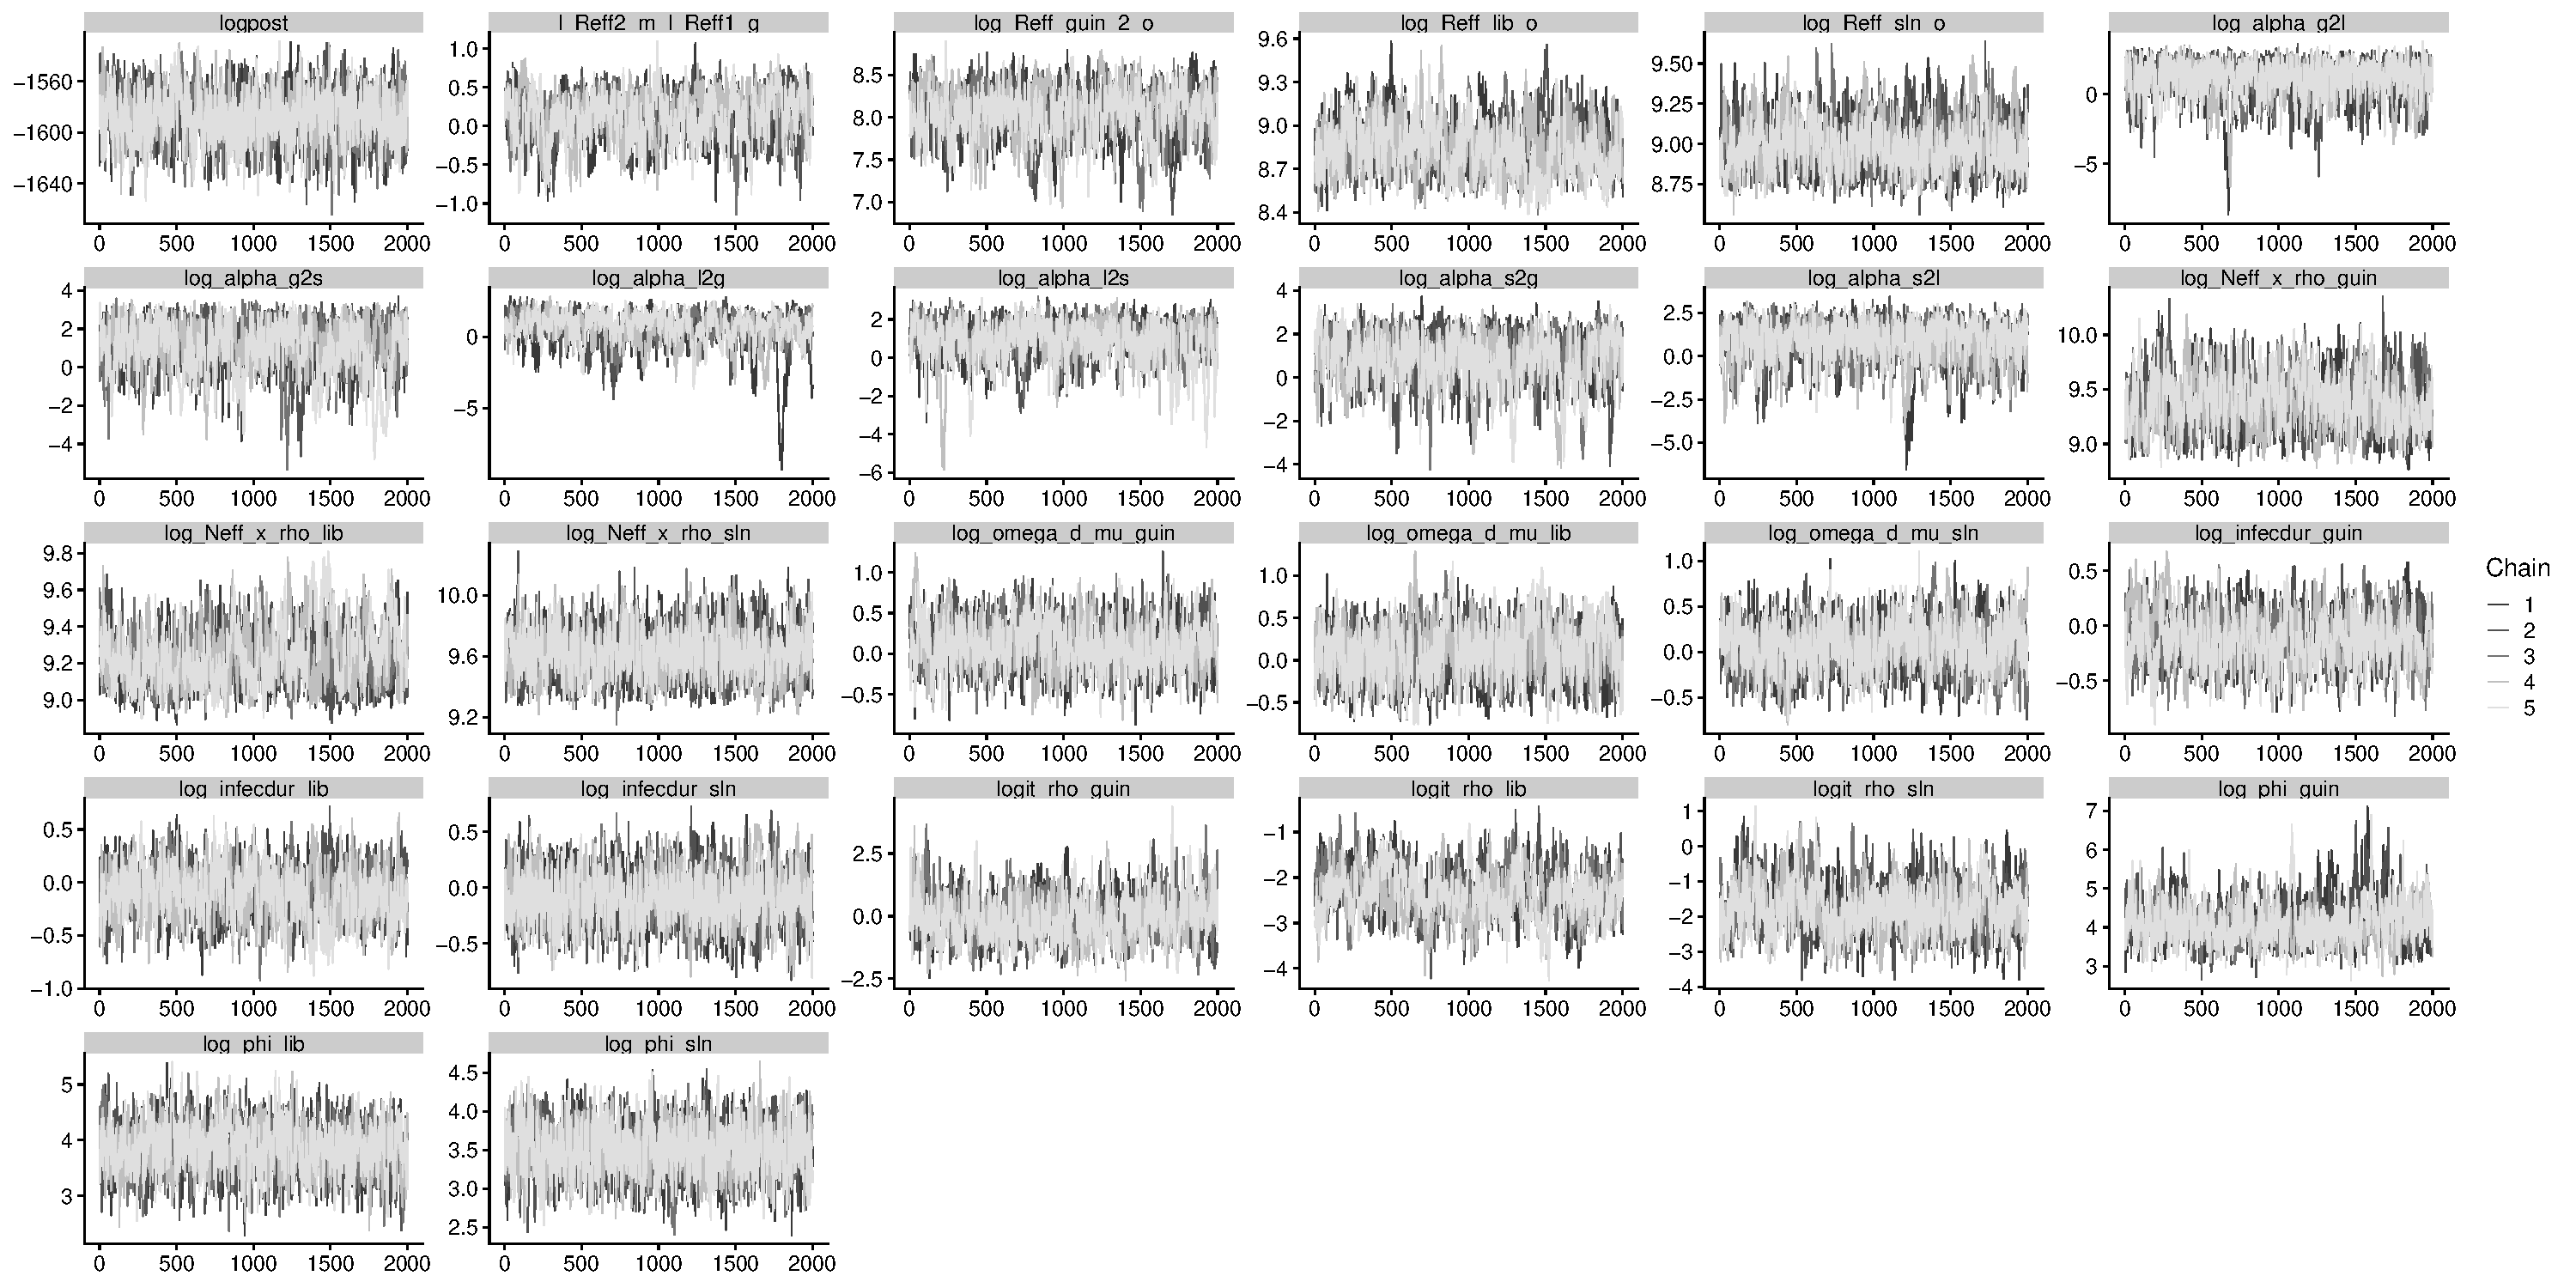
\includegraphics[width=\linewidth]{figures/ebola_synth_traces}
	\caption{Posterior traceplots for a stratified SEIR model fit to a simulated Ebola outbreak.}
	\label{fig:ebolasynthtraces}
\end{sidewaysfigure}

\begin{figure}[htbp]
	\centering
	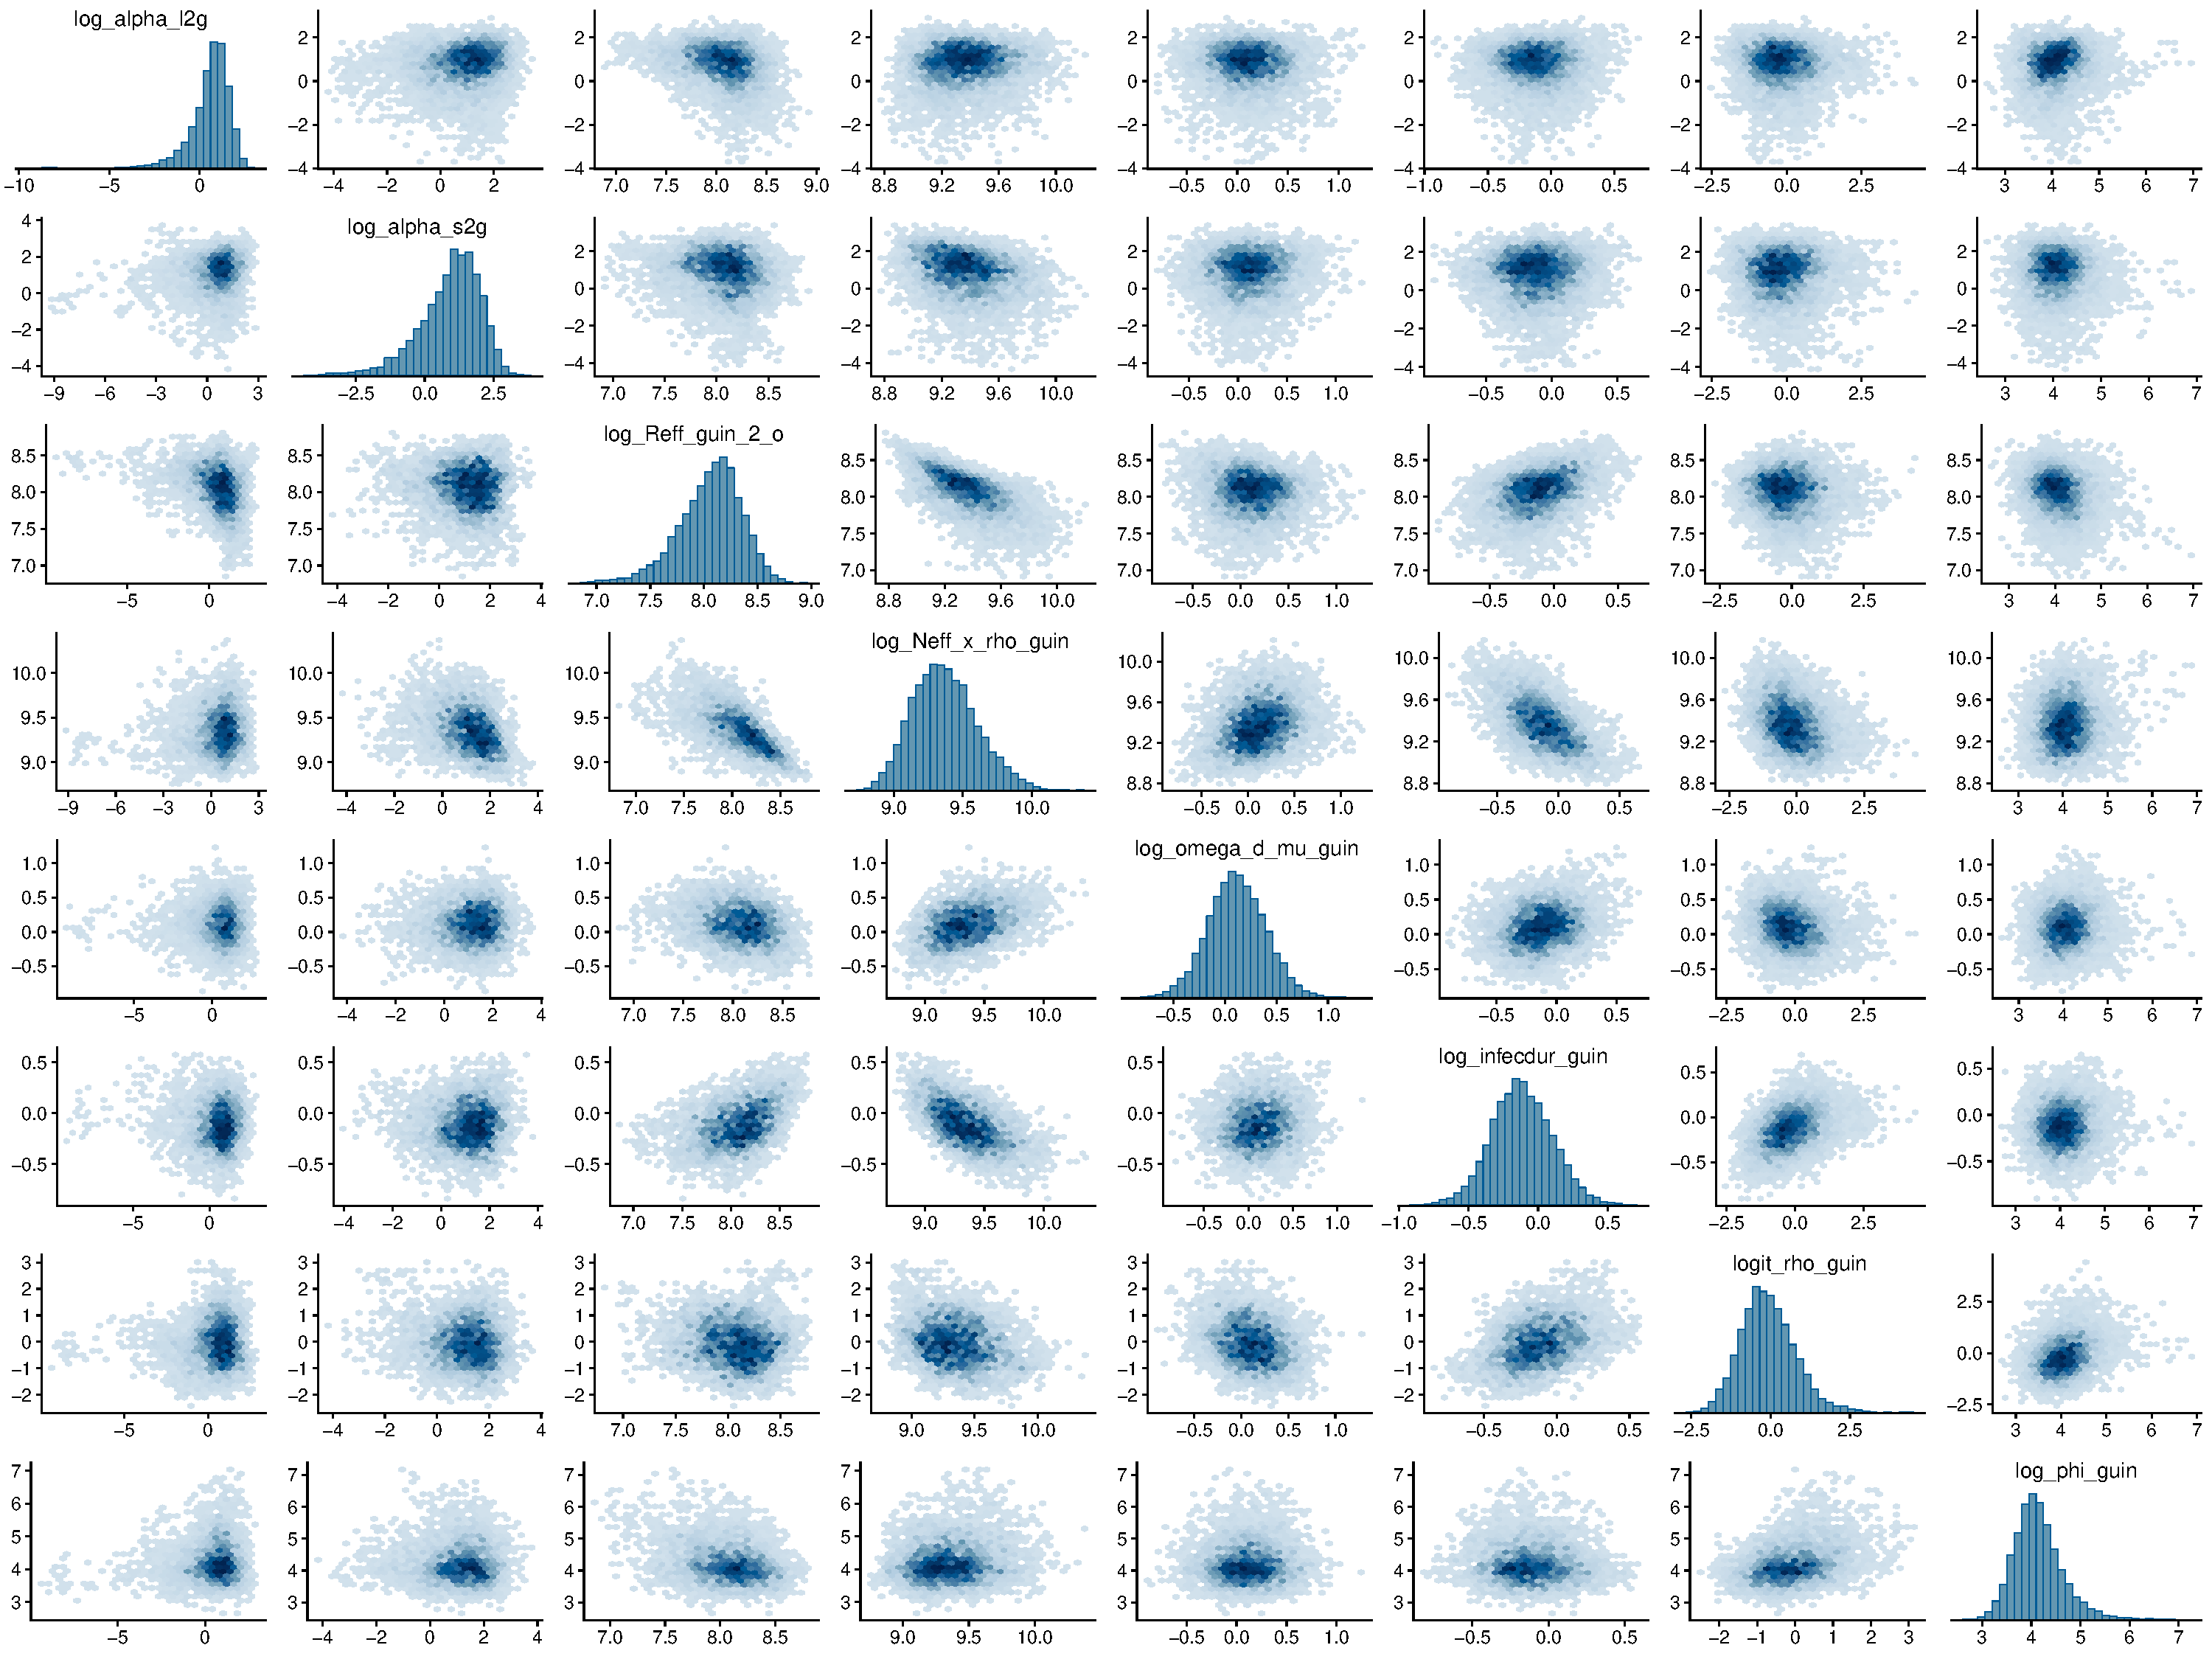
\includegraphics[width=\linewidth]{figures/ebola_synth_pairs_guin}
	\caption{Scatterplots of Guinea--specific parameters in a stratified SEIR model for a simulated Ebola outbreak.}
\end{figure}

\begin{figure}[htbp]
	\centering
	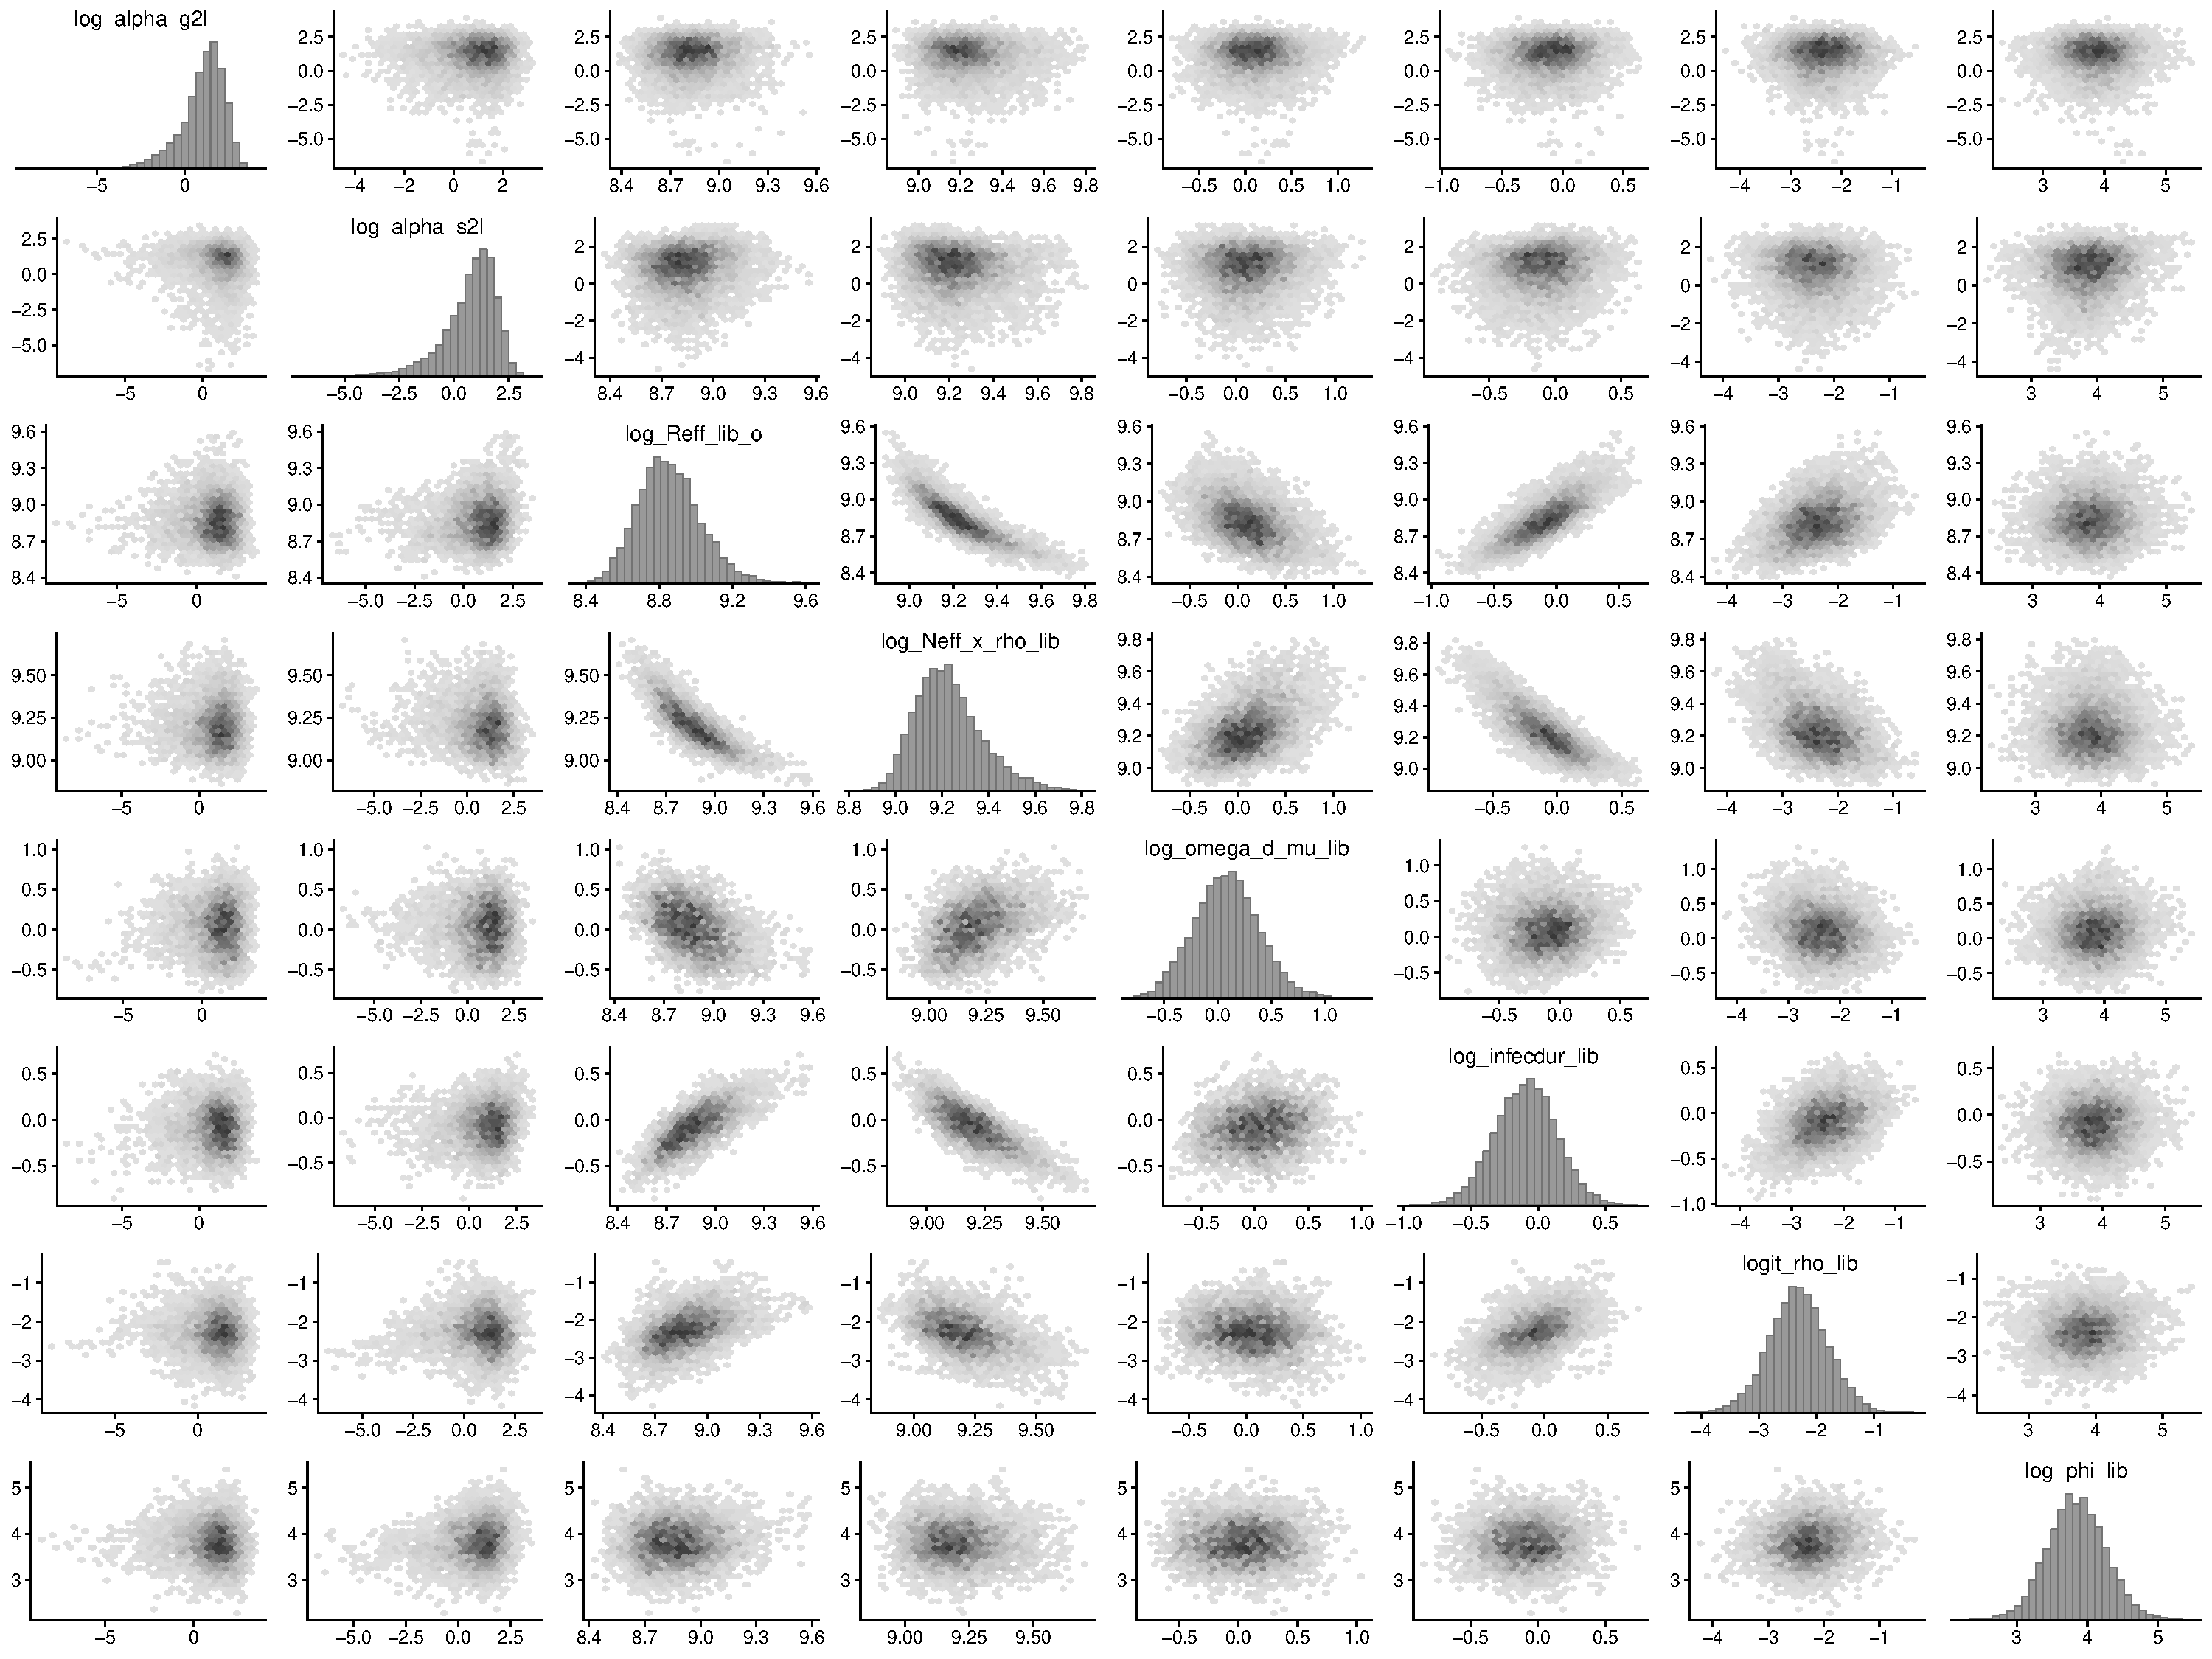
\includegraphics[width=\linewidth]{figures/ebola_synth_pairs_lib}
	\caption{Scatterplots of Liberia--specific parameters in a stratified SEIR model for a simulated Ebola outbreak.}
\end{figure}

\begin{figure}[htbp]
	\centering
	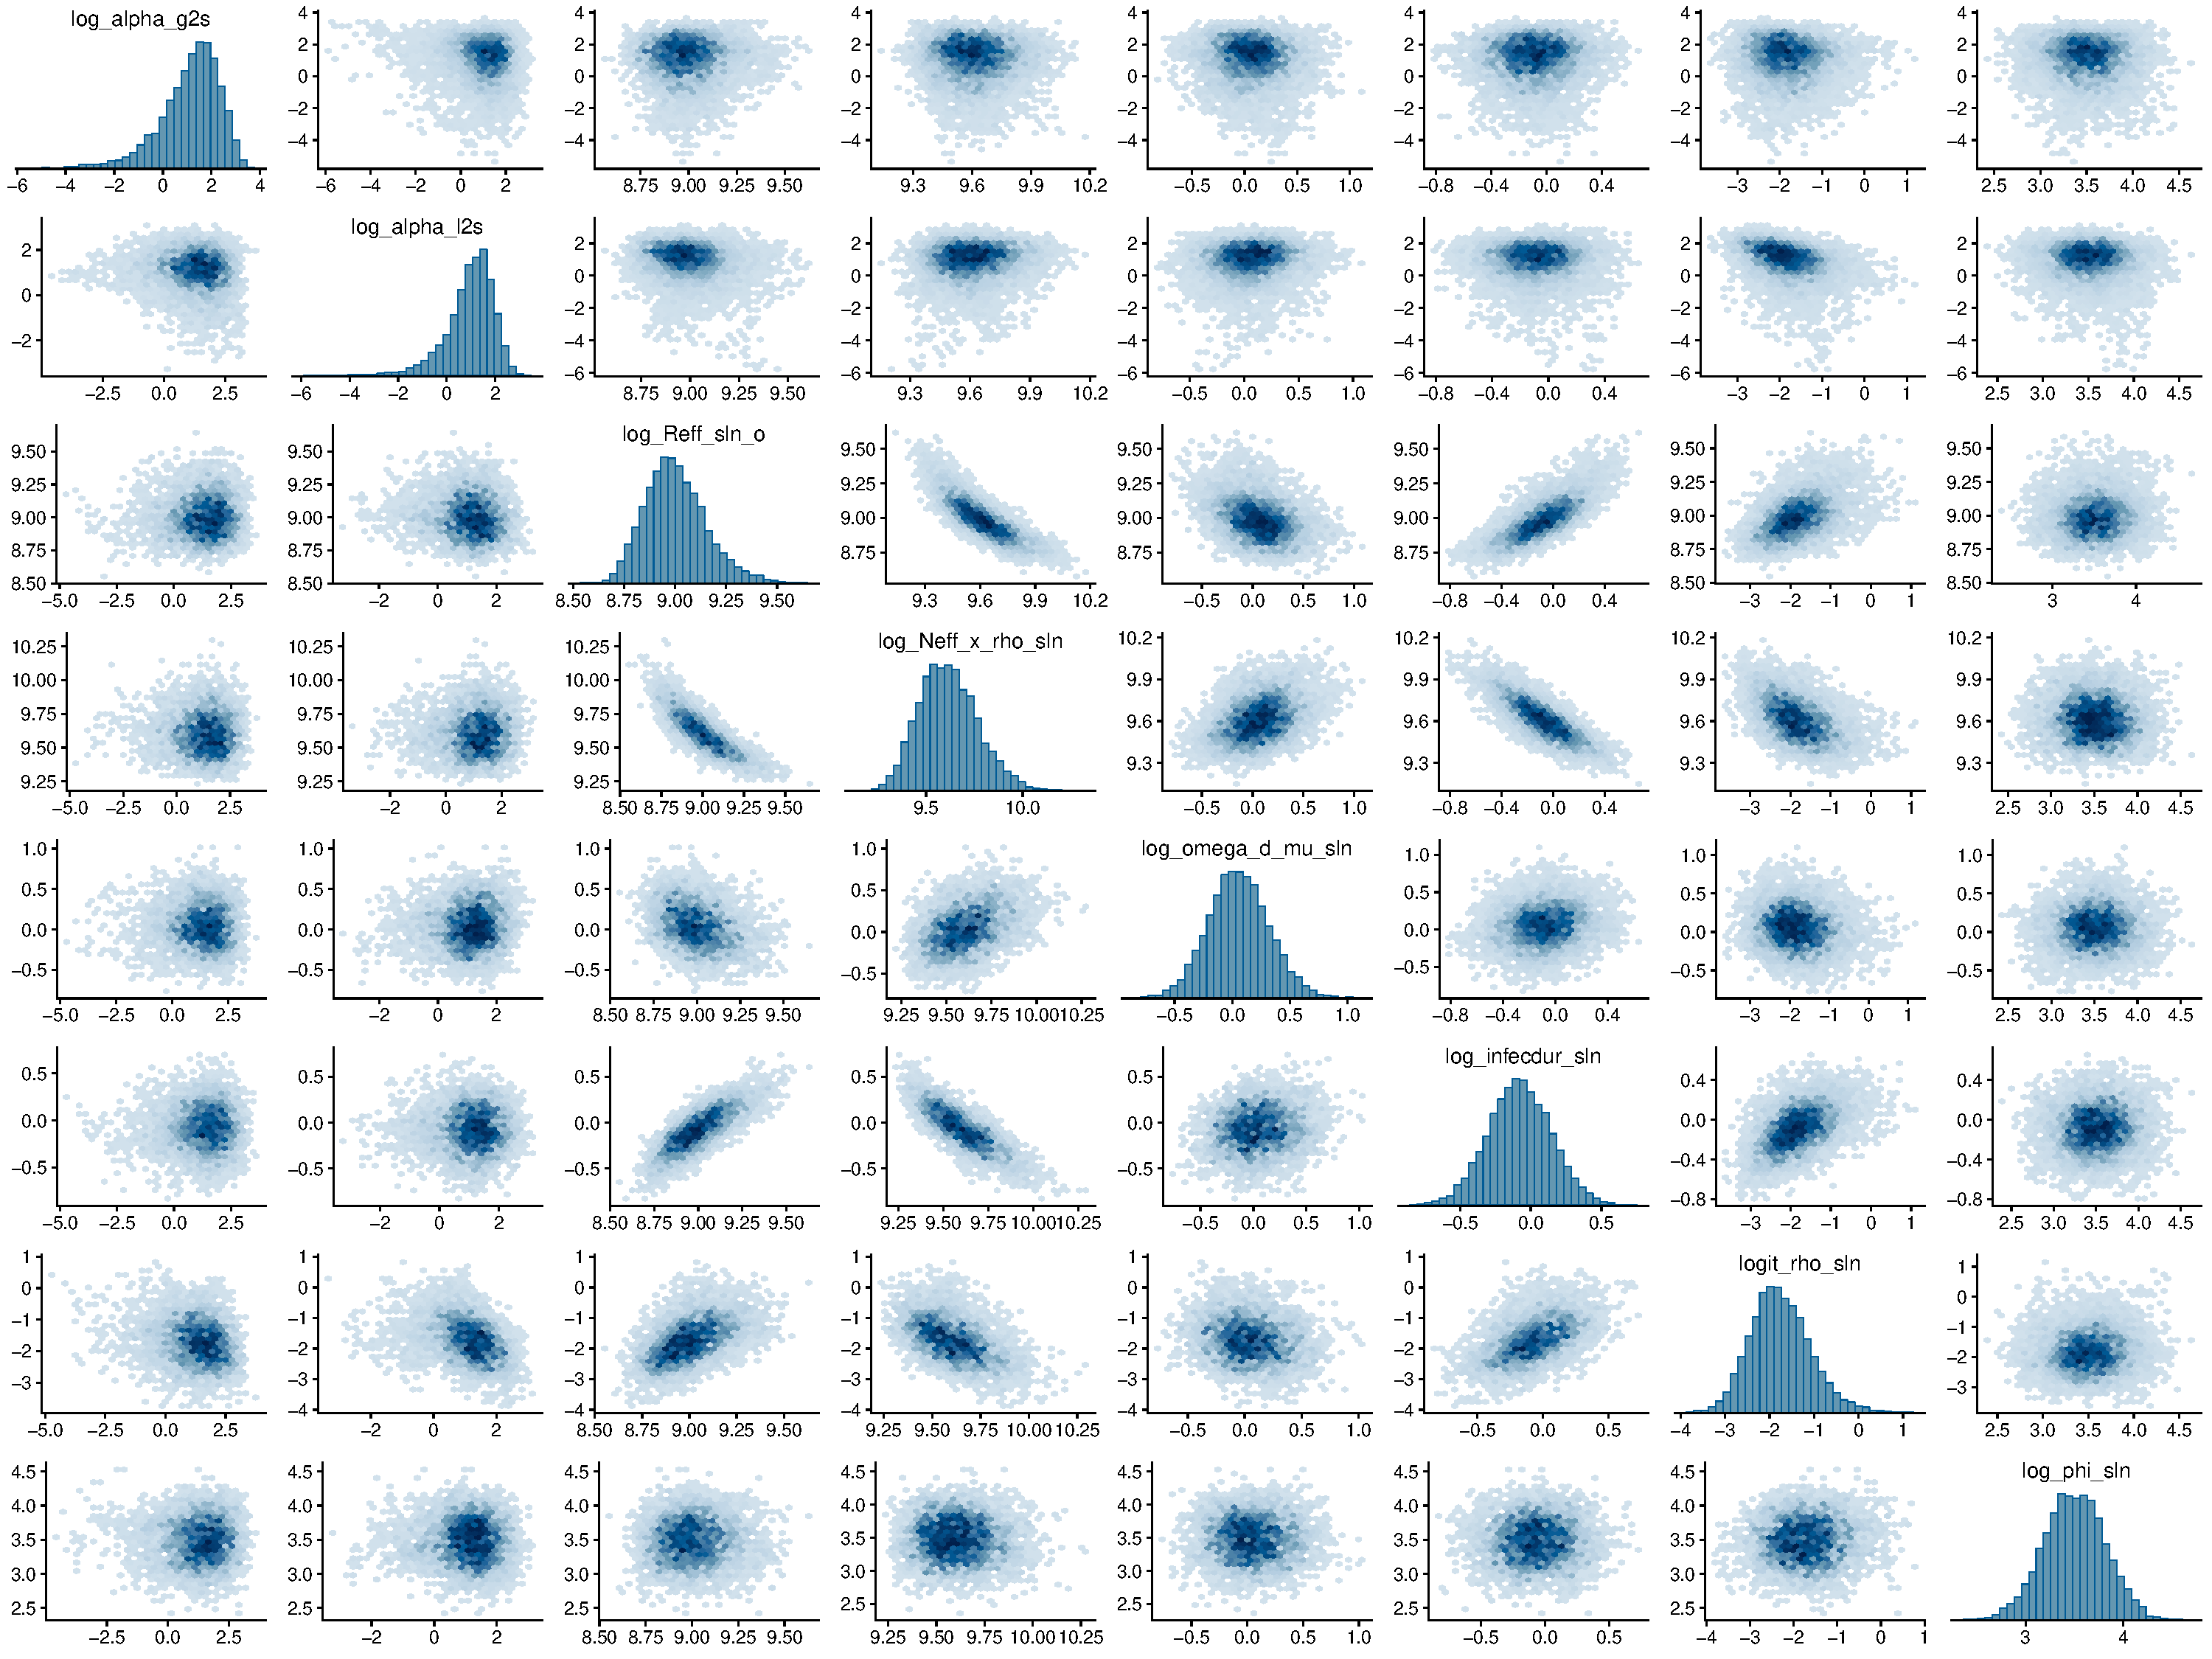
\includegraphics[width=\linewidth]{figures/ebola_synth_pairs_sln}
	\caption{Scatterplots of Sierra Leone--specific parameters in a stratified SEIR model for a simulated Ebola outbreak.}
\end{figure}

\newpage
\section{Modeling Ebola in West Africa --- MCMC Details and Supplementary Results}
\label{sec:ebola_supplement}

\subsection{Details and Supplementary Results for Single--Country Models}
\label{subsec:ebola_single_country_supplement}


\begin{table}[htbp]
	\caption[Transmission rates for single country SEIR models for Ebola in West Africa.]{Rates of transitions between compartments of single country SEIR models, diagrammed in Figure \ref{fig:ebola_single_diag}, for the spread of Ebola in Guinea, Liberia, and Sierra Leone with constant rate of infectious contact from outside the population. Subscripts in the rates denote model compartments, superscripts denote countries. Subscripts for parameters denote countries. The number of susceptible individuals is equal to the effective population size, estimated as a parameter in the model, minus the numbers of exposed, infected, and recovered individuals. The rate at which susceptibles in Guine become infected is time varying with one changepoint at 33 weeks. Transmission in Liberia and Sierra Leone prior to weeks 10 and 19 is expressed in the initial compartment volumes at those times, but is not modeled explicitly.}
	\label{tab:ebola_rates_single}
	\centering\footnotesize
	\begin{tabular}{llll}
		\hline
		\textbf{From} & \textbf{To} & \textbf{Country} & \textbf{Rate} \\
		\hline
		Susceptible & Exposed & Guinea & $ \lambda_{SE}^G(t) = \left (\alpha_G + (\beta_G^{(1)} \ind{t<33} + \beta_G^{(2)}\ind{t\geq33})I_G\right )S_G $ \\
		Susceptible & Exposed & Liberia & $ \lambda_{SE}^L = \left (\alpha_L + \beta_LI_L\right )S_L $\\
		Susceptible & Exposed & Sierra Leone & $ \lambda_{SE}^S = \left (\alpha_S + \beta_SI_S\right )S_S $ \\
		Exposed & Infected & Guinea & $ \lambda_{EI}^G = \omega_GE_G $\\
		Exposed & Infected & Liberia & $ \lambda_{EI}^L(t) = \omega_LE_L $ \\
		Exposed & Infected & Sierra Leone & $\lambda_{EI}^S = \omega_SE_S$ \\
		Infected & Recovered & Guinea & $ \lambda_{IR}^G = \mu_GI_G $ \\
		Infected & Recovered & Liberia & $ \lambda_{IR}^L = \mu_LI_L $ \\	
		Infected & Recovered & Sierra Leone & $ \lambda_{IR}^S = \mu_SI_S$ \\
		\hline
	\end{tabular}
\end{table}

\subsubsection{Priors and MCMC details}
\label{subsubsec:ebola_single_mcmc}

We fit country specific SEIR models to the Ebola incidence data from Guinea, Liberia, and Sierra Leone under two prior regimes given in Tables \ref{tab:ebola_priors_single_tight} and \ref{tab:ebola_priors_single_diff}. The model fitting procedure and priors were the same for all models. We ran five chains for each model, initialized at random parameter values, for 200,000 iterations per chain. The model parameters, not including the initial compartment volumes, were jointly updated via MVNSS (see Section \ref{subsubsec:mvn_slice_sampling}). The empirical covariance for the MVNSS algorithm was adapted over the first 100,000 iterations using the gain factor sequence, $\gamma_n = 0.5(1 + 0.01n)^{-0.9}$. The contribution of isotropic Gaussian noise to the proposal was initialized at 0.001 and reduced throughout the adaptation phase according to the sequence $ \iota_n = 0.001(1 + 0.01n)^{-0.99} $. The initial compartment volumes were updated jointly with the LNA paths in an EllipSS step. The MCMC alternated between two ElliptSS and one MVNSS update per MCMC iteration. The ElliptSS bracket width was reset after the first 5,000 MCMC iterations to $ \omega = 2\sqrt{2\log(10)}\sigma_{ElliptSS}$, where $ \sigma_{ElliptSS} $ was the standard deviation of the accepted angles over the initial iterations. The MCMC estimation scales for each country were parameterized as in Table \ref{tab:seir_params_est3} with the one addition being the log ratio of effective reproductive numbers, subtract one, for Guinea, $ \log\left ((R_{eff,G}^{(2)}-1)/(R_{eff,G}^{(1)}-1)\right ) $. Convergence was assessed visually by inspection of traceplots of posterior samples, and via potential scale reduction factors (PSRFs) \cite{brooks1998general} computed via the \texttt{coda} R package \cite{codapackage}. The models took between 8 hours and 34 hours to run, depending on the speed of the cluster cores. 

\begin{table}[htbp]
	\caption[Priors for initial compartment volumes for single country models fit to data from the Ebola outbreak in West Africa.]{Priors for the initial compartment volumes at the times when transmission commenced in each country for single country models fit to data from the Ebola outbreak in West Africa. The initial compartment volumes for each country are assigned independent truncated multivariate normal priors that respect the boundary conditions on the state space of compartment volumes for that country (explained in Section \ref{sec:lna_init_volumes}). If the population size for country A is $ N_A $, and the initial state probability is denoted $ \bp_{0,A} = \bX_{0,A}/N_A  = (S_{0,A}, E_{0,A}, I_{0,A}, R_{0,A})/N_A$, the prior is a truncated multivariate normal approximation of a multinomial distribution with mean $ N_A\bp_{0,A}$ and covariance $ N_A(\bP_{0,A} - \bp_{0,A}\bp_{0,A}^T) $.} 
	\label{tab:ebola_single_initdist_priors}
	\centering
	\begin{tabular}{lc}
		\hline \textbf{Country} & \textbf{Prior mean initial volumes} ($ \bX_0 $) \\
		\hline
		Guinea & ($ 11.8\times10^6 -7.1$, 4, 3, 0.1) \\
		Liberia & ($ 4.4\times10^6 -5.1$, 3, 2, 0.1) \\
		Sierra Leone & ($ 7.1\times10^6 -5.1$, 3, 2, 0.1) \\
		\hline
	\end{tabular}
\end{table}

\begin{sidewaystable}[htbp]
	\begin{fullpage}
		\caption[Parameters and priors for single country SEIR models fit to the West Africa Ebola outbreak.]{Parameters for a single country SEIR models fit to the West Africa Ebola outbreak, prior distributions used in the main analysis, 95\% prior intervals, and references that informed the choice of priors. Subscripts, $ G,L,S, $ indicate specific countries, or generic countries $ A,B $ if a prior is shared. Effective reproduction numbers are defined with respect to the effective population size as $ R_{eff} = \beta N_{eff} /\mu $.}
		\label{tab:ebola_priors_single_tight}
		\scriptsize
		\centering
		\begin{tabular}{lllrr}
			\hline
			\textbf{Parameter} &  \textbf{Interpretation} & \textbf{Prior} & \textbf{Median (95\% Interval)} & \textbf{References} \\ \hline
			$ R_{eff,G}^{(2)} / R_{eff,G}^{(1)} $ & Ratio of effective reproduction \#s &  LogNormal(0, 0.5$ ^2 $) & $ R_{eff,G}^{(2)} / R_{eff,G}^{(1)} = $ 1.00 (0.38, 2.66) & \cite{chowell2014transmission,chretien2015mathematical,coltart2017ebola,king2015avoidable} \\
			$ R_{eff,G}^{(2)}(t)-1 $ & Effective reproduction \# - 1, $ t\geq33 $ & LogNormal(log(0.5), $ 0.75^2 $) & $ \implies R_{eff,G}^{(2)} = 1.50 (1.11, 3.17)$ &  \cite{chowell2014transmission,chretien2015mathematical,coltart2017ebola,king2015avoidable} \\
			$ R_{eff,L} -1 $ & Effective reproduction \#-1 &  LogNormal(log(0.5), $ 0.75^2 $) & $ \implies R_{eff,L} = 1.50 (1.11, 3.17)$ &  \cite{chowell2014transmission,chretien2015mathematical,coltart2017ebola,king2015avoidable} \\
			$ R_{eff,S}-1 $ & Effective reproduction \#-1 & LogNormal(log(0.5), 0.75$ ^2 $) & $ \implies R_{eff,S} = 1.50 (1.11, 3.17)$ &  \cite{chowell2014transmission,chretien2015mathematical,coltart2017ebola,king2015avoidable}\\
			$ \alpha_{G},\alpha_{L}, \alpha_{S}$ & \makecell[l]{Rate of infectious contact \\ from outside the country} & $ 1000\alpha_{A} \sim$ Exponential(0.25) & \makecell[r]{\# migrations per 1000 infected \\ = 2.78 (0.10, 14.76)} & \cite{dudas2017virus}\\ 
			$ \omega_G/\omega_G $ & Rate from $ E_G\rightarrow I_G $ & LogNormal(0.0, 0.3$ ^2 $) & $ (1/\mu_G)\big/(1/\omega_G) $ = 1.00 (0.56, 1.80) & \cite{chowell2014transmission,velasquez2015time,glynn2017variability} \\
			$ \omega_L/\omega_L $ & Rate from $ E_L\rightarrow I_L $ & LogNormal(0.0, 0.3$ ^2 $) & $ (1/\mu_L)\big/(1/\omega_L) $ = 1.00 (0.56, 1.80) & \cite{chowell2014transmission,velasquez2015time,glynn2017variability} \\
			$ \omega_S/\omega_S $ & Rate from $ E_S\rightarrow I_S $ & LogNormal(0.0, 0.3$ ^2 $) & $ (1/\mu_S)\big/(1/\omega_S) $ = 1.00 (0.56, 1.80) & \cite{chowell2014transmission,velasquez2015time,glynn2017variability} \\
			$ 1/\mu_G $ & Rate from $ E_G\rightarrow I_G $ &  LogNormal(0.3, 0.2$ ^2 $) & $ 7/\mu_G = $ 9.45 (6.38, 13.98) & \cite{chowell2014transmission,velasquez2015time,glynn2017variability} \\
			$ 1/\mu_L $ & Rate from $ E_L\rightarrow I_L $ &  LogNormal(0.3, 0.2$ ^2 $) & $ 7/\mu_L = $ 9.45 (6.38, 13.98) & \cite{chowell2014transmission,velasquez2015time,glynn2017variability} \\
			$ 1/\mu_S $ & Rate from $ E_S\rightarrow I_S $ &  LogNormal(0.3, 0.2$ ^2 $) & $ 7/\mu_S = $ 9.45 (6.38, 13.98) & \cite{chowell2014transmission,velasquez2015time,glynn2017variability} \\
			$ N_{eff,G} $ & Effective population size & $\mr{Unif}(\sum_{\ell=1}^{L}Y_\ell^G, N_G/4) $& $ N_{eff,G} \in (3627,\ 2.95\times10^6) $ & Scale of counts \\
			$ N_{eff,L} $ & Effective population size & $\mr{Unif}(\sum_{\ell=1}^{L}Y_\ell^L, N_L/4) $& $ N_{eff,L} \in (4994,\ 1.1\times10^6) $ & Scale of counts \\
			$ N_{eff,S} $ & Effective population size & $\mr{Unif}(\sum_{\ell=1}^{L}Y_\ell^S, N_S/4) $& $ N_{eff,S} \in (11317,\ 1.775\times10^6) $ & Scale of counts \\
			$ \rho_G $ &  Mean case detection prob. & LogitNormal(0, 1.4$ ^2 $) & $ \implies \rho_G = 0.5, (0.06, 0.94)$ & Very high and very low $ \rho $ unlikely. \\
			$ \rho_L $ &  Mean case detection prob. & LogitNormal(0, 1.4$ ^2 $) & $ \implies \rho_L = 0.5, (0.06, 0.94)$ & Very high and very low $ \rho $ unlikely. \\
			$ \rho_S $ & Mean case detection prob. & LogitNormal(0, 1.4$ ^2 $) & $ \implies \rho_S = 0.5, (0.06, 0.94)$ & Very high and very low $ \rho $ unlikely. \\
			$ \phi_G,\ \phi_L, \phi_S $ &  Neg.Binomial overdispersion & LogNormal(0, 5$ ^2 $) & $ \implies \ = 1, (5.5\times 10^-5, 1.8\times10^4)$ & Diffuse. \\
			\hline
		\end{tabular}
	\end{fullpage}
\end{sidewaystable}

\begin{sidewaystable}[htbp]
	\begin{fullpage}
		\caption[Parameters and priors for supplementary single country SEIR models fit to the West Africa Ebola outbreak.]{Parameters for a single country SEIR models fit to the West Africa Ebola outbreak, prior distributions used in the supplementary analysis, 95\% prior intervals, and references that informed the choice of priors. Subscripts, $ G,L,S, $ indicate specific countries, or generic countries $ A,B $ if a prior is shared. Effective reproduction numbers are defined with respect to the effective population size as $ R_{eff} = \beta N_{eff} /\mu $. Prior distributions for parameters controlling the outbreak dynamics for the supplementary models were more diffuse vis--a--vis the priors in the main analysis.}
		\label{tab:ebola_priors_single_diff}
		\scriptsize
		\centering
		\begin{tabular}{lllrr}
			\hline
			\textbf{Parameter} &  \textbf{Interpretation} & \textbf{Prior} & \textbf{Median (95\% Interval)} & \textbf{References} \\ \hline
			$ R_{eff,G}^{(2)} / R_{eff,G}^{(1)} $ & Ratio of effective reproduction \#s &  LogNormal(0, 0.5$ ^2 $) & $ R_{eff,G}^{(2)} / R_{eff,G}^{(1)} = $ 1.00 (0.38, 2.66) & \cite{chowell2014transmission,chretien2015mathematical,coltart2017ebola,king2015avoidable} \\
			$ R_{eff,G}^{(2)}(t)-1 $ & Effective reproduction \# - 1, $ t\geq33 $ & LogNormal(log(0.5), $ 1.5^2 $) & $ \implies R_{eff,G}^{(2)} = 1.50 (1.02, 10.46)$ &  \cite{chowell2014transmission,chretien2015mathematical,coltart2017ebola,king2015avoidable} \\
			$ R_{eff,L} -1 $ & Effective reproduction \#-1 &  LogNormal(log(0.5), $ 1.5^2 $) & $ \implies R_{eff,L} = 1.50 (1.02, 10.46)$ &  \cite{chowell2014transmission,chretien2015mathematical,coltart2017ebola,king2015avoidable} \\
			$ R_{eff,S}-1 $ & Effective reproduction \#-1 & LogNormal(log(0.5), 1.5$ ^2 $) & $ \implies R_{eff,S} = 1.50 (1.02, 10.46)$ &  \cite{chowell2014transmission,chretien2015mathematical,coltart2017ebola,king2015avoidable}\\
			$ 1000\alpha_{A}$ & \makecell[l]{Rate of infectious contact \\ from outside  country A} & Exponential(0.125) & \makecell[r]{\# migrations per 1000 infected \\ = 5.55 (0.20, 29.51)} & \cite{dudas2017virus}\\ 
			$ \omega_G/\omega_G $ & Rate from $ E_G\rightarrow I_G $ & LogNormal(0.0, 0.3$ ^2 $) & $ (1/\mu_G)\big/(1/\omega_G) $ = 1.00 (0.56, 1.80) & \cite{chowell2014transmission,velasquez2015time,glynn2017variability} \\
			$ \omega_L/\omega_L $ & Rate from $ E_L\rightarrow I_L $ & LogNormal(0.0, 0.3$ ^2 $) & $ (1/\mu_L)\big/(1/\omega_L) $ = 1.00 (0.56, 1.80) & \cite{chowell2014transmission,velasquez2015time,glynn2017variability} \\
			$ \omega_S/\omega_S $ & Rate from $ E_S\rightarrow I_S $ & LogNormal(0.0, 0.3$ ^2 $) & $ (1/\mu_S)\big/(1/\omega_S) $ = 1.00 (0.56, 1.80) & \cite{chowell2014transmission,velasquez2015time,glynn2017variability} \\
			$ 1/\mu_G $ & Rate from $ E_G\rightarrow I_G $ &  LogNormal(0.3, 0.35$ ^2 $) & $ 7/\mu_G = $ 9.45 (4.76, 18.76) & \cite{chowell2014transmission,velasquez2015time,glynn2017variability} \\
			$ 1/\mu_L $ & Rate from $ E_L\rightarrow I_L $ &  LogNormal(0.3, 0.35$ ^2 $) & $ 7/\mu_L = $ 9.45 (4.76, 18.76) & \cite{chowell2014transmission,velasquez2015time,glynn2017variability} \\
			$ 1/\mu_S $ & Rate from $ E_S\rightarrow I_S $ &  LogNormal(0.3, 0.35$ ^2 $) & $ 7/\mu_S = $ 9.45 (4.76, 18.76) & \cite{chowell2014transmission,velasquez2015time,glynn2017variability} \\
			$ N_{eff,G} $ & Effective population size & $\mr{Unif}(\sum_{\ell=1}^{L}Y_\ell^G, N_G/4) $& $ N_{eff,G} \in (3627,\ 2.95\times10^6) $ & Scale of counts \\
			$ N_{eff,L} $ & Effective population size & $\mr{Unif}(\sum_{\ell=1}^{L}Y_\ell^L, N_L/4) $& $ N_{eff,L} \in (4994,\ 1.1\times10^6) $ & Scale of counts \\
			$ N_{eff,S} $ & Effective population size & $\mr{Unif}(\sum_{\ell=1}^{L}Y_\ell^S, N_S/4) $& $ N_{eff,S} \in (11317,\ 1.775\times10^6) $ & Scale of counts \\
			$ \rho_G $ &  Mean case detection prob. & LogitNormal(0, 1.4$ ^2 $) & $ \implies \rho_G = 0.5, (0.06, 0.94)$ & Very high and very low $ \rho $ unlikely. \\
			$ \rho_L $ &  Mean case detection prob. & LogitNormal(0, 1.4$ ^2 $) & $ \implies \rho_L = 0.5, (0.06, 0.94)$ & Very high and very low $ \rho $ unlikely. \\
			$ \rho_S $ & Mean case detection prob. & LogitNormal(0, 1.4$ ^2 $) & $ \implies \rho_S = 0.5, (0.06, 0.94)$ & Very high and very low $ \rho $ unlikely. \\
			$ \phi_G,\ \phi_L, \phi_S $ &  Neg.Binomial overdispersion & LogNormal(0, 5$ ^2 $) & $ \implies \ = 1, (5.5\times 10^-5, 1.8\times10^4)$ & Diffuse. \\
			\hline
		\end{tabular}
	\end{fullpage}
\end{sidewaystable}

\subsubsection{Additional results}
\label{subsubsec:ebola_single_res}


\begin{table}[htbp]
	\caption[Posterior estimates of initial numbers of exposed, infected, and recovered individuals for country--specific SEIR models fit to Ebola outbreak data.]{Posterior estimates of initial numbers of exposed, infected, and recovered individuals for the main country specfic SEIR models fit to Ebola data from the West Africa outbreak under tight priors. The effective number of susceptibles is equal to the effective population size, reported in Table \ref{tab:ebola_single_ests}, minus the numbers of exposed, infected, and recovered individuals, but is not reported since the effective population size is not marginally identifiable.}
	\label{tab:ebola_single_initdist_res}
	\centering
	\begin{tabular}{ll}
		\hline
		\textbf{Parameter} & \textbf{Estimate }\\ 
		\hline
		$ E_{0,G} $& 3.92 (0.7, 7.71) \\ 
		$ I_{0,G} $& 3.01 (0.39, 6.26) \\ 
		$ R_{0,G} $& 0.1 (0.06, 0.15) \\ 
		\hline
		$ E_{0,L} $& 3.12 (0.44, 6.41) \\ 
		$ I_{0,L} $& 2.24 (0.29, 4.81) \\ 
		$ R_{0,L} $& 0.11 (0.06, 0.16) \\ 
		\hline
		$ E_{0,S} $& 1.99 (0.17, 4.73) \\ 
		$ I_{0,S} $& 1.98 (0.22, 4.5) \\ 
		$ R_{0,S} $& 0.09 (0.05, 0.14) \\ 
		\hline
	\end{tabular}
\end{table}

\begin{table}[htbp]
	\caption[Posterior parameter estimates for country--specific SEIR models fit Ebola outbreak data.]{Posterior medians (95\% Bayesian credible intervals) for parameters of the country--specific SEIR models (Figure \ref{fig:ebola_single_diag}) fit to Ebola outbreak data. Subscripts, $ G,L,S, $ indicate specific countries, or generic countries $ A,B $. Effective reproduction numbers are defined with respect to the effective population size as $ R_{eff} = \beta N_{eff} /\mu $. Parameter interpretations and priors are given in Tables \ref{tab:ebola_priors_single_tight} and \ref{tab:ebola_priors_single_diff}. The more informative of the two prior regimes was presented as the main model in Section \ref{subsubsec:ebola_single_models}.}
	\label{tab:ebola_single_ests}
	\centering\footnotesize
	\begin{tabular}{lrr}
		\hline
		& \multicolumn{2}{c}{\textbf{Posterior median (95\% BCI)}}\\\cline{2-3}
		\textbf{Parameter} & \textit{Tight Priors} & \textit{Loose Priors} \\ 
		\hline
		$ R_{eff,G}^{(1)} $& 1.2 (1.1, 1.4) & 1.1 (1.0, 1.4) \\ 
		$ R_{eff,G}^{(2)} $& 1.4 (1.2, 1.8) & 1.2 (1.0, 1.9) \\ 
		$ 7/\omega_G $& 8.4 (4.0, 17.2) & 5.6 (2.2, 18.3) \\ 
		$ 7/\mu_G $& 9.0 (5.9, 13.4) & 6.4 (3.1, 16.0) \\ 
		$ 1000\alpha_{G} $& 0.2 (0.0, 0.6) & 0.1 (0.0, 0.7) \\ 
		$ \rho_GN_{eff,G} $& 7200 (5100, 11900) & 9800 (4900, 34600) \\ 
		$ \phi_{G} $& 4.6 (2.8, 9.4) & 5.8 (3.0, 17.6) \\ 
		\hline
		$ R_{eff,L} $& 2.2 (1.7, 3.3) & 2.7 (1.6, 4.3) \\ 
		$ 7/\omega_L $& 10.5 (4.8, 19.6) & 13.7 (4.6, 23.1) \\ 
		$ 7/\mu_L $& 9.7 (6.6, 14.1) & 11.7 (5.7, 20.3) \\ 
		$ 1000\alpha_L $& 0.0 (0.0, 0.06) & 0.0 (0.0, 0.1) \\ 
		$ \rho_LN_{eff,L} $& 5700 (4600, 7300) & 5300 (4400, 7800) \\ 
		$ \phi_L $& 8.1 (3.7, 17.8) & 8.6 (4.0, 19.2) \\ 
		\hline
		$ R_{eff,S} $& 1.3 (1.2, 1.5) & 1.2 (1.1, 1.4) \\ 
		$ 7/\omega_S $& 4.5 (2.6, 7.4) & 3.5 (1.9, 6.0) \\ 
		$ 7/\mu_S $& 6.2 (4.5, 8.5) & 4.3 (2.6, 6.7) \\ 
		$ 1000\alpha_S $& 0.0 (0, 0.1) & 0.0 (0, 0.1) \\ 
		$ \rho_SN_{eff,S} $& 24300 (19100, 32800) & 30700 (22000, 48700) \\ 
		$ \phi_S $& 46 (22, 112) & 55 (26, 150) \\ 
		\hline
	\end{tabular}
\end{table}

\begin{table}[htbp]
	\caption{Effective sample sizes and potential scale reduction factors for the main stratified SEIR model with virtual migration of infecteds fit to data from the West Africa Ebola outbreak under tight priors.}
	\centering\footnotesize
	\begin{tabular}{lrr}
		\hline
		\textbf{Parameter} & \textbf{ESS} & \textbf{PSRF} \\ 
		\hline
		& 1512 & 1.01 \\ 
		& 2992 & 1.00 \\ 
		& 2573 & 1.00 \\ 
		& 4953 & 1.00 \\ 
		& 3323 & 1.00 \\ 
		& 2564 & 1.00 \\ 
		& 1865 & 1.01 \\ 
		& 1335 & 1.01 \\
		\hline 
		& 1812 & 1.00 \\ 
		& 3595 & 1.00 \\ 
		& 3061 & 1.00 \\ 
		& 4278 & 1.00 \\ 
		& 3495 & 1.00 \\ 
		& 1534 & 1.00 \\ 
		& 4333 & 1.00 \\ 
		\hline
		& 1503 & 1.00 \\ 
		& 949 & 1.01 \\ 
		& 2268 & 1.00 \\ 
		& 1432 & 1.00 \\ 
		& 958 & 1.01 \\ 
		& 2124 & 1.00 \\ 
		& 969 & 1.00 \\ 
		\hline
	\end{tabular}
\end{table}

\begin{sidewaysfigure}[htbp]
	\begin{fullpage}
		\centering
		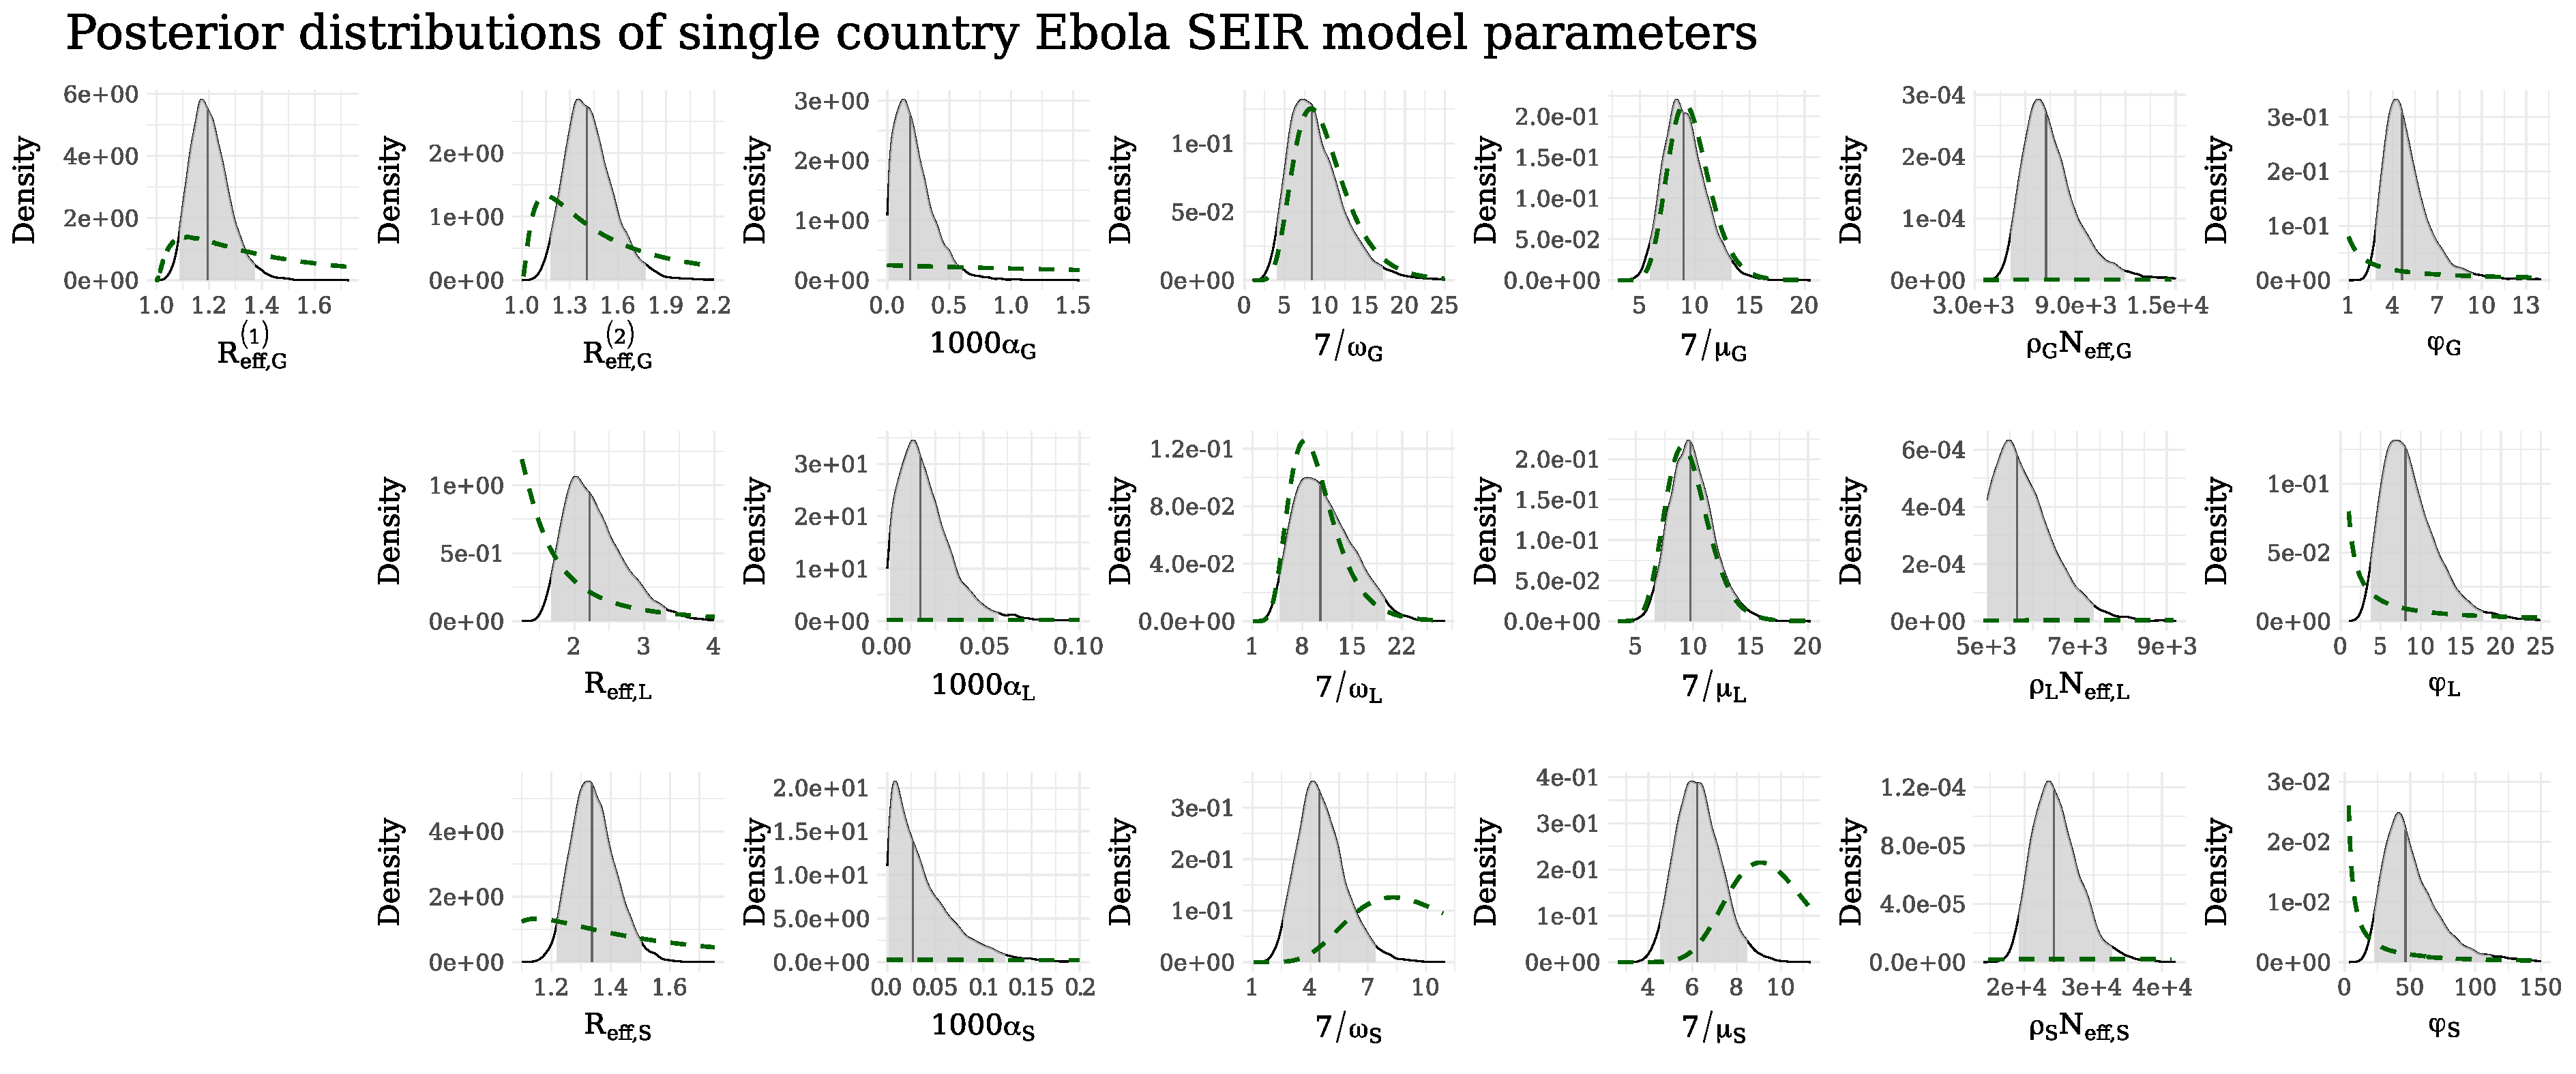
\includegraphics[width=\linewidth]{figures/ebola_single_posts}
		\caption[Posterior distributions of parameters of the main country--specific SEIR models fit to data from the West Africa Ebola outbreak.]{Posterior distributions of parameters for the main country--specific SEIR models fit to data from the West Africa Ebola outbreak. We show posterior medians (solid gray lines), 95\% Bayesian credible intervals (light gray areas under the posterior densities), prior densities (induced priors for the reporting rate and latent period durations) over the posterior ranges (dashed green curves). $ R_{eff} = \beta N_{eff}/\mu $ is the effective reproductive number, where $ \beta $ is the per--contact infection rate, $ N_{eff} $ is the effective population size, and $ \mu $ is the recovery rate. The latent and infectious period durations, $ 7/\omega $ and $ 7/\mu $, respectively, are given in days. The scaled effective number of baseline infectious contacts in country $ A $ is $ 1000\alpha_{A} $. The effective reporting rate is $ \rho N_{eff} $, and $ \phi $ is the negative binomial over--dispersion parameter. Subscripts indicate countries.}
		\label{fig:ebola_single_posts}
	\end{fullpage}
\end{sidewaysfigure}

\begin{sidewaysfigure}[htbp]
	\centering
	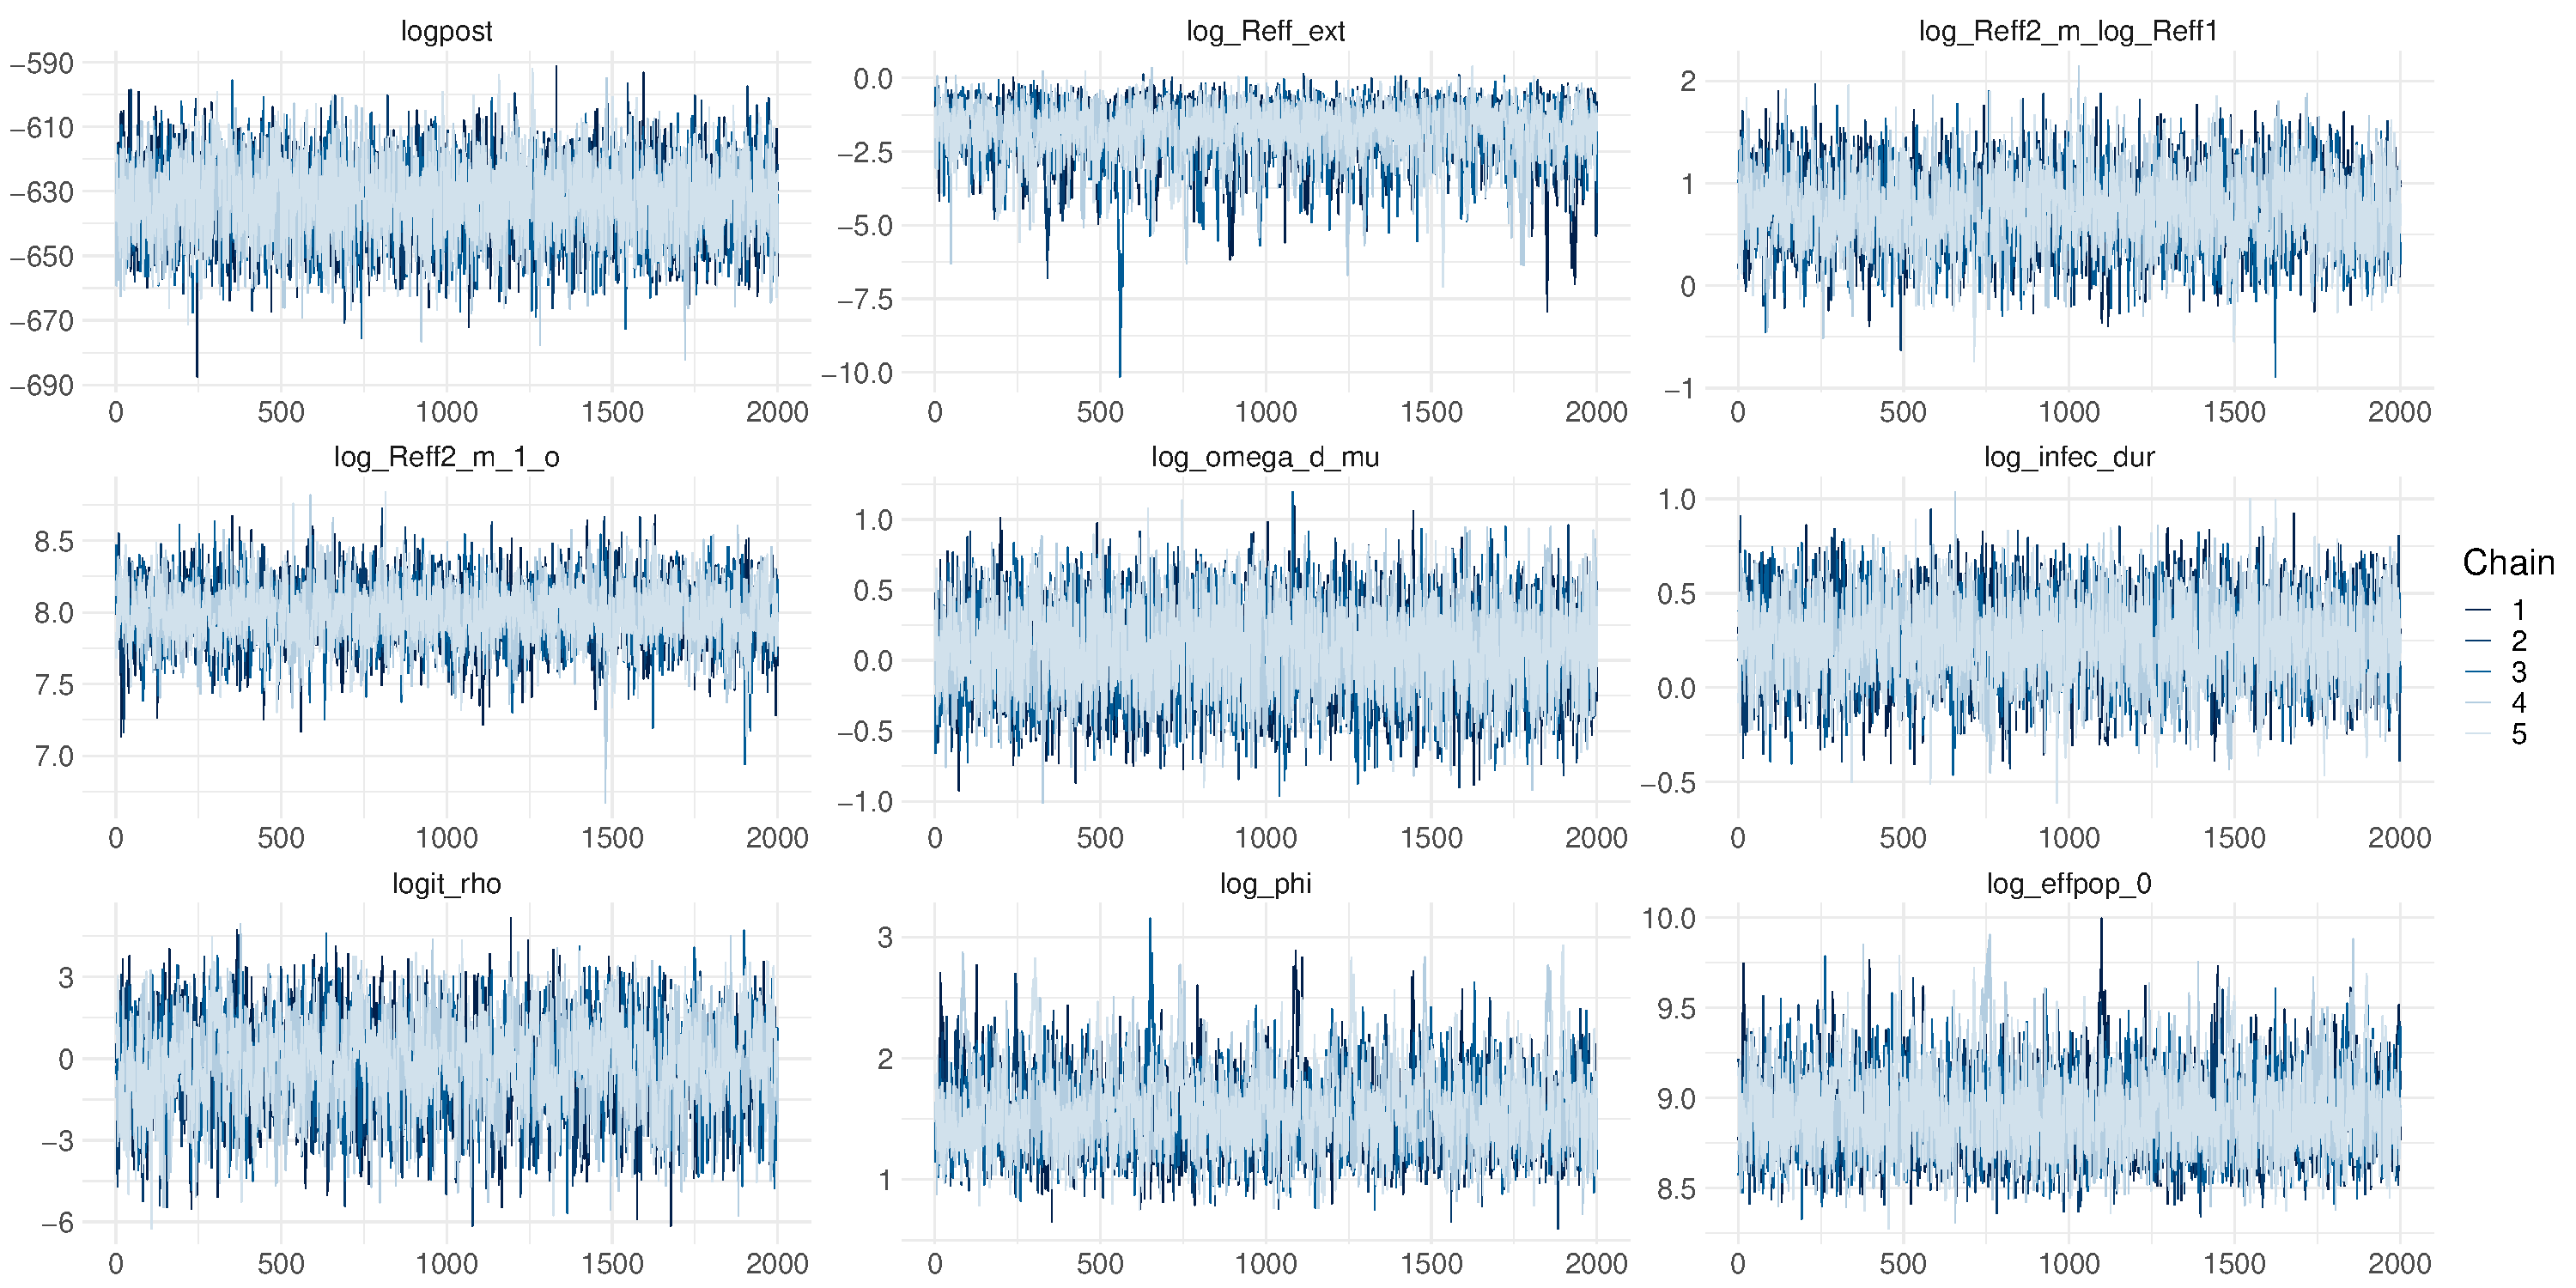
\includegraphics[width=\linewidth]{figures/guin_tight_traces}
	\caption{Posterior traceplots for the SEIR model fit to data from the Ebola outbreak in Guinea.}
	\label{fig:guineatraces}
\end{sidewaysfigure}

\begin{figure}[htbp]
	\centering
	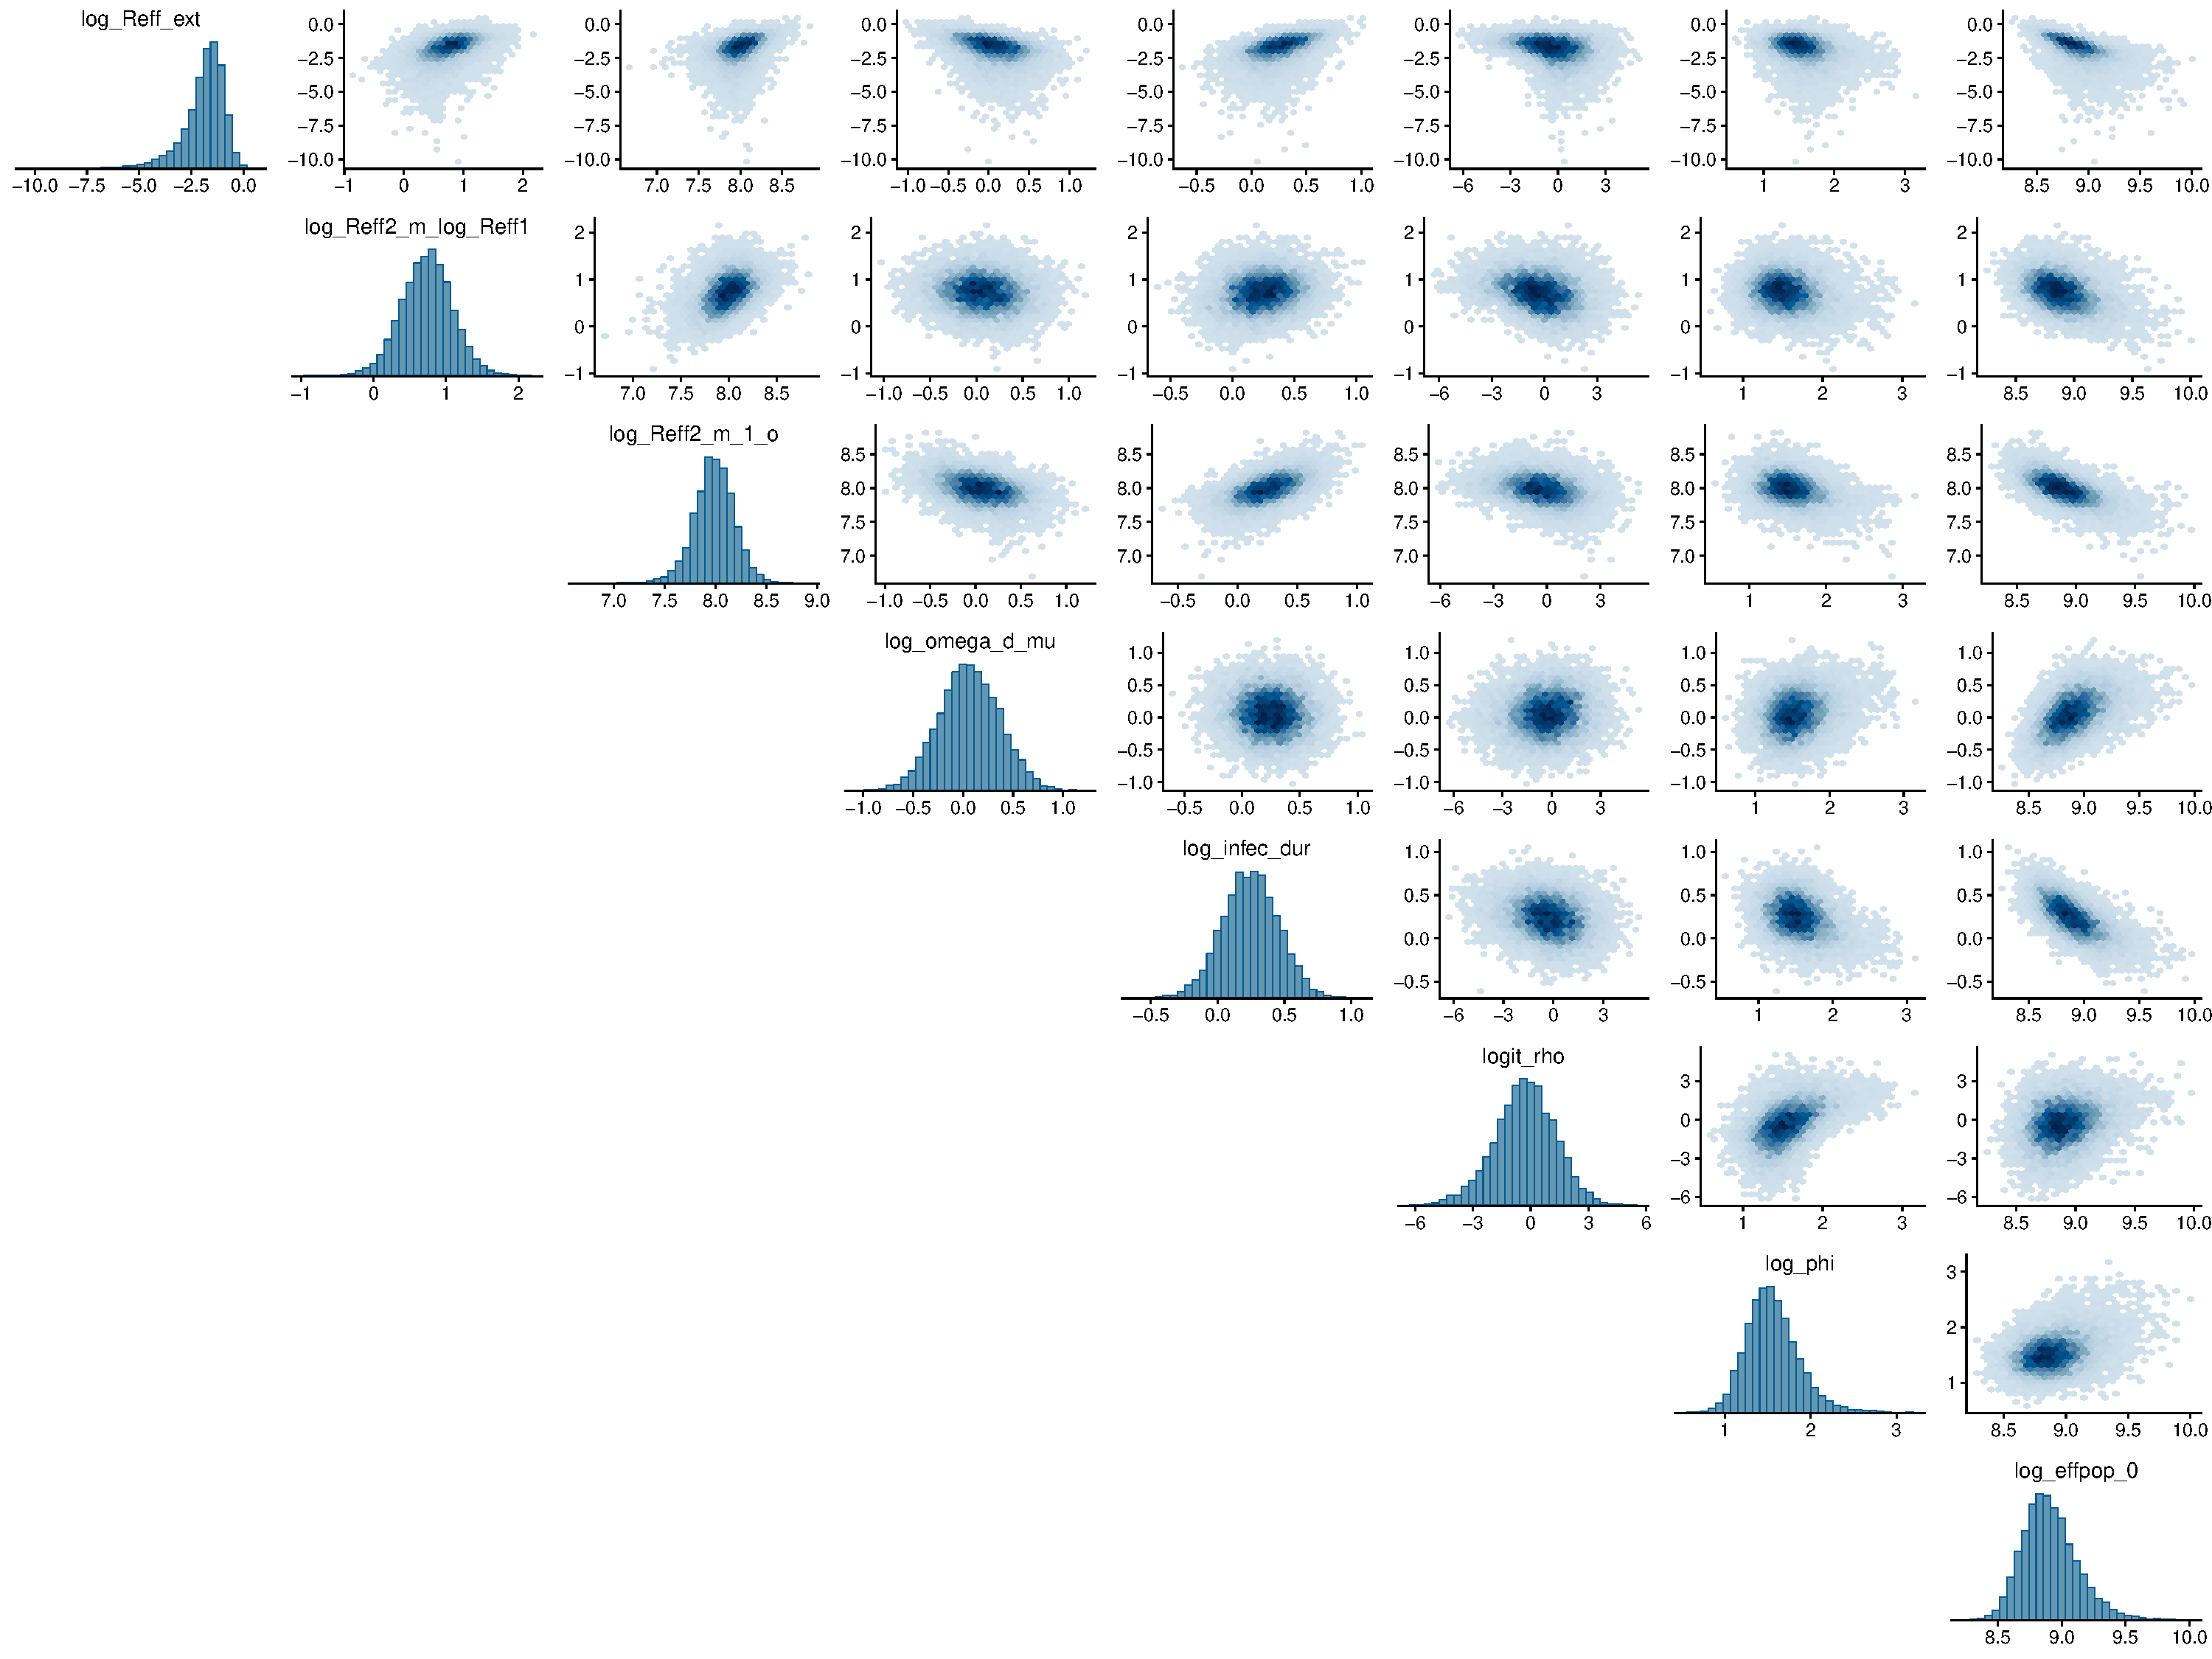
\includegraphics[width=\linewidth]{figures/guin_tight_pairs}
	\caption{Scatterplots of parameters for the SEIR model fit to data from the Ebola outbreak in Guinea.}
	\label{fig:guineapairs}
\end{figure}

\begin{sidewaysfigure}[htbp]
	\centering
	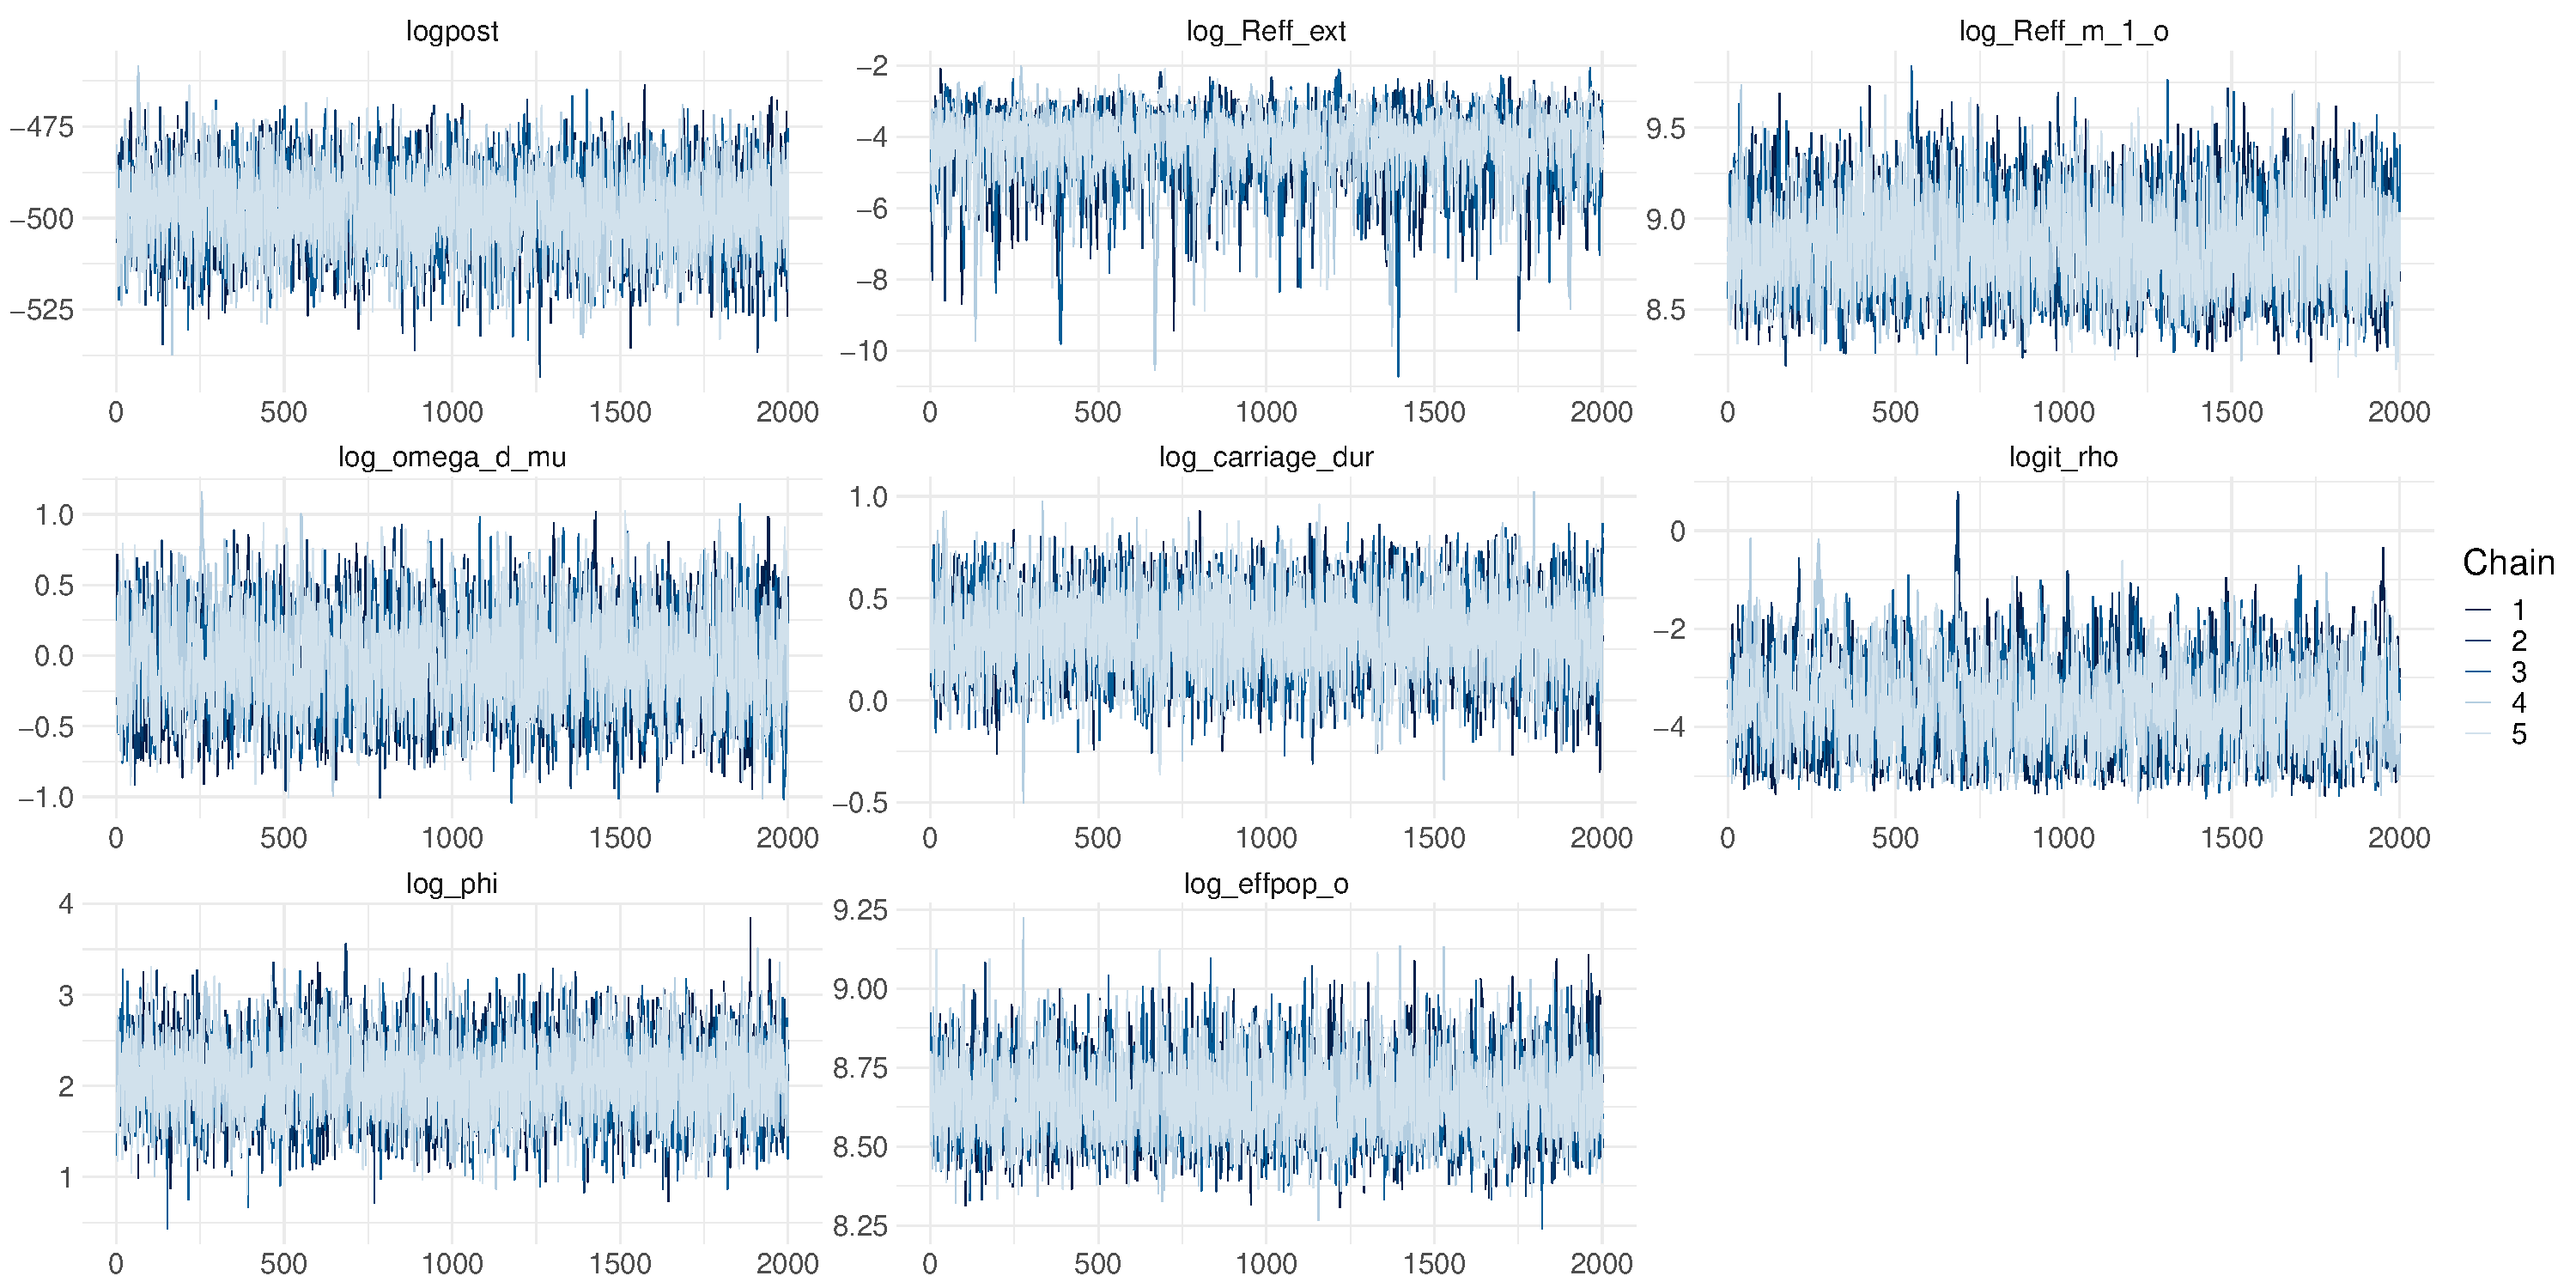
\includegraphics[width=\linewidth]{figures/lib_tight_traces}
	\caption{Posterior traceplots for the SEIR model fit to data from the Ebola outbreak in Liberia.}
	\label{fig:liberiatraces}
\end{sidewaysfigure}

\begin{figure}[htbp]
	\centering
	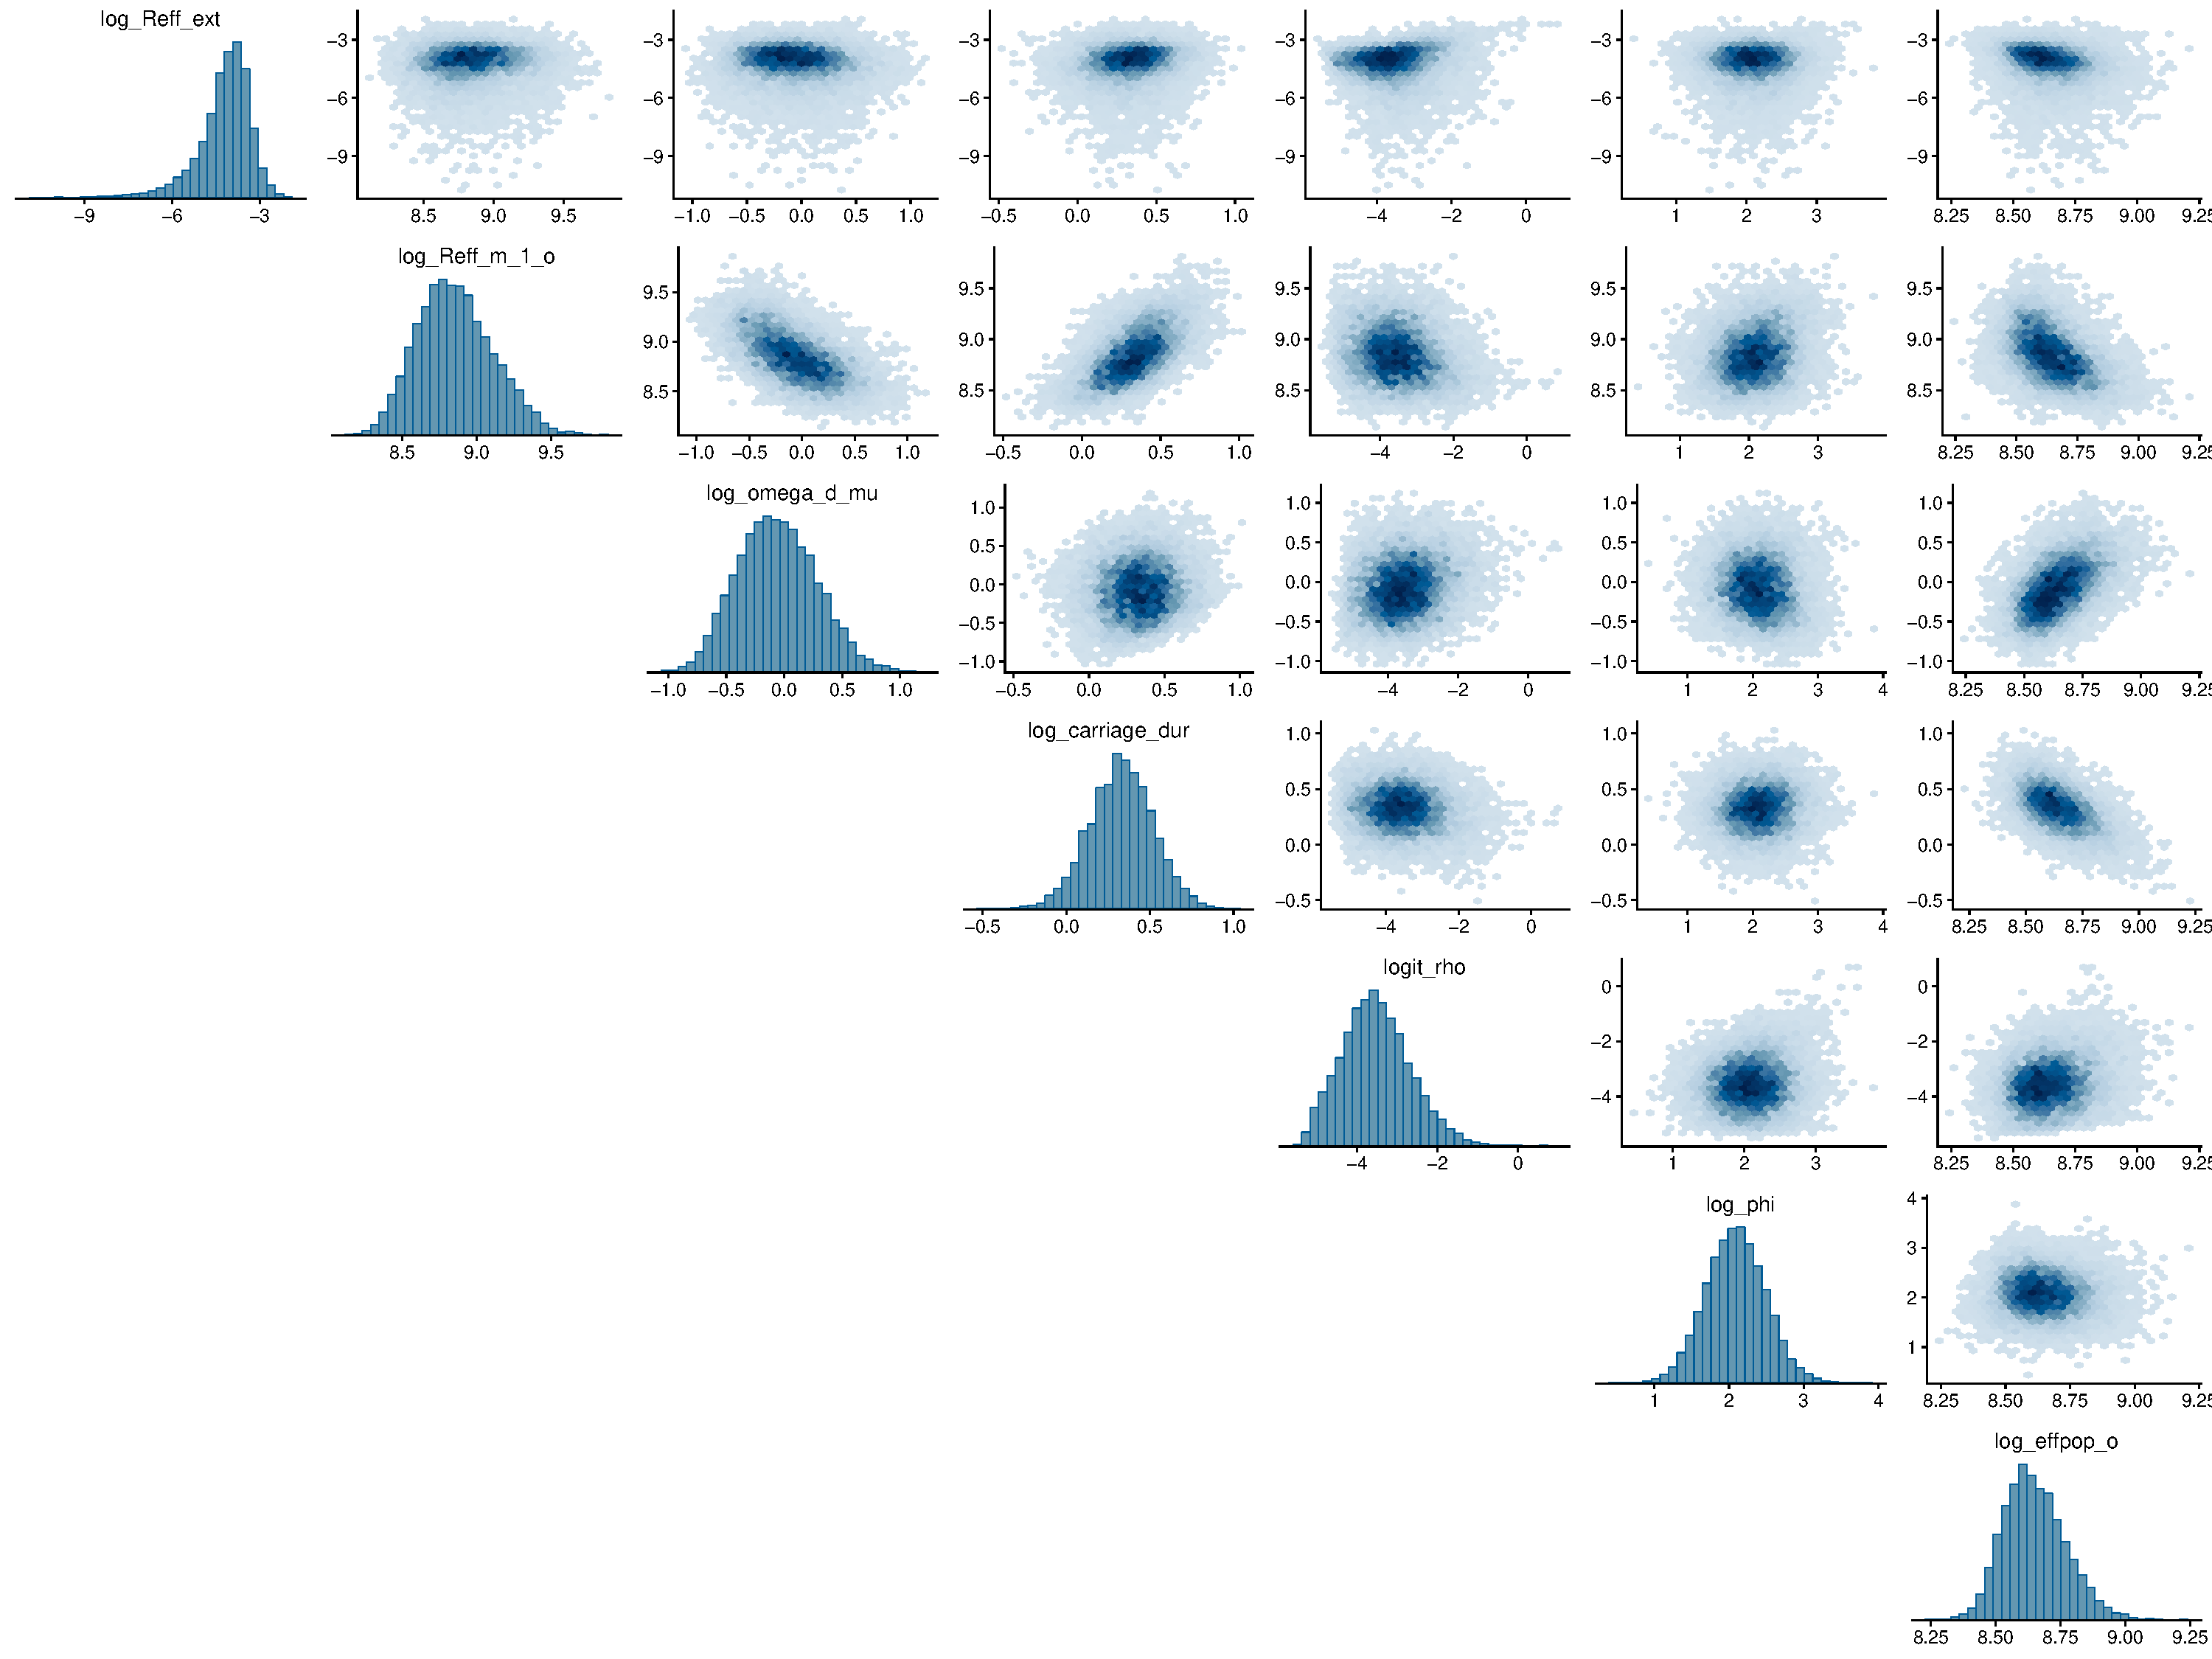
\includegraphics[width=\linewidth]{figures/lib_tight_pairs}
	\caption{Scatterplots of parameters for the SEIR model fit to data from the Ebola outbreak in Liberia.}
	\label{fig:liberiapairs}
\end{figure}

\begin{sidewaysfigure}[htbp]
	\centering
	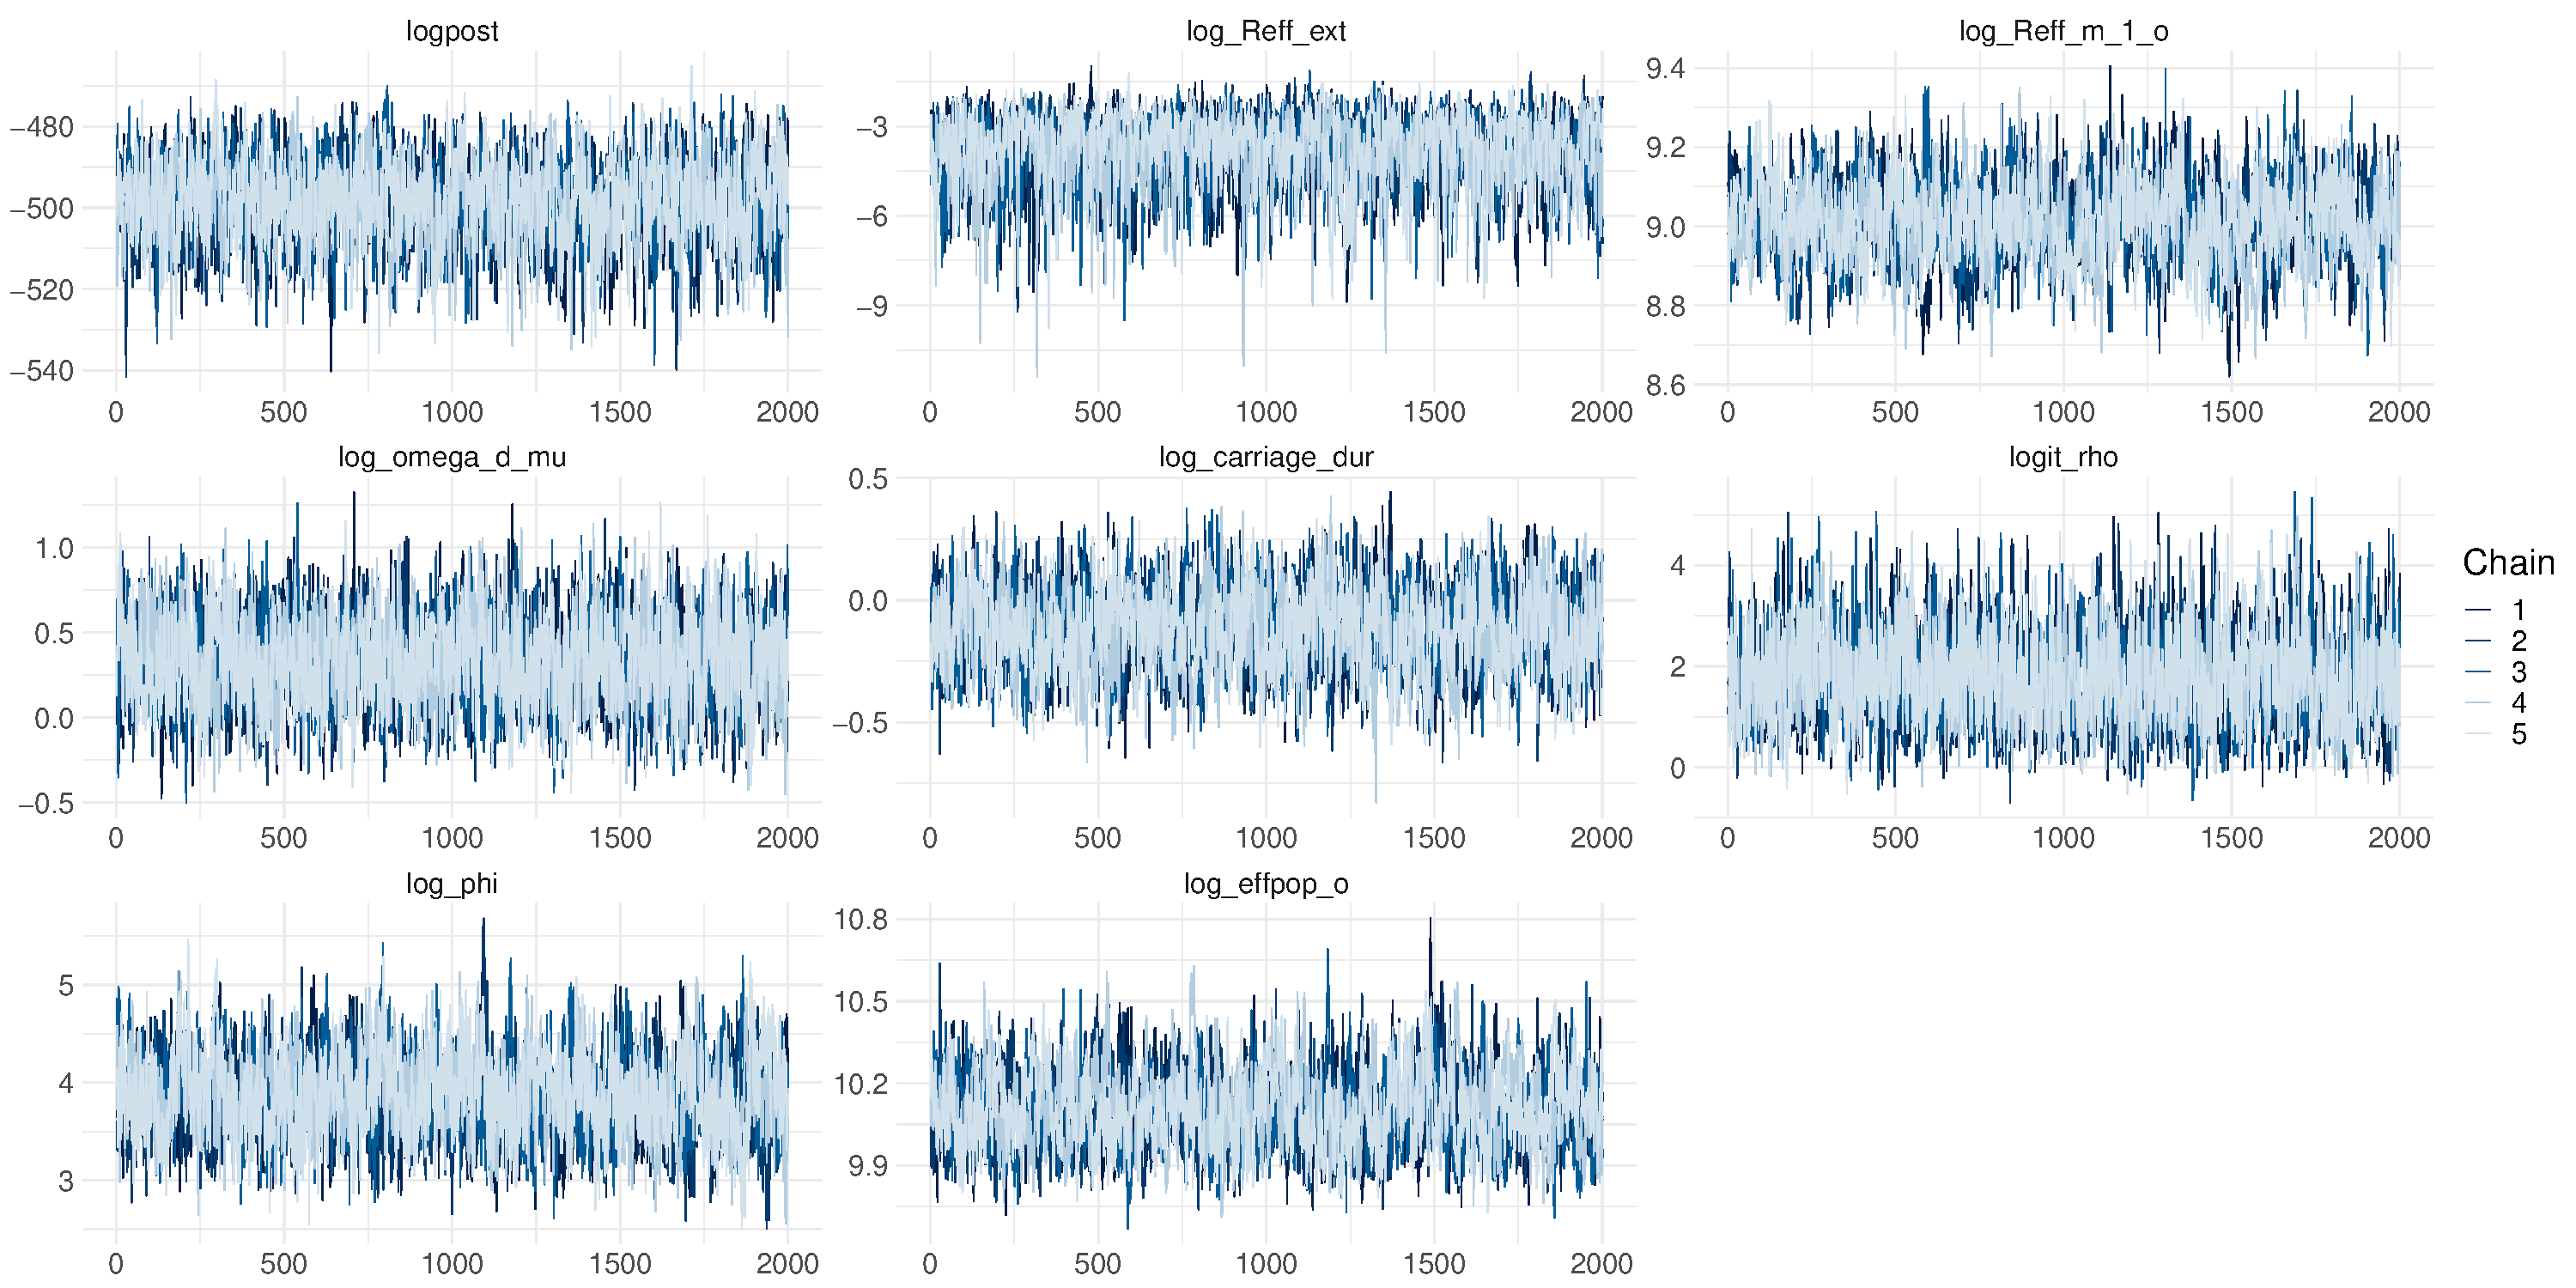
\includegraphics[width=\linewidth]{figures/sln_tight_traces}
	\caption{Posterior traceplots for the SEIR model fit to data from the Ebola outbreak in Sierra Leone.}
	\label{fig:sierraleonetraces}
\end{sidewaysfigure}

\begin{figure}[htbp]
	\centering
	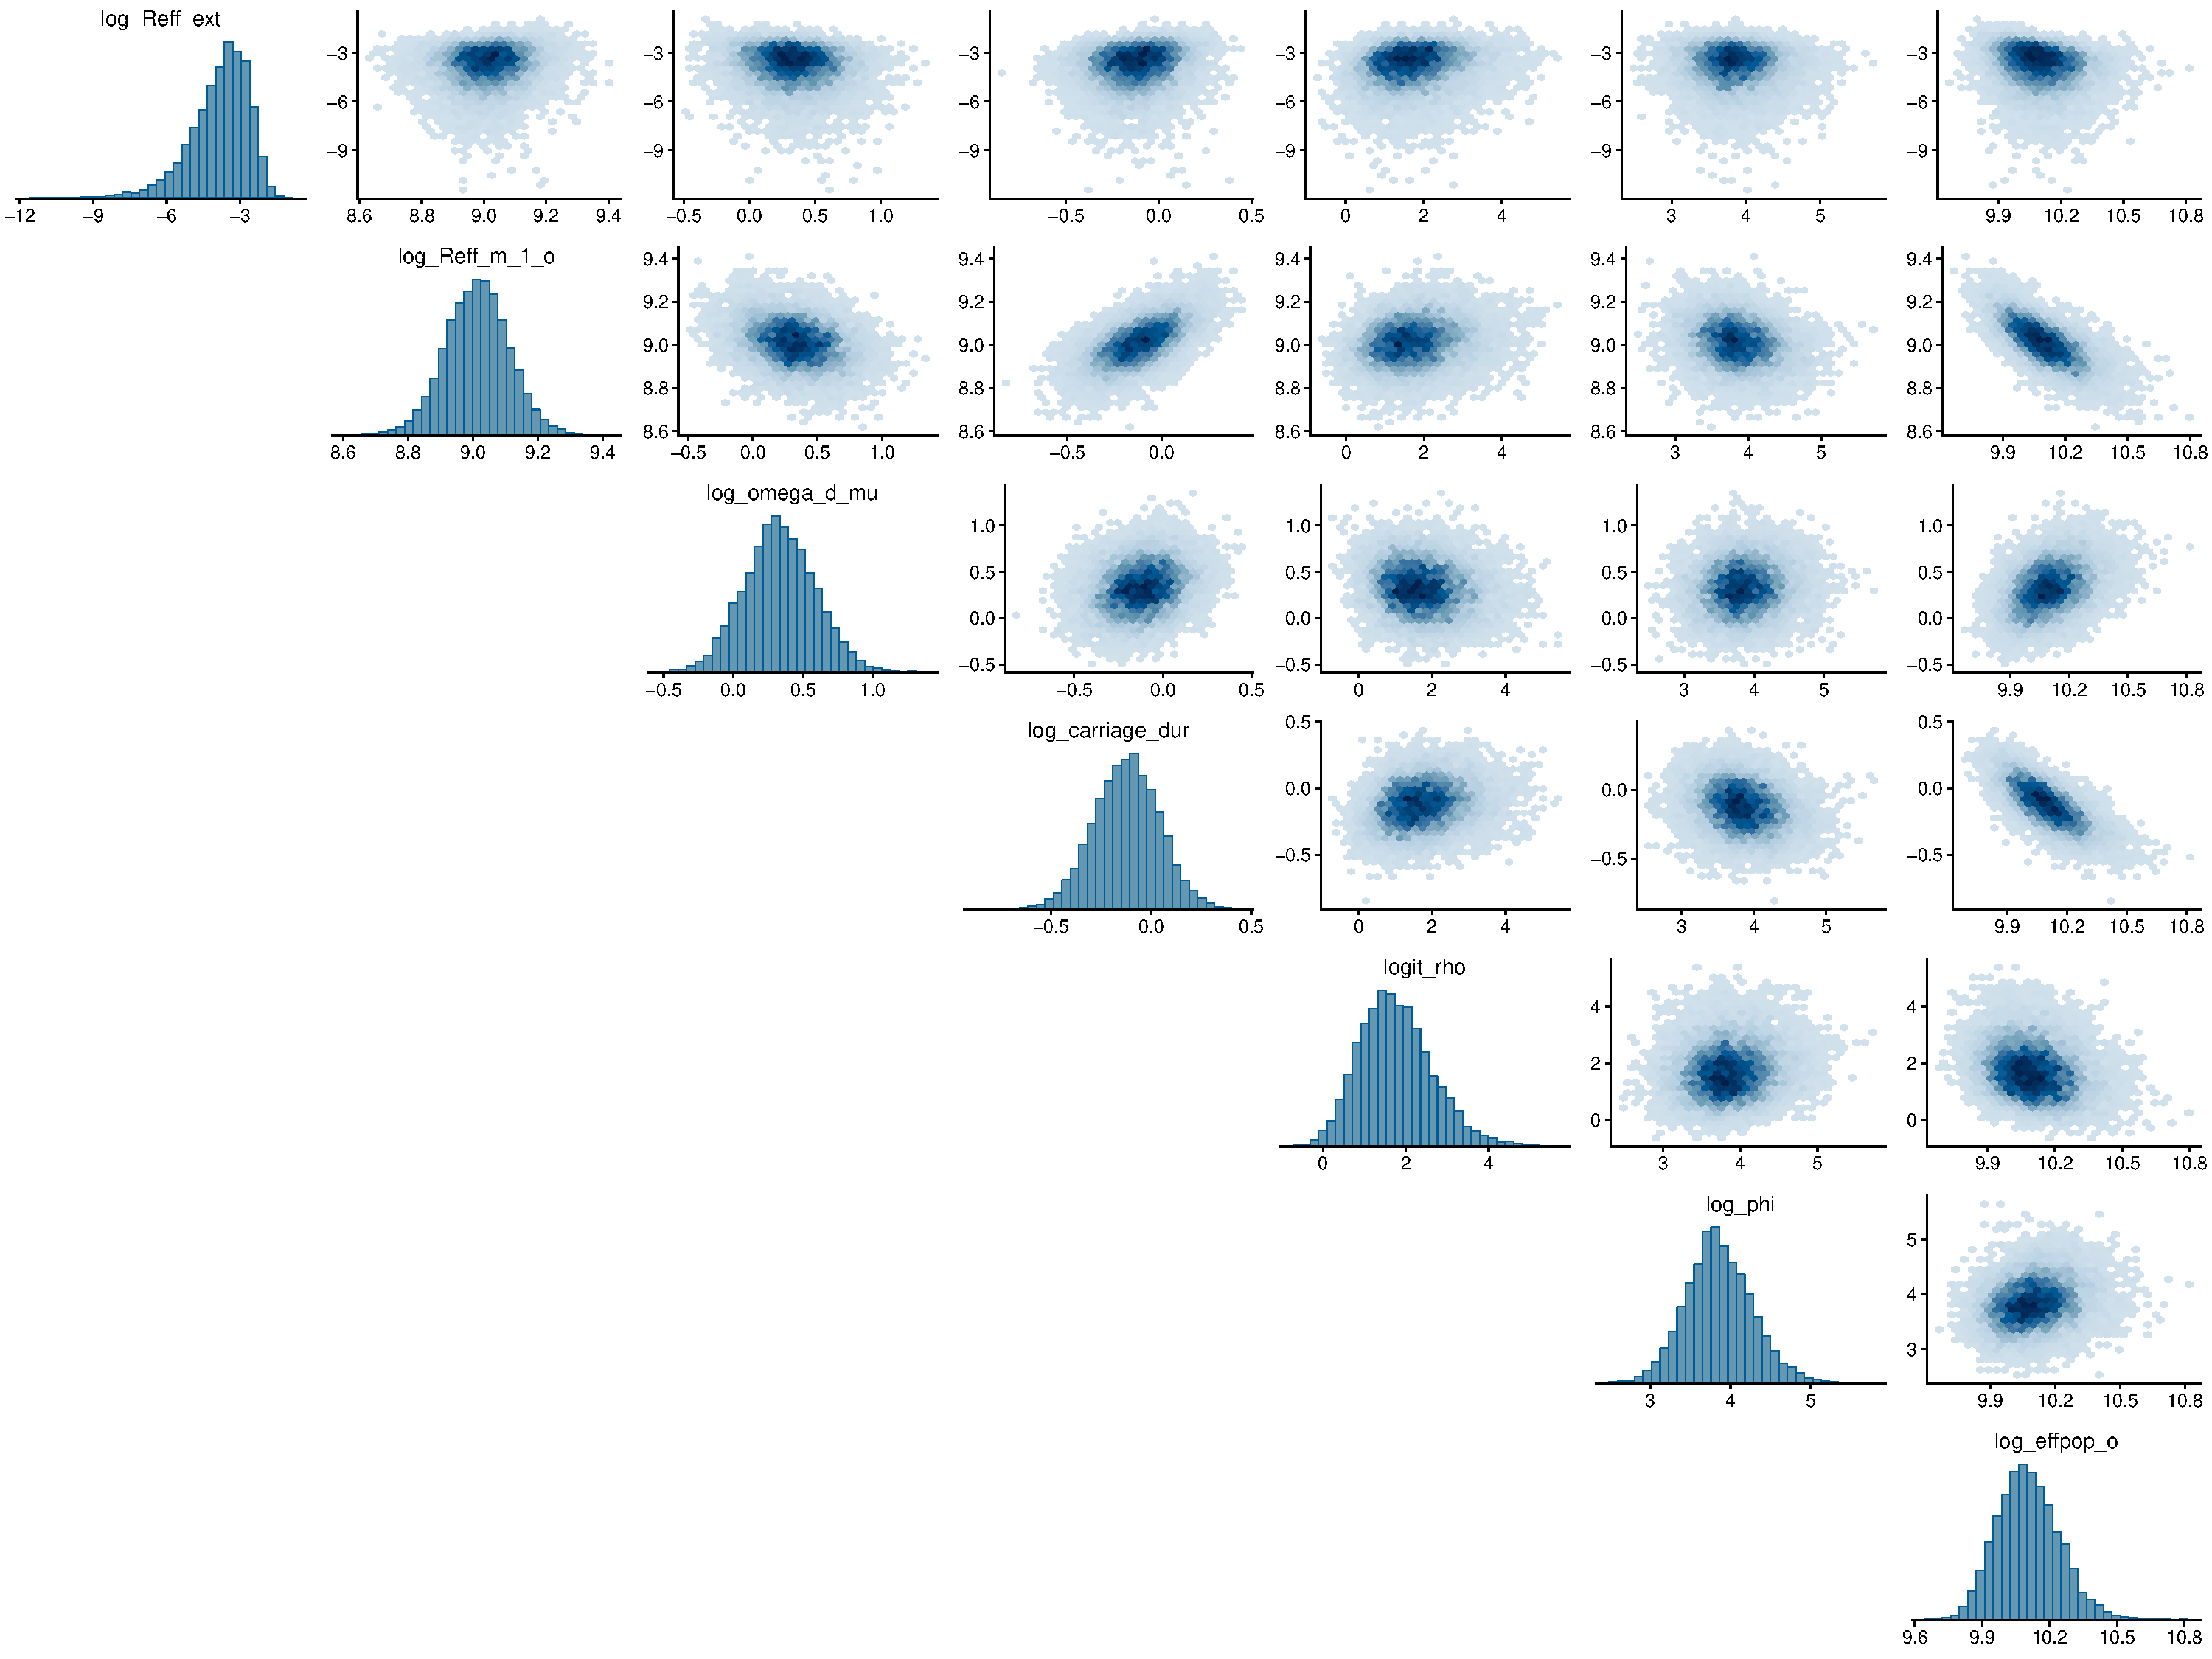
\includegraphics[width=\linewidth]{figures/sln_tight_pairs}
	\caption{Scatterplots of parameters for the SEIR model fit to data from the Ebola outbreak in Sierra Leone.}
	\label{fig:sierraleonepairs}
\end{figure}

\begin{figure}[htbp]
	\begin{fullpage}
		\centering
		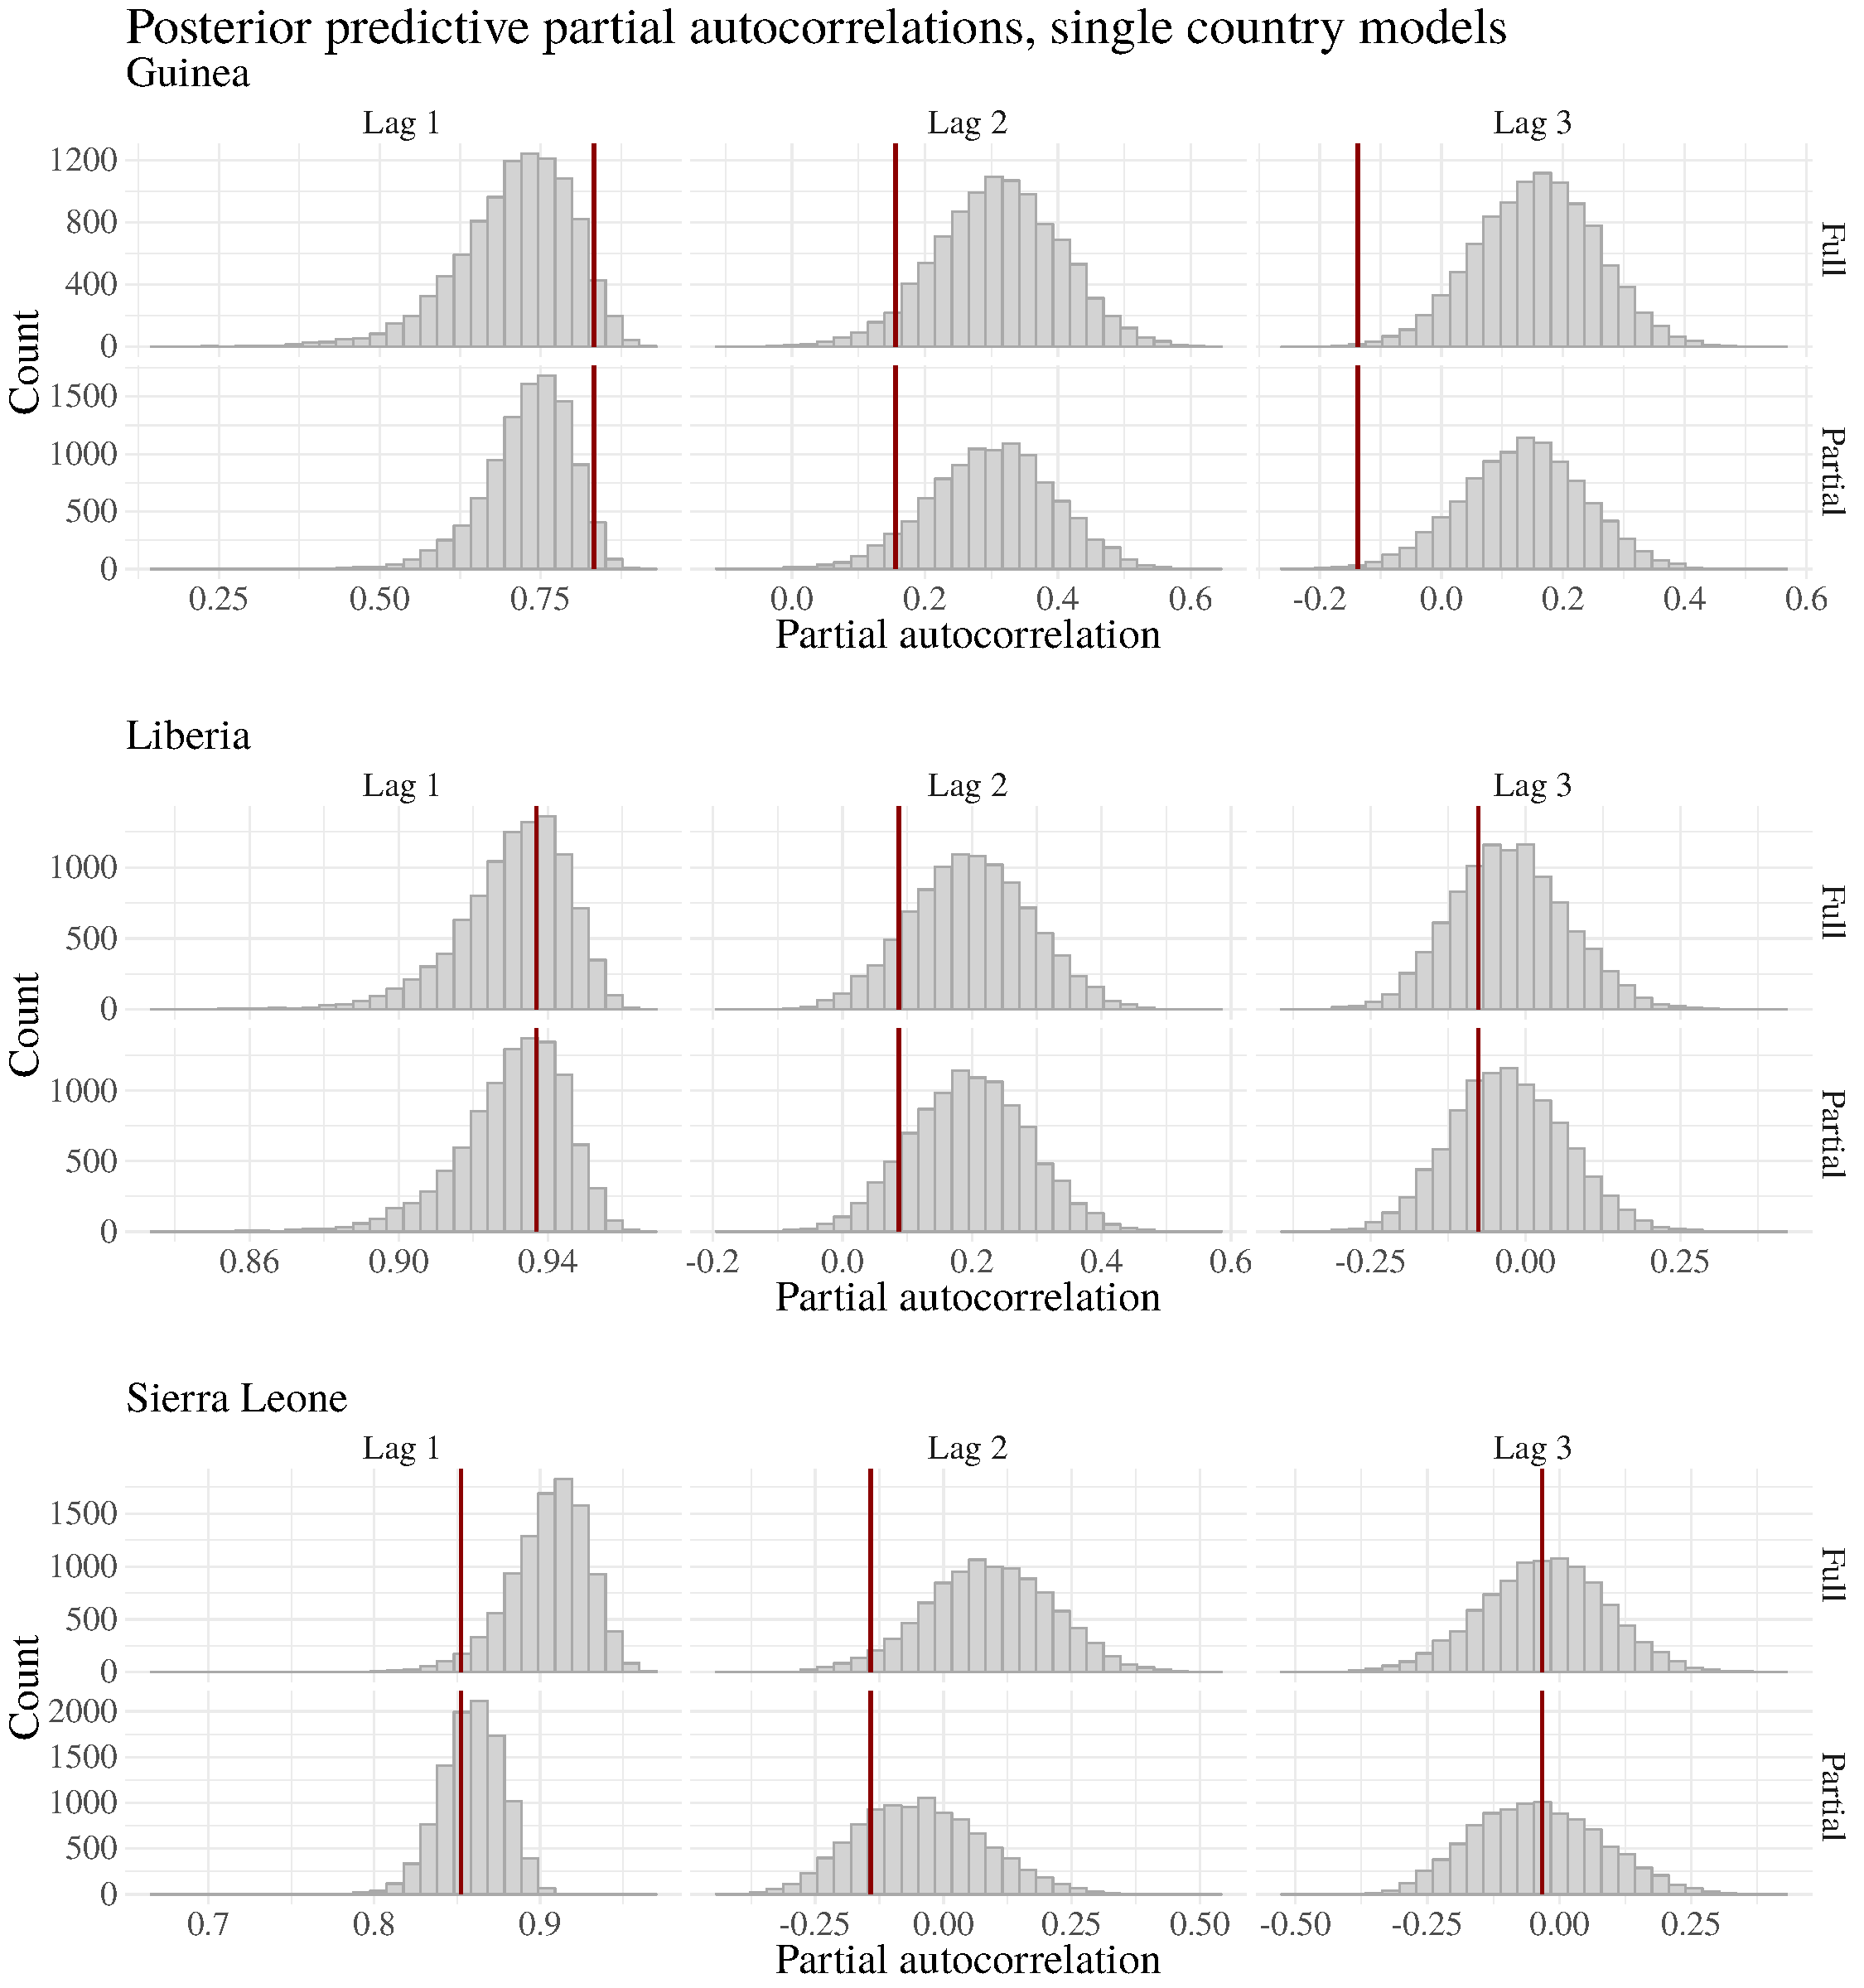
\includegraphics[width=0.8\linewidth]{figures/ebola_single_pacfs}
		\caption[Posterior predictive distributions of partial autocorrelations for the main country--specific SEIR models fit to data from the West Africa Ebola outbreak.]{Distributions of partial autocorrelations at lags 1, 2, and 3 for datasets generated under the full and partial posterior predictive distributions for the main country--specific SEIR models fit to data from the West Africa Ebola outbreak. Vertical red lines are the partial autocorrelations for the observed incidence data at the respective lags.}
		\label{fig:ebola_single_pacfs}
	\end{fullpage}
\end{figure}

\begin{sidewaysfigure}[htbp]
	\begin{fullpage}
		\centering
		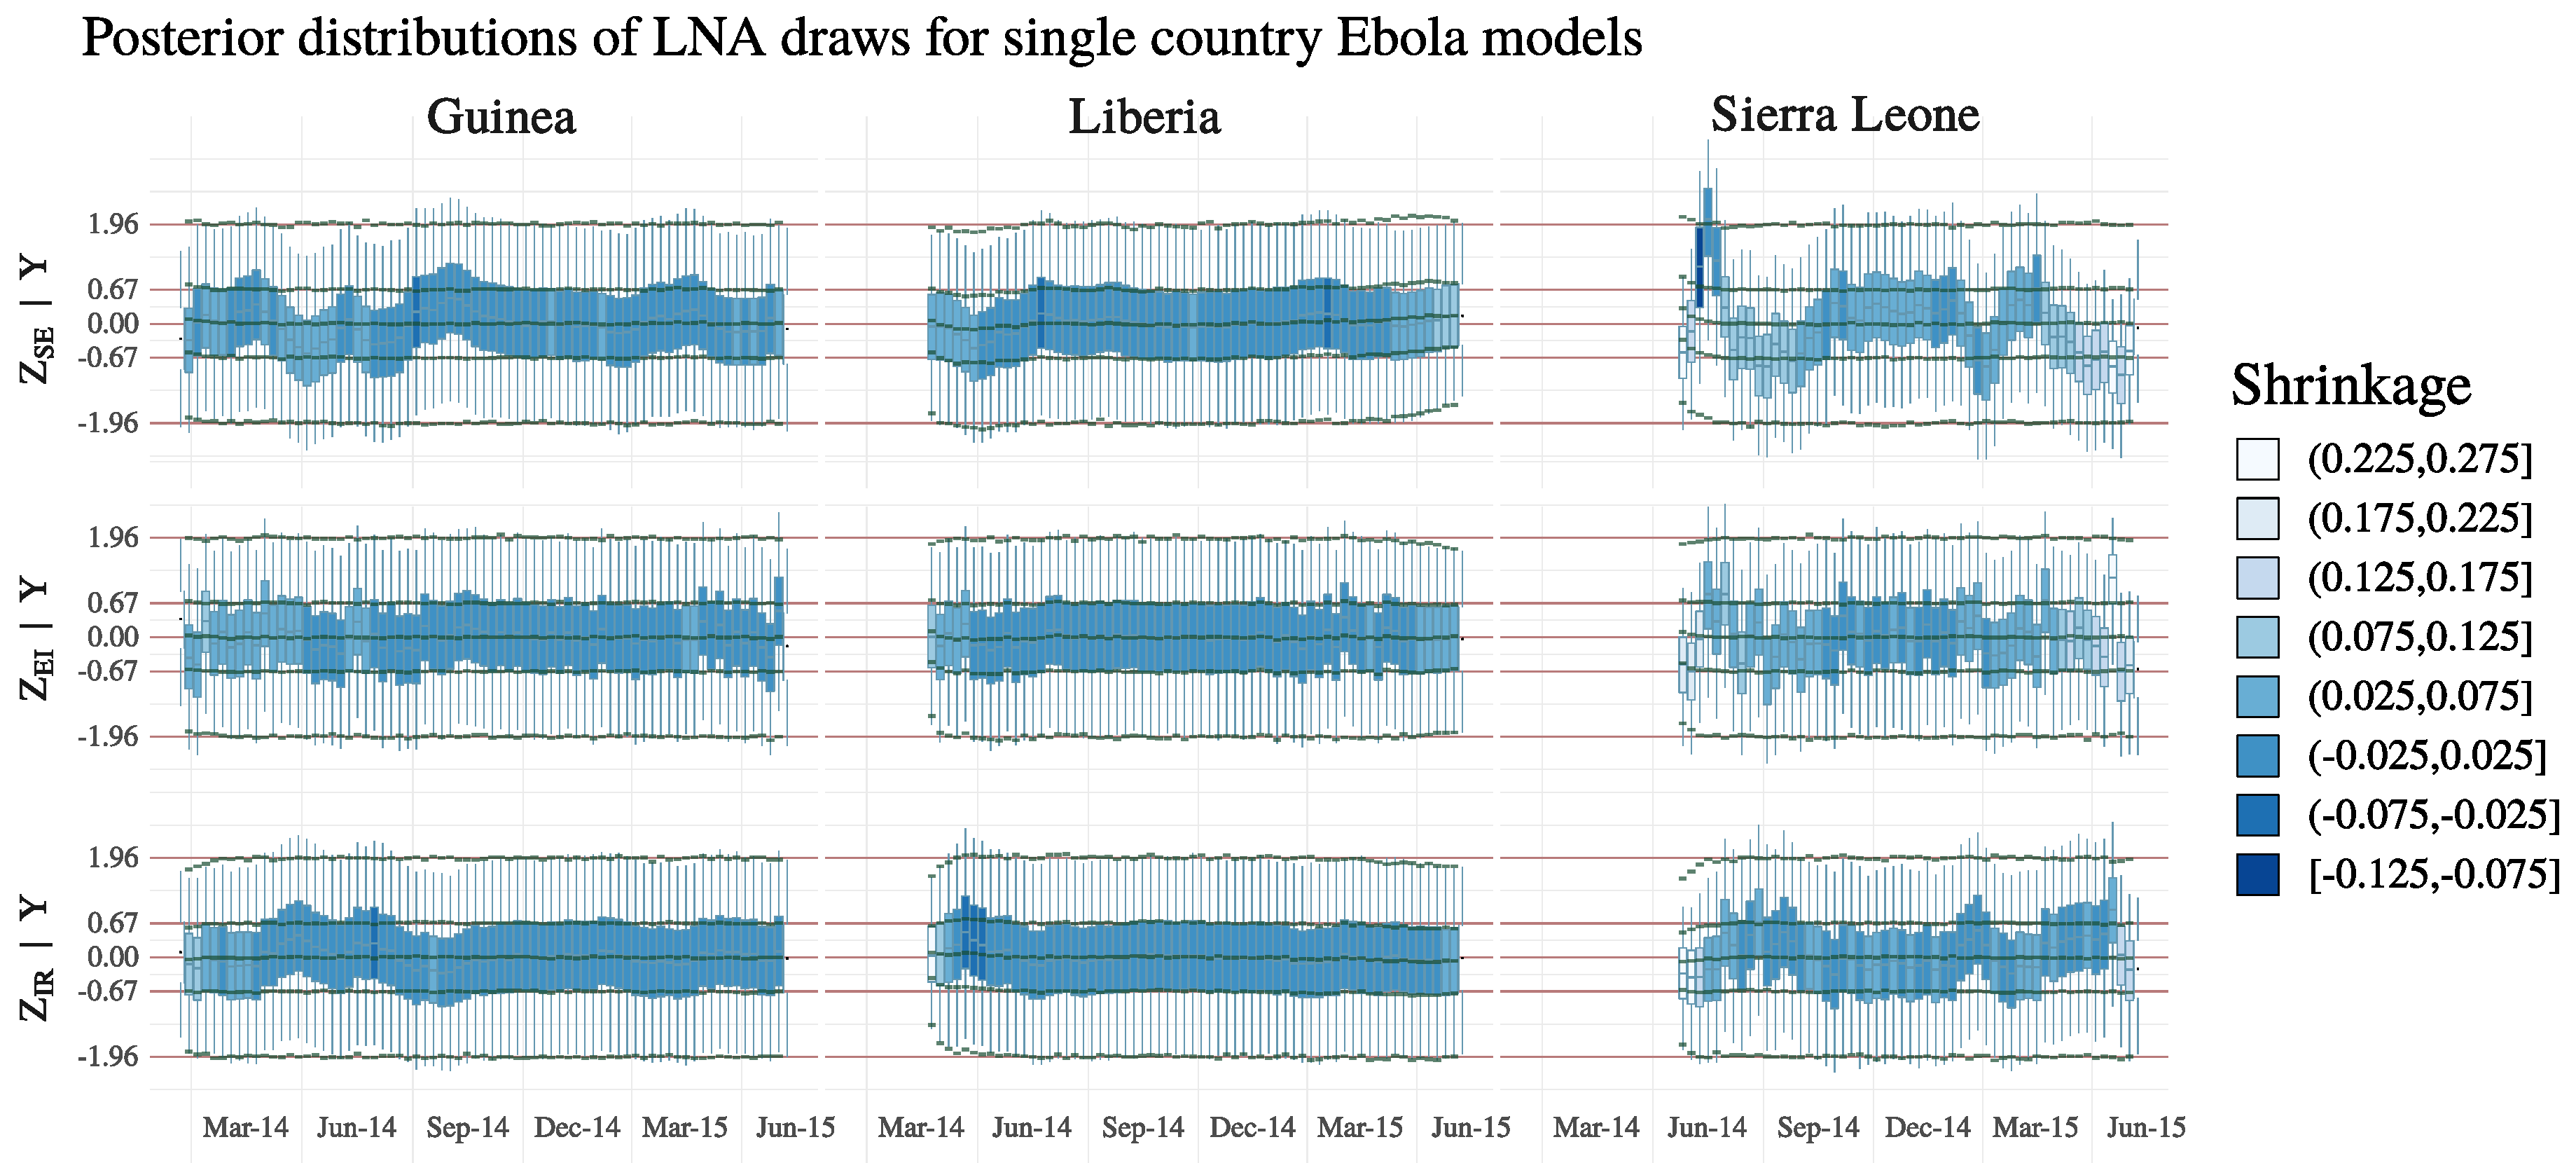
\includegraphics[width=\linewidth]{figures/ebola_single_drawplots}
		\caption[Posterior distributions of LNA draws for the main country--specific SEIR models fit to data from the West Africa Ebola outbreak.]{Posterior distributions of the LNA draws for exposures, infections, and recoveries (blue boxplots) in the main country--specific SEIR models fit data from the Ebola outbreak in Guinea, Liberia, and Sierra Leone. The lower and upper whisker tips correspond to the $ 2.5^\mr{th} $ and $ 97.5^\mr{th} $ posterior quantiles, the lower and upper hinges to the $ 25^\mr{th} $ and $ 75^\mr{th} $ quantiles, and the middle hash mark to the posterior median. The solid red lines are the theoretical quantiles of the posterior predictive distribution (or equivalently, the prior distribution) of the LNA draws, drawn at the quantiles of a standard normal distribution corresponding to the boxplot quantiles. The green ticks are the estimated quantiles of the posterior predictive distributions of the LNA draws, accounting for boundary conditions on the state space of the latent process and obtained by simulating LNA paths from the posterior predictive distribution.  The posterior distributions of LNA draws are shaded according to the level of posterior shrinkage, computed as one minus the ratio of standard deviations of LNA draws in the posterior and prior.}
		\label{fig:ebola_single_drawplots}
	\end{fullpage}
\end{sidewaysfigure}

\newpage
\subsection{Details and Supplementary Results for Multi--Country Models}
\label{subsec:ebola_joint_supplement}

\subsubsection{Priors and MCMC details}
\label{subsubsec:ebola_joint_mcmc}

We fit stratified SEIR models to the Ebola incidence data from Guinea, Liberia, and Sierra Leone under two prior regimes given in Tables \ref{tab:ebola_priors_joint_tight} and \ref{tab:ebola_priors_joint_diffuse}. Cross--border transmission was incorporated into the rate of infection via virtual migration, as explained in Section \ref{subsec:ebola_synth}.  The model fitting procedure and priors were the same for both models, and were also the same for models fit via the LNA and ODE. We ran five chains for each model, initialized at random parameter values, for 200,000 iterations per chain. The model parameters, not including the initial compartment volumes, were jointly updated via MVNSS (see Section \ref{subsubsec:mvn_slice_sampling}). The empirical covariance for the MVNSS algorithm was adapted over the first 100,000 iterations using the gain factor sequence, $\gamma_n = 0.5(1 + 0.01n)^{-0.9}$. The contribution of isotropic Gaussian noise to the proposal was initialized at 0.001 and reduced throughout the adaptation phase according to the sequence $ \iota_n = 0.001(1 + 0.01n)^{-0.99} $. The covariance matrix was blocked by country with covariances for parameters belonging to different countries set to zero. Thus, country specific parameters were proposed jointly but were independent in the proposal. Migration parameters were blocked with parameters corresponding to the destination country. The initial compartment volumes were updated jointly with the LNA paths in an EllipSS step. The MCMC alternated between three ElliptSS and two MVNSS updates per MCMC iteration. The ElliptSS bracket width was reset after the first 5,000 MCMC iterations to $ \omega = 2\sqrt{2\log(10)}\sigma_{ElliptSS}$, where $ \sigma_{ElliptSS} $ was the standard deviation of the accepted angles over the initial iterations. The MCMC estimation scales for each country were parameterized as in Table \ref{tab:seir_params_est3} with the one addition being the log ratio of effective reproductive numbers, subtract one, for Guinea, $ \log\left ((R_{eff,G}^{(2)}-1)/(R_{eff,G}^{(1)}-1)\right ) $. Convergence was assessed visually by inspection of traceplots of posterior samples, and via potential scale reduction factors (PSRFs) \cite{brooks1998general} computed via the \texttt{coda} R package \cite{codapackage}. The models each took roughly three days to run. 

\begin{table}[htbp]
	\caption[Priors for initial compartment volumes for a stratified SEIR model fit to data from the Ebola outbreak in West Africa.]{Priors for the initial compartment volumes at the times when transmission commenced in each country for single country models fit to data from the Ebola outbreak in West Africa. The initial compartment volumes for each country are assigned independent truncated multivariate normal priors that respect the boundary conditions on the state space of compartment volumes for that country (explained in Section \ref{sec:lna_init_volumes}). If the population size for country A is $ N_A $, and the initial state probability is denoted $ \bp_{0,A} = \bX_{0,A}/N_A  = (S_{0,A}, E_{0,A}, I_{0,A}, R_{0,A})/N_A$, the prior is a truncated multivariate normal approximation of a multinomial distribution with mean $ N_A\bp_{0,A}$ and covariance $ N_A(\bP_{0,A} - \bp_{0,A}\bp_{0,A}^T) $.} 
	\label{tab:ebola_joint_initdist_priors}
	\centering
	\begin{tabular}{lc}
		\hline \textbf{Country} & \textbf{Prior mean initial volumes} ($ \bX_0 $) \\
		\hline
		Guinea & ($ 11.8\times10^6 -7.1$, 4, 3, 0.1) \\
		Liberia & ($ 4.4\times10^6 -5.1$, 3, 2, 0.1) \\
		Sierra Leone & ($ 7.1\times10^6 -5.1$, 3, 2, 0.1) \\
		\hline
	\end{tabular}
\end{table}

\begin{sidewaystable}[htbp]
	\begin{fullpage}
		\caption[Parameters and priors for a country--stratified SEIR model fit to the West Africa Ebola outbreak.]{Parameters for a country--stratified SEIR model fit to the West Africa Ebola outbreak, prior distributions, 95\% prior intervals, and references that informed the choice of priors. Subscripts, $ G,L,S, $ indicate specific countries, or generic countries $ A,B $ if a prior is shared. Effective reproduction numbers are defined with respect to the effective population size as $ R_{eff} = \beta N_{eff} /\mu $.}
		\label{tab:ebola_priors_joint_tight}
		\scriptsize
		\centering
		\begin{tabular}{lllrr}
			\hline
			\textbf{Parameter} &  \textbf{Interpretation} & \textbf{Prior} & \textbf{Median (95\% Interval)} & \textbf{References} \\ \hline
			$ R_{eff,G}^{(2)} / R_{eff,G}^{(1)} $ & Ratio of effective reproduction \#s &  LogNormal(0, 0.5$ ^2 $) & $ R_{eff,G}^{(2)} / R_{eff,G}^{(1)} = $ 1.00 (0.38, 2.66) & \cite{chowell2014transmission,chretien2015mathematical,coltart2017ebola,king2015avoidable} \\
			$ R_{eff,G}^{(2)}(t)-1 $ & Effective reproduction \# - 1, $ t\geq33 $ & LogNormal(log(0.5), $ 0.75^2 $) & $ \implies R_{eff,G}^{(2)} = 1.50 (1.11, 3.17)$ &  \cite{chowell2014transmission,chretien2015mathematical,coltart2017ebola,king2015avoidable} \\
			$ R_{eff,L} -1 $ & Effective reproduction \#-1 &  LogNormal(log(0.5), $ 0.75^2 $) & $ \implies R_{eff,L} = 1.50 (1.11, 3.17)$ &  \cite{chowell2014transmission,chretien2015mathematical,coltart2017ebola,king2015avoidable} \\
			$ R_{eff,S}-1 $ & Effective reproduction \#-1 & LogNormal(log(0.5), 0.75$ ^2 $) & $ \implies R_{eff,S} = 1.50 (1.11, 3.17)$ &  \cite{chowell2014transmission,chretien2015mathematical,coltart2017ebola,king2015avoidable}\\
			\makecell[l]{$ \alpha_{GS},\alpha_{GL}, \alpha_{LG},$\\
			$ \alpha_{LS},\alpha_{SG}, \alpha_{SL} $} & \makecell[l]{Infectious migration rate \\ from country A to B} & $ 1000\alpha_{AB} \sim$ Exponential(0.25) & \makecell[r]{\# migrations per 1000 infected \\ = 2.78 (0.10, 14.76)} & \cite{dudas2017virus}\\ 
			$ \omega_G/\omega_G $ & Rate from $ E_G\rightarrow I_G $ & LogNormal(0.0, 0.3$ ^2 $) & $ (1/\mu_G)\big/(1/\omega_G) $ = 1.00 (0.56, 1.80) & \cite{chowell2014transmission,velasquez2015time,glynn2017variability} \\
			$ \omega_L/\omega_L $ & Rate from $ E_L\rightarrow I_L $ & LogNormal(0.0, 0.3$ ^2 $) & $ (1/\mu_L)\big/(1/\omega_L) $ = 1.00 (0.56, 1.80) & \cite{chowell2014transmission,velasquez2015time,glynn2017variability} \\
			$ \omega_S/\omega_S $ & Rate from $ E_S\rightarrow I_S $ & LogNormal(0.0, 0.3$ ^2 $) & $ (1/\mu_S)\big/(1/\omega_S) $ = 1.00 (0.56, 1.80) & \cite{chowell2014transmission,velasquez2015time,glynn2017variability} \\
			$ 1/\mu_G $ & Rate from $ E_G\rightarrow I_G $ &  LogNormal(0.3, 0.2$ ^2 $) & $ 7/\mu_G = $ 9.45 (6.38, 13.98) & \cite{chowell2014transmission,velasquez2015time,glynn2017variability} \\
			$ 1/\mu_L $ & Rate from $ E_L\rightarrow I_L $ &  LogNormal(0.3, 0.2$ ^2 $) & $ 7/\mu_L = $ 9.45 (6.38, 13.98) & \cite{chowell2014transmission,velasquez2015time,glynn2017variability} \\
			$ 1/\mu_S $ & Rate from $ E_S\rightarrow I_S $ &  LogNormal(0.3, 0.2$ ^2 $) & $ 7/\mu_S = $ 9.45 (6.38, 13.98) & \cite{chowell2014transmission,velasquez2015time,glynn2017variability} \\
			$ N_{eff,G} $ & Effective population size & $\mr{Unif}(\sum_{\ell=1}^{L}Y_\ell^G, N_G/4) $& $ N_{eff,G} \in (3627,\ 2.95\times10^6) $ & Scale of counts \\
			$ N_{eff,L} $ & Effective population size & $\mr{Unif}(\sum_{\ell=1}^{L}Y_\ell^L, N_L/4) $& $ N_{eff,L} \in (4994,\ 1.1\times10^6) $ & Scale of counts \\
			$ N_{eff,S} $ & Effective population size & $\mr{Unif}(\sum_{\ell=1}^{L}Y_\ell^S, N_S/4) $& $ N_{eff,S} \in (11317,\ 1.775\times10^6) $ & Scale of counts \\
			$ \rho_G $ &  Mean case detection prob. & LogitNormal(0, 1.4$ ^2 $) & $ \implies \rho_G = 0.5, (0.06, 0.94)$ & Very high and very low $ \rho $ unlikely. \\
			$ \rho_L $ &  Mean case detection prob. & LogitNormal(0, 1.4$ ^2 $) & $ \implies \rho_L = 0.5, (0.06, 0.94)$ & Very high and very low $ \rho $ unlikely. \\
			$ \rho_S $ & Mean case detection prob. & LogitNormal(0, 1.4$ ^2 $) & $ \implies \rho_S = 0.5, (0.06, 0.94)$ & Very high and very low $ \rho $ unlikely. \\
			$ \phi_G,\ \phi_L, \phi_S $ &  Neg.Binomial overdispersion & LogNormal(0, 5$ ^2 $) & $ \implies \ = 1, (5.5\times 10^-5, 1.8\times10^4)$ & Diffuse. \\
			\hline
		\end{tabular}
	\end{fullpage}
\end{sidewaystable}

\begin{sidewaystable}[htbp]
	\begin{fullpage}
		\caption[Loose priors used in a sensitivity analysis for a stratified SEIR model for Ebola in West Africa.]{Priors for a sensitivity analysis for the country--stratified SEIR model fit to the West Africa Ebola outbreak. Priors were less informative priors for the effective reproductive numbers, cross--border transmission, and infectious period duration vis--a--vis the main model. Subscripts, $ G,L,S, $ indicate specific countries, or generic countries $ A,B $ if a prior is shared. Effective reproduction numbers are defined with respect to the effective population size as $ R_{eff} = \beta N_{eff} /\mu $.}
		\label{tab:ebola_priors_joint_diffuse}
		\scriptsize
		\centering
		\begin{tabular}{lllrr}
			\hline
			\textbf{Parameter} &  \textbf{Interpretation} & \textbf{Prior} & \textbf{Median (95\% Interval)} & \textbf{References} \\ \hline
			$ R_{eff,G}^{(2)} / R_{eff,G}^{(1)} $ & Ratio of effective reproduction \#s &  LogNormal(0, 0.5$ ^2 $) & $ R_{eff,G}^{(2)} / R_{eff,G}^{(1)} = $ 1.00 (0.38, 2.66) & \cite{chowell2014transmission,chretien2015mathematical,coltart2017ebola,king2015avoidable} \\
			$ R_{eff,G}^{(2)}(t)-1 $ & Effective reproduction \# - 1, $ t\geq33 $ & LogNormal(log(0.5), $ 1.5^2 $) & $ \implies R_{eff,G}^{(2)} = 1.50 (1.02, 10.46)$ &  \cite{chowell2014transmission,chretien2015mathematical,coltart2017ebola,king2015avoidable} \\
			$ R_{eff,L} -1 $ & Effective reproduction \#-1 &  LogNormal(log(0.5), $ 1.5^2 $) & $ \implies R_{eff,L} = 1.50 (1.02, 10.46)$ &  \cite{chowell2014transmission,chretien2015mathematical,coltart2017ebola,king2015avoidable} \\
			$ R_{eff,S}-1 $ & Effective reproduction \#-1 & LogNormal(log(0.5), 1.5$ ^2 $) & $ \implies R_{eff,S} = 1.50 (1.02, 10.46)$ &  \cite{chowell2014transmission,chretien2015mathematical,coltart2017ebola,king2015avoidable}\\
			\makecell[l]{$ \alpha_{GS},\alpha_{GL}, \alpha_{LG},$\\
				$ \alpha_{LS},\alpha_{SG}, \alpha_{SL} $} & \makecell[l]{Infectious migration rate \\ from country A to B} & $ 1000\alpha_{AB} \sim$ Exponential(0.125) & \makecell[r]{\# migrations per 1000 infected \\ = 5.55 (0.20, 29.51)} & \cite{dudas2017virus}\\ 
			$ \omega_G/\omega_G $ & Rate from $ E_G\rightarrow I_G $ & LogNormal(0.0, 0.3$ ^2 $) & $ (1/\mu_G)\big/(1/\omega_G) $ = 1.00 (0.56, 1.80) & \cite{chowell2014transmission,velasquez2015time,glynn2017variability} \\
			$ \omega_L/\omega_L $ & Rate from $ E_L\rightarrow I_L $ & LogNormal(0.0, 0.3$ ^2 $) & $ (1/\mu_L)\big/(1/\omega_L) $ = 1.00 (0.56, 1.80) & \cite{chowell2014transmission,velasquez2015time,glynn2017variability} \\
			$ \omega_S/\omega_S $ & Rate from $ E_S\rightarrow I_S $ & LogNormal(0.0, 0.3$ ^2 $) & $ (1/\mu_S)\big/(1/\omega_S) $ = 1.00 (0.56, 1.80) & \cite{chowell2014transmission,velasquez2015time,glynn2017variability} \\
			$ 1/\mu_G $ & Rate from $ E_G\rightarrow I_G $ &  LogNormal(0.3, 0.35$ ^2 $) & $ 7/\mu_G = $ 9.45 (4.76, 18.76) & \cite{chowell2014transmission,velasquez2015time,glynn2017variability} \\
			$ 1/\mu_L $ & Rate from $ E_L\rightarrow I_L $ &  LogNormal(0.3, 0.35$ ^2 $) & $ 7/\mu_L = $ 9.45 (4.76, 18.76) & \cite{chowell2014transmission,velasquez2015time,glynn2017variability} \\
			$ 1/\mu_S $ & Rate from $ E_S\rightarrow I_S $ &  LogNormal(0.3, 0.35$ ^2 $) & $ 7/\mu_S = $ 9.45 (4.76, 18.76) & \cite{chowell2014transmission,velasquez2015time,glynn2017variability} \\
			$ N_{eff,G} $ & Effective population size & $\mr{Unif}(\sum_{\ell=1}^{L}Y_\ell^G, N_G/4) $& $ N_{eff,G} \in (3627,\ 2.95\times10^6) $ & Scale of counts \\
			$ N_{eff,L} $ & Effective population size & $\mr{Unif}(\sum_{\ell=1}^{L}Y_\ell^L, N_L/4) $& $ N_{eff,L} \in (4994,\ 1.1\times10^6) $ & Scale of counts \\
			$ N_{eff,S} $ & Effective population size & $\mr{Unif}(\sum_{\ell=1}^{L}Y_\ell^S, N_S/4) $& $ N_{eff,S} \in (11317,\ 1.775\times10^6) $ & Scale of counts \\
			$ \rho_G $ &  Mean case detection prob. & LogitNormal(0, 1.4$ ^2 $) & $ \implies \rho_G = 0.5, (0.06, 0.94)$ & Very high and very low $ \rho $ unlikely. \\
			$ \rho_L $ &  Mean case detection prob. & LogitNormal(0, 1.4$ ^2 $) & $ \implies \rho_L = 0.5, (0.06, 0.94)$ & Very high and very low $ \rho $ unlikely. \\
			$ \rho_S $ & Mean case detection prob. & LogitNormal(0, 1.4$ ^2 $) & $ \implies \rho_S = 0.5, (0.06, 0.94)$ & Very high and very low $ \rho $ unlikely. \\
			$ \phi_G,\ \phi_L, \phi_S $ &  Neg.Binomial overdispersion & LogNormal(0, 5$ ^2 $) & $ \implies \ = 1, (5.5\times 10^-5, 1.8\times10^4)$ & Diffuse. \\
			\hline
		\end{tabular}
	\end{fullpage}
\end{sidewaystable}

\subsubsection{Additional results}
\label{subsubsec:ebola_joint_supp_res}

\begin{table}[htbp]
	\caption[Posterior estimates of initial numbers of exposed, infected, and recovered individuals for a stratified SEIR model fit to Ebola outbreak data.]{Posterior estimates of initial numbers of exposed, infected, and recovered individuals for the main stratified approximate SEIR model with virtual migration of infecteds fit to Ebola data from the West Africa outbreak under tight priors. The effective number of susceptibles is equal to the effective population size, reported in Table \ref{tab:ebola_joint_ests}, minus the numbers of exposed, infected, and recovered individuals, but is not reported since the effective population size is not marginally identifiable.}
	\label{tab:ebola_joint_initdist_res}
	\centering
	\begin{tabular}{ll}
		\hline
		\textbf{Parameter} & \textbf{Estimate }\\ 
		\hline
		$ E_{0,G} $&  4.3 (1.1, 7.8) \\ 
		$ E_{0,L} $&  3.4 (0.59, 6.6) \\ 
		$ E_{0,S} $&  2.3 (0.23, 5.5) \\ 
		$ I_{0,G} $& 3.4 (0.59, 6.6) \\ 
		$ I_{0,L} $&  2.6 (0.47, 5.1) \\ 
		$ I_{0,S} $& 2.4 (0.37, 4.8) \\ 
		$ R_{0,G} $& 0.1 (0.07, 0.2) \\ 
		$ R_{0,L} $&  0.1 (0.07, 0.2) \\ 
		$ R_{0,S} $&  0.1 (0.06, 0.2) \\ 
		\hline
	\end{tabular}
\end{table}

\begin{table}[htbp]
	\caption[Posterior parameter estimates for stratified SEIR models fit Ebola outbreak data.]{Posterior medians (95\% Bayesian credible intervals) for parameters of the approximate (Figure \ref{fig:stratified_seir_approx_diag}) stratified SEIR models fit to Ebola outbreak data. Subscripts, $ G,L,S, $ indicate specific countries, or generic countries $ A,B $. Effective reproduction numbers are defined with respect to the effective population size as $ R_{eff} = \beta N_{eff} /\mu $. Parameter interpretations and priors are given in Tables \ref{tab:ebola_priors_joint_tight} and \ref{tab:ebola_priors_joint_diffuse}. The more informative of the two prior regimes was presented as the main model in Section \ref{subsubsec:ebola_joint_model}.}
	\label{tab:ebola_joint_ests}
	\centering\footnotesize
	\begin{tabular}{crr}
		\hline
		& \multicolumn{2}{c}{\textbf{Posterior median (95\% BCI)}}\\\cline{2-3}
		\textbf{Parameter} & \textit{Tight Priors} & \textit{Loose Priors} \\ 
		\hline
		$ R_{eff,G}^{(1)} $& 1.1 (1, 1.3) & 1.1 (1, 1.2) \\ 
		$ R_{eff,G}^{(2)} $& 1.2 (1.1, 1.4) & 1.1 (1, 1.3) \\ 
		$ R_{eff,L} $& 2.1 (1.6, 3.3) & 1.8 (1.3, 3.4) \\ 
		$ R_{eff,S} $& 1.3 (1.1, 1.4) & 1.1 (1, 1.3) \\ 
		$ 7/\omega_G $& 7.5 (3.9, 13.6) & 5.6 (2.6, 11.4) \\ 
		$ 7/\omega_L $& 9 (4.1, 19.9) & 7.2 (2.5, 19.3) \\ 
		$ 7/\omega_S $& 4.1 (2.4, 6.6) & 3 (1.5, 5.4) \\ 
		$ 7/\mu_G $& 8.4 (5.9, 11.8) & 6.4 (3.6, 10.8) \\ 
		$ 7/\mu_L $& 9 (6, 13.2) & 7.5 (3.4, 15.5) \\ 
		$ 7/\mu_S $& 6.1 (4.4, 8.2) & 3.9 (2.4, 6.2) \\ 
		$ 1000\alpha_{GL} $& 3.0 (0.1, 15.5) & 6.3 (0.3, 29.8) \\ 
		$ 1000\alpha_{GS} $& 2.6 (0.1, 13.5) & 4.4 (0.2, 23.5) \\ 
		$ 1000\alpha_{LG} $& 3.9 (0.5, 14.2) & 6.5 (1, 20.5) \\ 
		$ 1000\alpha_{LS} $& 1.4 (0.1, 7.2) & 3 (0.2, 13.3) \\ 
		$ 1000\alpha_{SG} $& 2.6 (0.1, 13.4) & 4.7 (0.3, 25) \\ 
		$ 1000\alpha_{SL} $& 3.0 (0.1, 16.7) & 6.8 (0.2, 37.8) \\ 
		$ \rho_GN_{eff,G} $& 9900 (6600, 15600) & 14600 (7800, 29100) \\ 
		$ \rho_{L}N_{eff,L} $& 5900 (4800, 7900) & 6400 (4800, 11100) \\ 
		$ \rho_SN_{eff,S} $& 26800 (20600, 38700) & 39400 (24800, 85800) \\ 
		$ \phi_G $& 5.7 (3.4, 10.6) & 6.3 (3.6, 12.9) \\ 
		$ \phi_L $& 8.8 (4.1, 19.3) & 10.2 (4.7, 27.2) \\ 
		$ \phi_S $& 48 (22, 118) & 56 (25, 140) \\ 
		\hline
	\end{tabular}
\end{table}

\begin{table}[htbp]
	\caption{Effective sample sizes and potential scale reduction factors for the main stratified SEIR model with virtual migration of infecteds fit to data from the West Africa Ebola outbreak under tight priors.}
	\centering\footnotesize
	\begin{tabular}{lrr}
		\hline
		\textbf{Parameter} & \textbf{ESS} & \textbf{PSRF} \\ 
		\hline
		$ \log(R_{eff,G}^{(2)}/R_{eff,G}^{(1)}) $& 647 & 1.00 \\ 
		$ \log(R_{eff,G}^{(2)}) $& 626 & 1.01 \\ 
		$ \log(R_{eff,L}) $& 347 & 1.02 \\ 
		$ \log(R_{eff,S}) $& 459 & 1.08 \\ 
		$ \log(\omega_G/\mu_G) $& 1161 & 1.01 \\ 
		$ \log(\omega_L/\mu_L) $& 409 & 1.02 \\ 
		$ \log(\omega_S/\mu_S) $& 1217 & 1.01 \\ 
		$ \log(1/\mu_G) $& 1141 & 1.01 \\ 
		$ \log(1/\mu_L) $& 743 & 1.00 \\ 
		$ \log(1/\mu_S) $& 874 & 1.00 \\ 
		$ \log(1000\alpha_{GL}) $& 1583 & 1.00 \\ 
		$ \log(1000\alpha_{GS}) $& 972 & 1.02 \\ 
		$ \log(1000\alpha_{LG}) $& 292 & 1.04 \\ 
		$ \log(1000\alpha_{LS}) $& 478 & 1.02 \\ 
		$ \log(1000\alpha_{SG}) $& 1238 & 1.00 \\ 
		$ \log(1000\alpha_{SL}) $& 1198 & 1.06 \\ 
		$ \log(\rho_GN_{eff,G}) $& 725 & 1.00 \\ 
		$ \log(\rho_LN_{eff,L}) $& 521 & 1.01 \\ 
		$ \log(\rho_SN_{eff,S}) $& 479 & 1.04 \\ 
		$ \logit(\rho_G) $& 631 & 1.01 \\ 
		$ \logit(\rho_L) $& 217 & 1.04 \\ 
		$ \logit(\rho_S) $& 1414 & 1.01 \\ 
		$ \log(\phi_G) $& 596 & 1.03 \\ 
		$ \log(\phi_L) $& 1098 & 1.01 \\ 
		$ \log(\phi_S) $& 489 & 1.00 \\ 
		\hline
	\end{tabular}
\end{table}

\begin{sidewaysfigure}[htbp]
	\begin{fullpage}
		\centering
		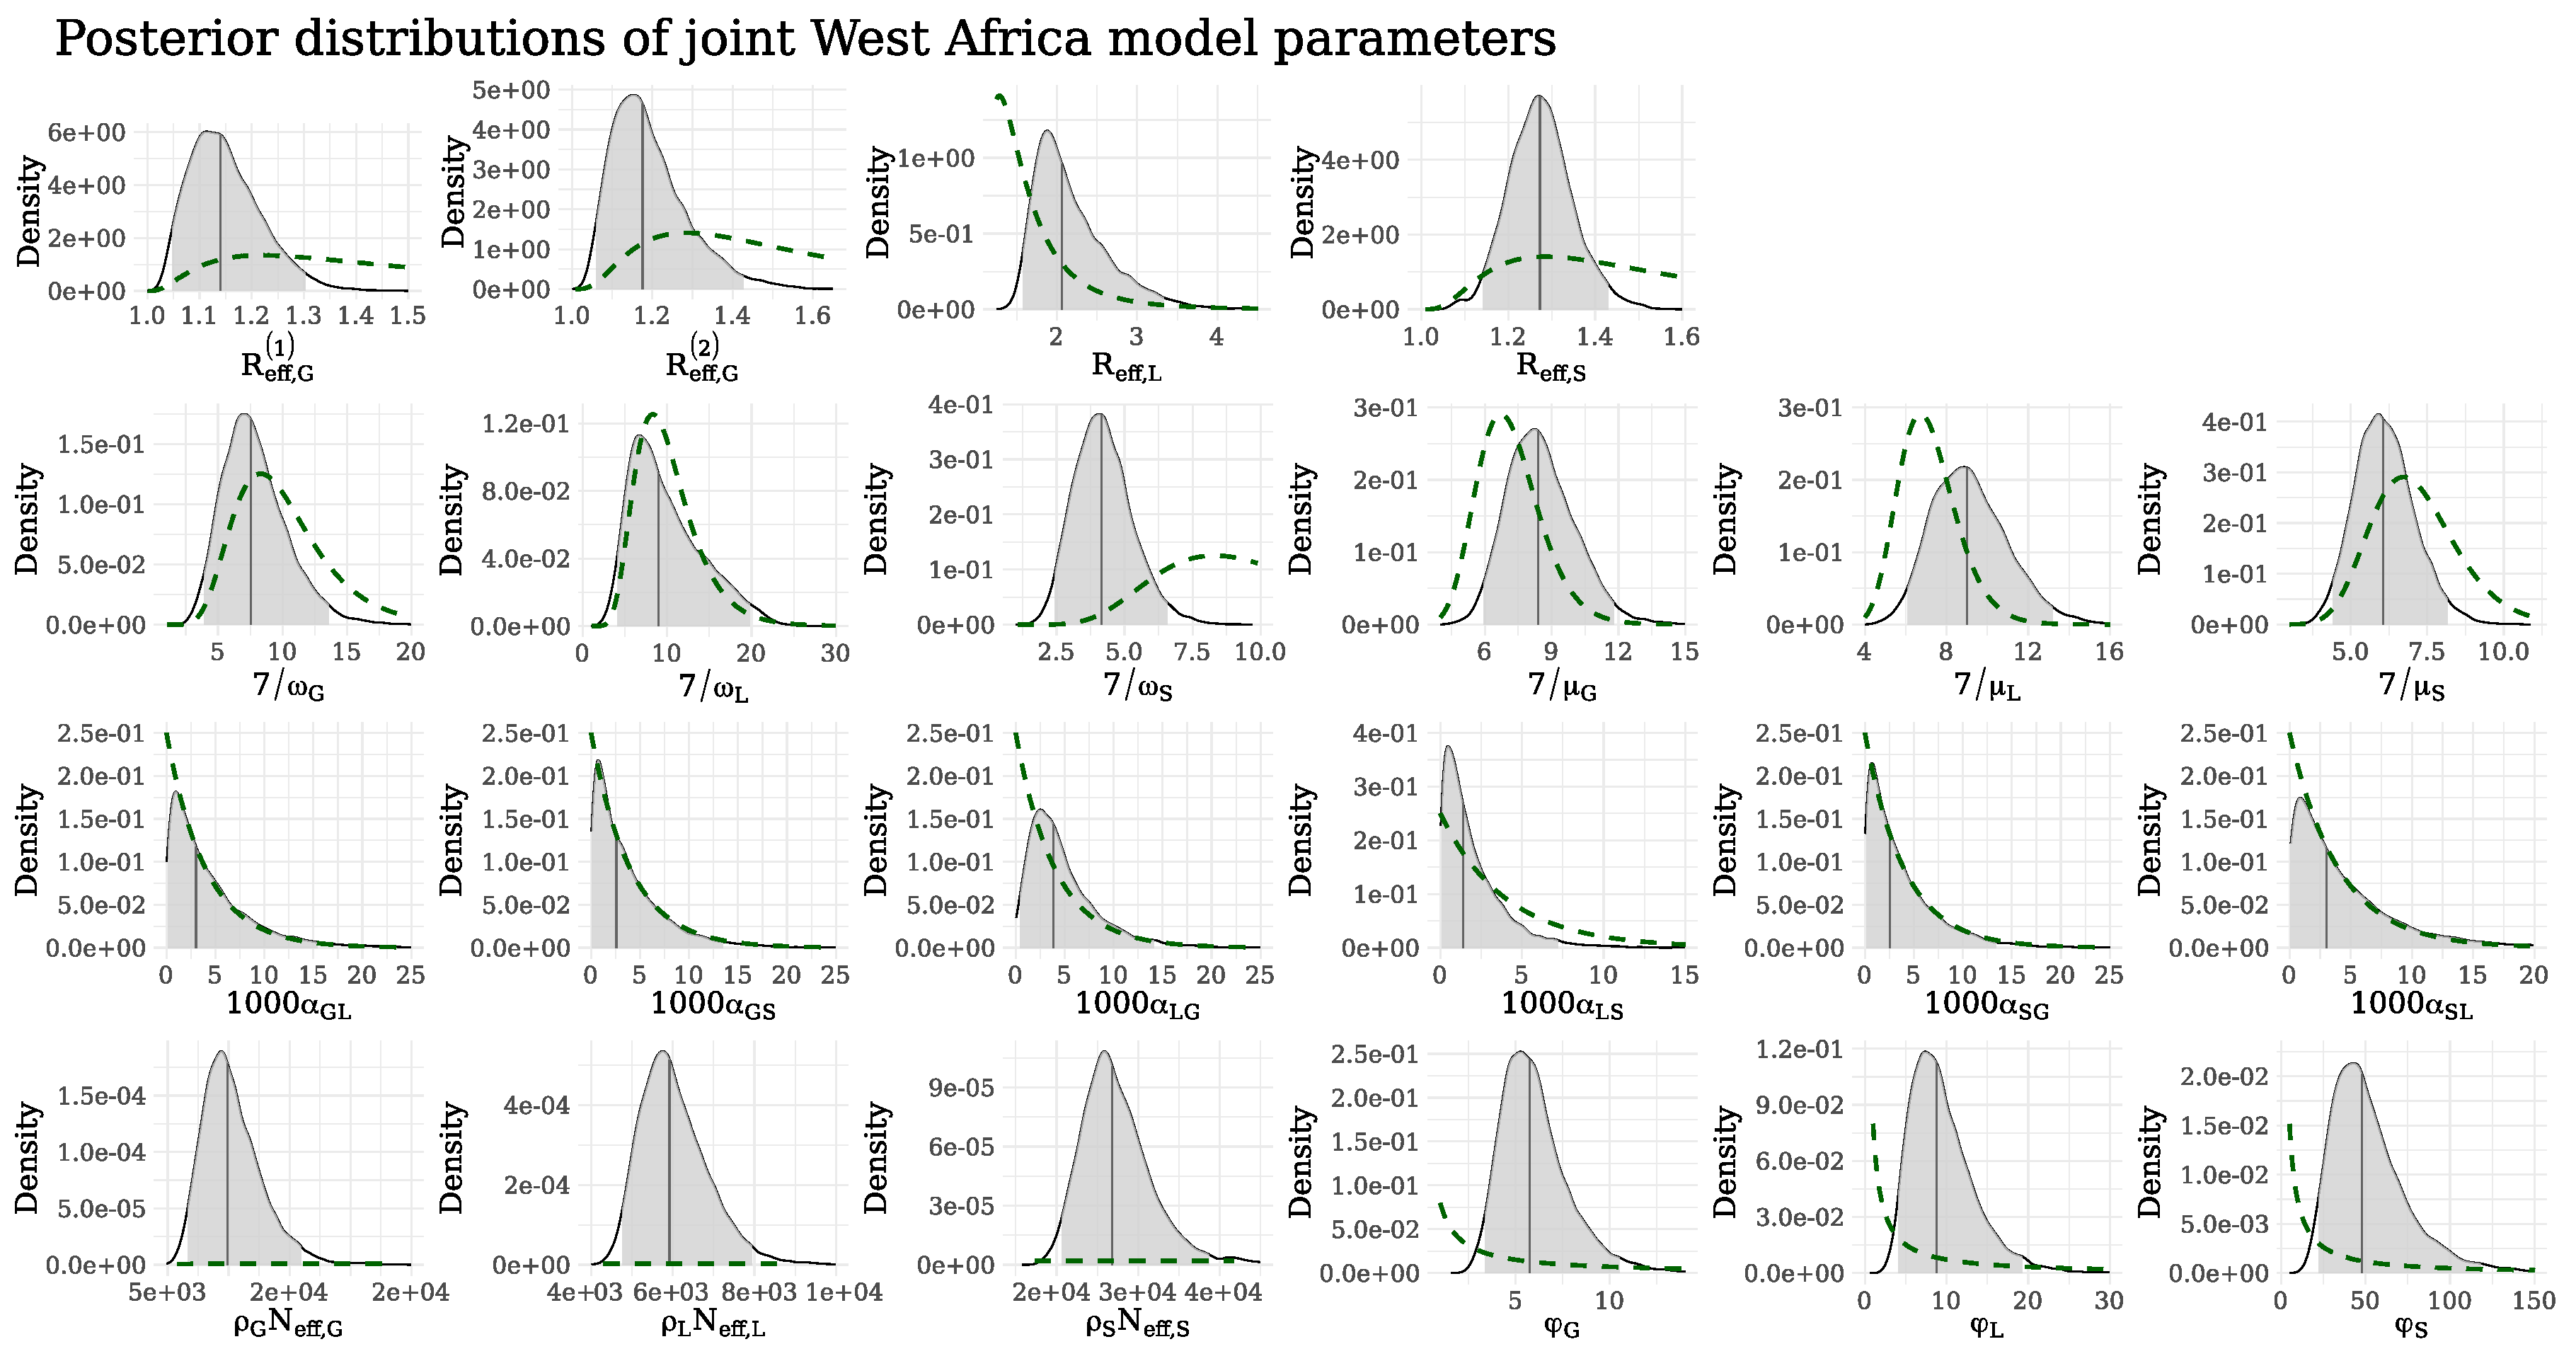
\includegraphics[width=\linewidth]{figures/ebola_joint_posts}
		\caption[Posterior distributions of parameters of the main stratified SEIR model fit to data from the West Africa Ebola outbreak.]{Posterior distributions of parameters of the main stratified SEIR model fit to data from the West Africa Ebola outbreak under tight priors. We show posterior medians (solid gray lines), 95\% Bayesian credible intervals (light gray areas under the posterior densities), prior densities (induced priors for the reporting rate and latent period durations) over the posterior ranges (dashed green curves). $ R_{eff} = \beta N_{eff}/\mu $ is the effective reproductive number, where $ \beta $ is the per--contact infection rate, $ N_{eff} $ is the effective population size, and $ \mu $ is the recovery rate. The latent and infectious period durations, $ 7/\omega $ and $ 7/\mu $, respectively, are given in days. The effective number of cross--border infectious contacts in country $ B $ per 1000 infected individuals in country $ A $ is $ 1000\alpha_{AB} $. The effective reporting rate is $ \rho N_{eff} $, and $ \phi $ is the negative binomial over--dispersion parameter. Subscripts indicate countries.}
		\label{fig:ebola_joint_posts}
	\end{fullpage}
\end{sidewaysfigure}

\begin{sidewaysfigure}[htbp]
	\centering
	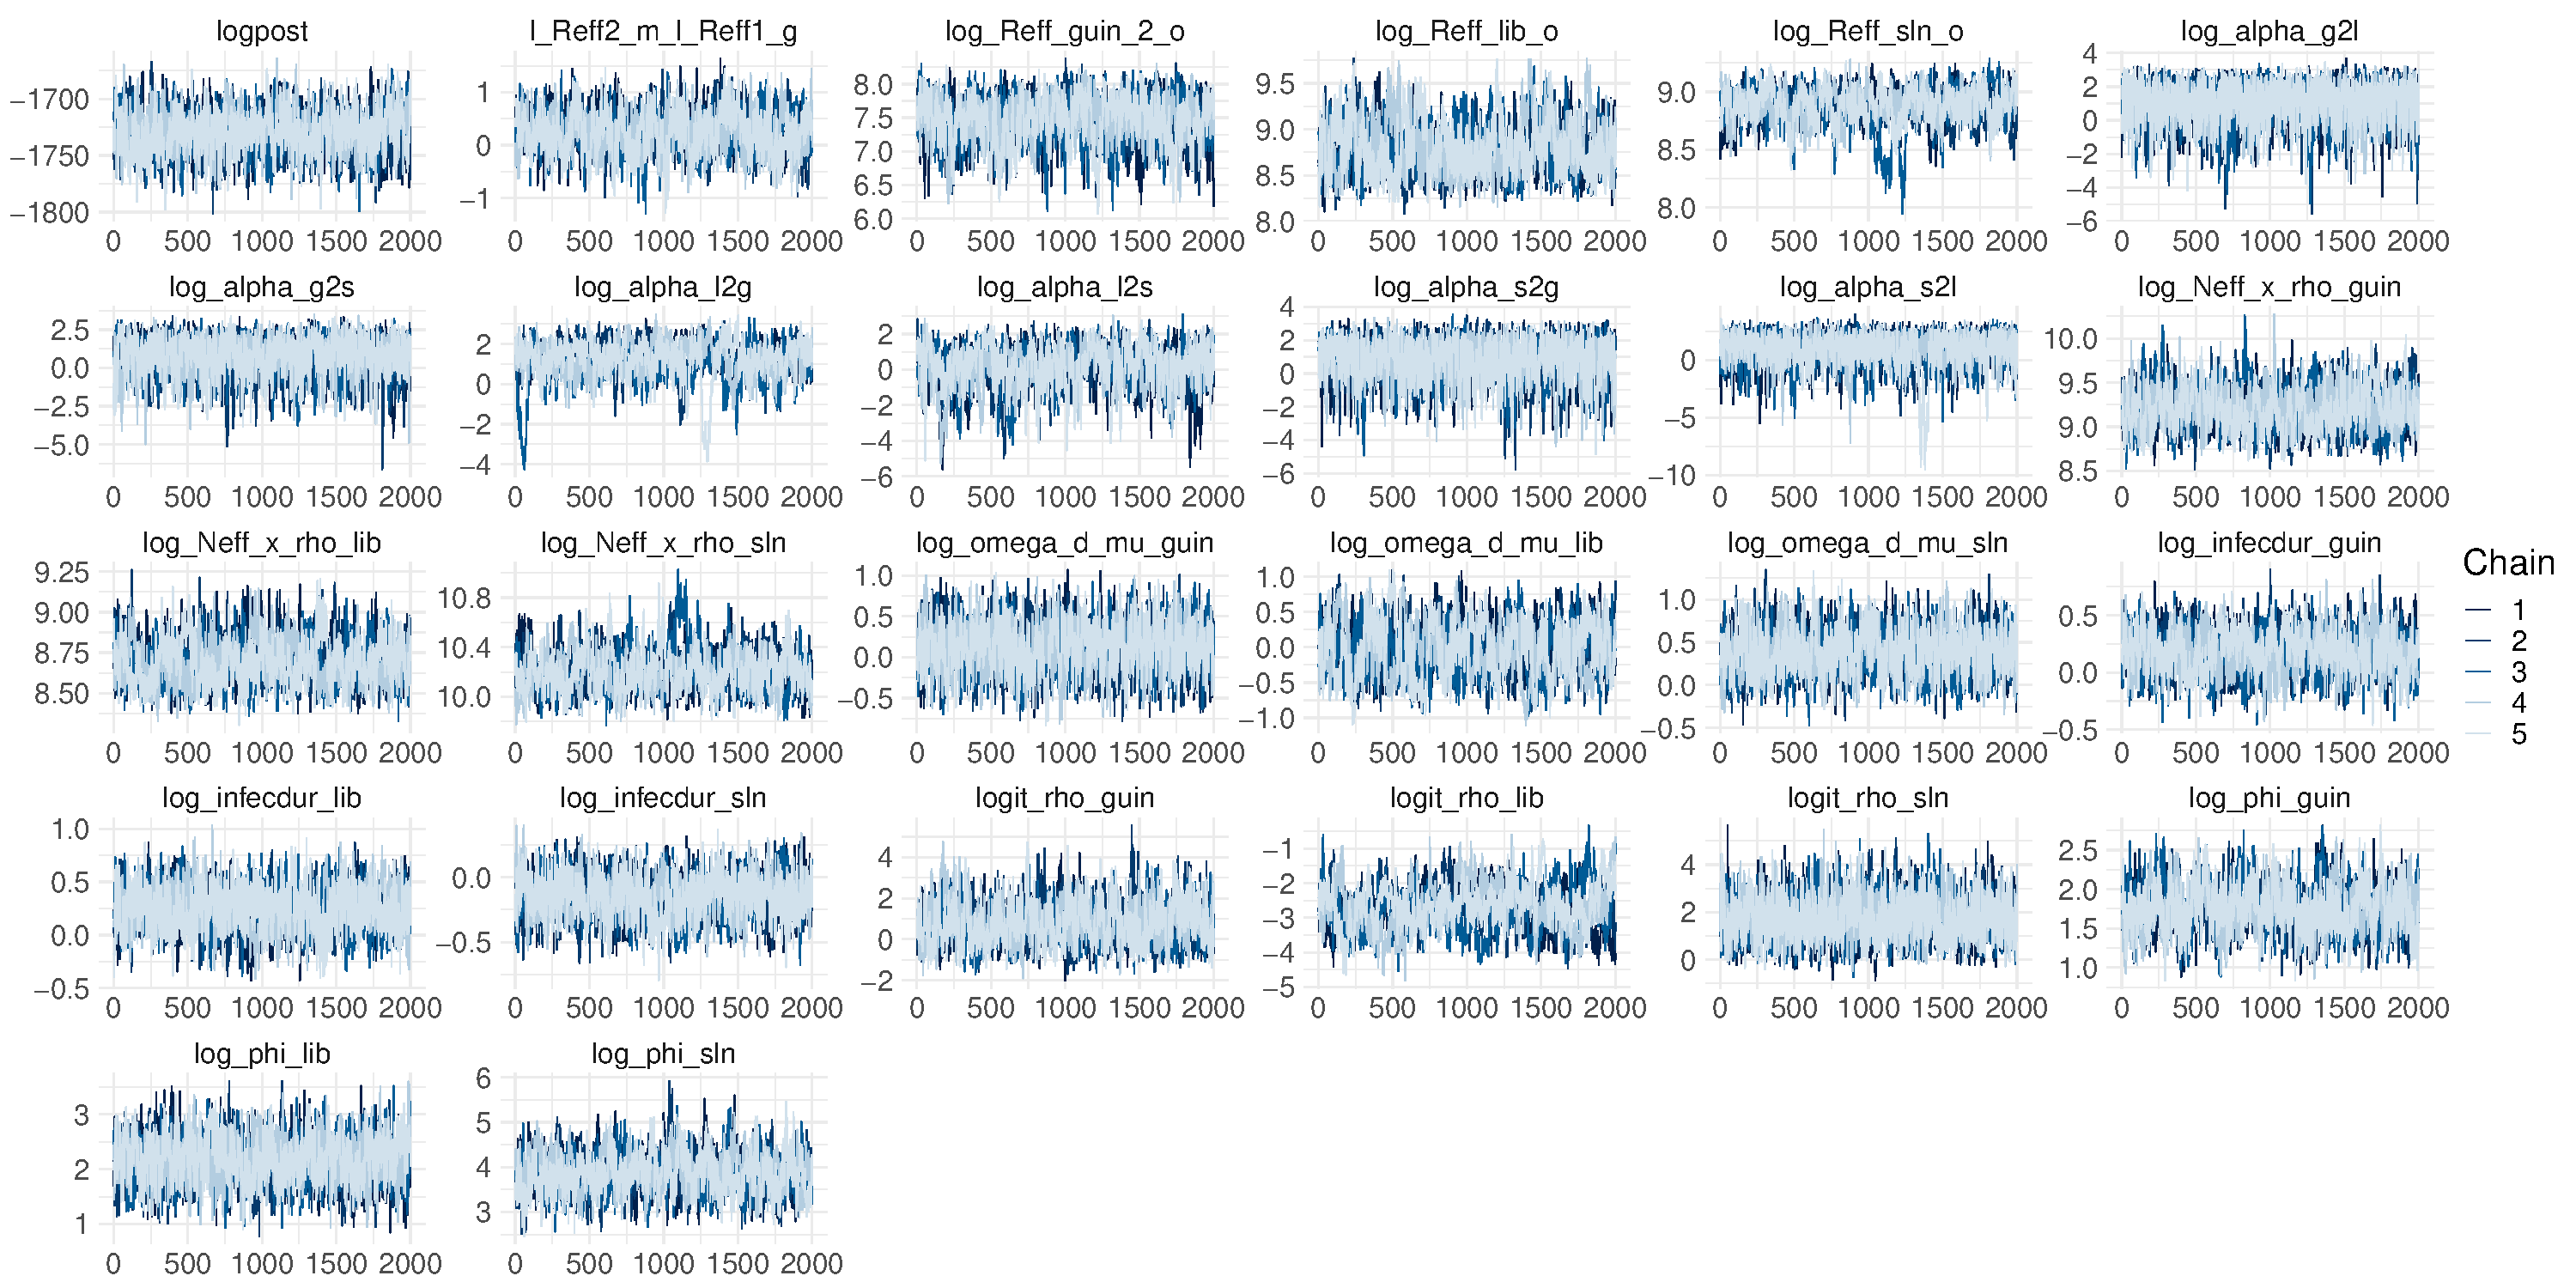
\includegraphics[width=\linewidth]{figures/ebola_joint_traces}
	\caption{Posterior traceplots for a stratified SEIR model fit to a simulated Ebola outbreak.}
	\label{fig:ebolajointtraces}
\end{sidewaysfigure}

\begin{figure}[htbp]
	\centering
	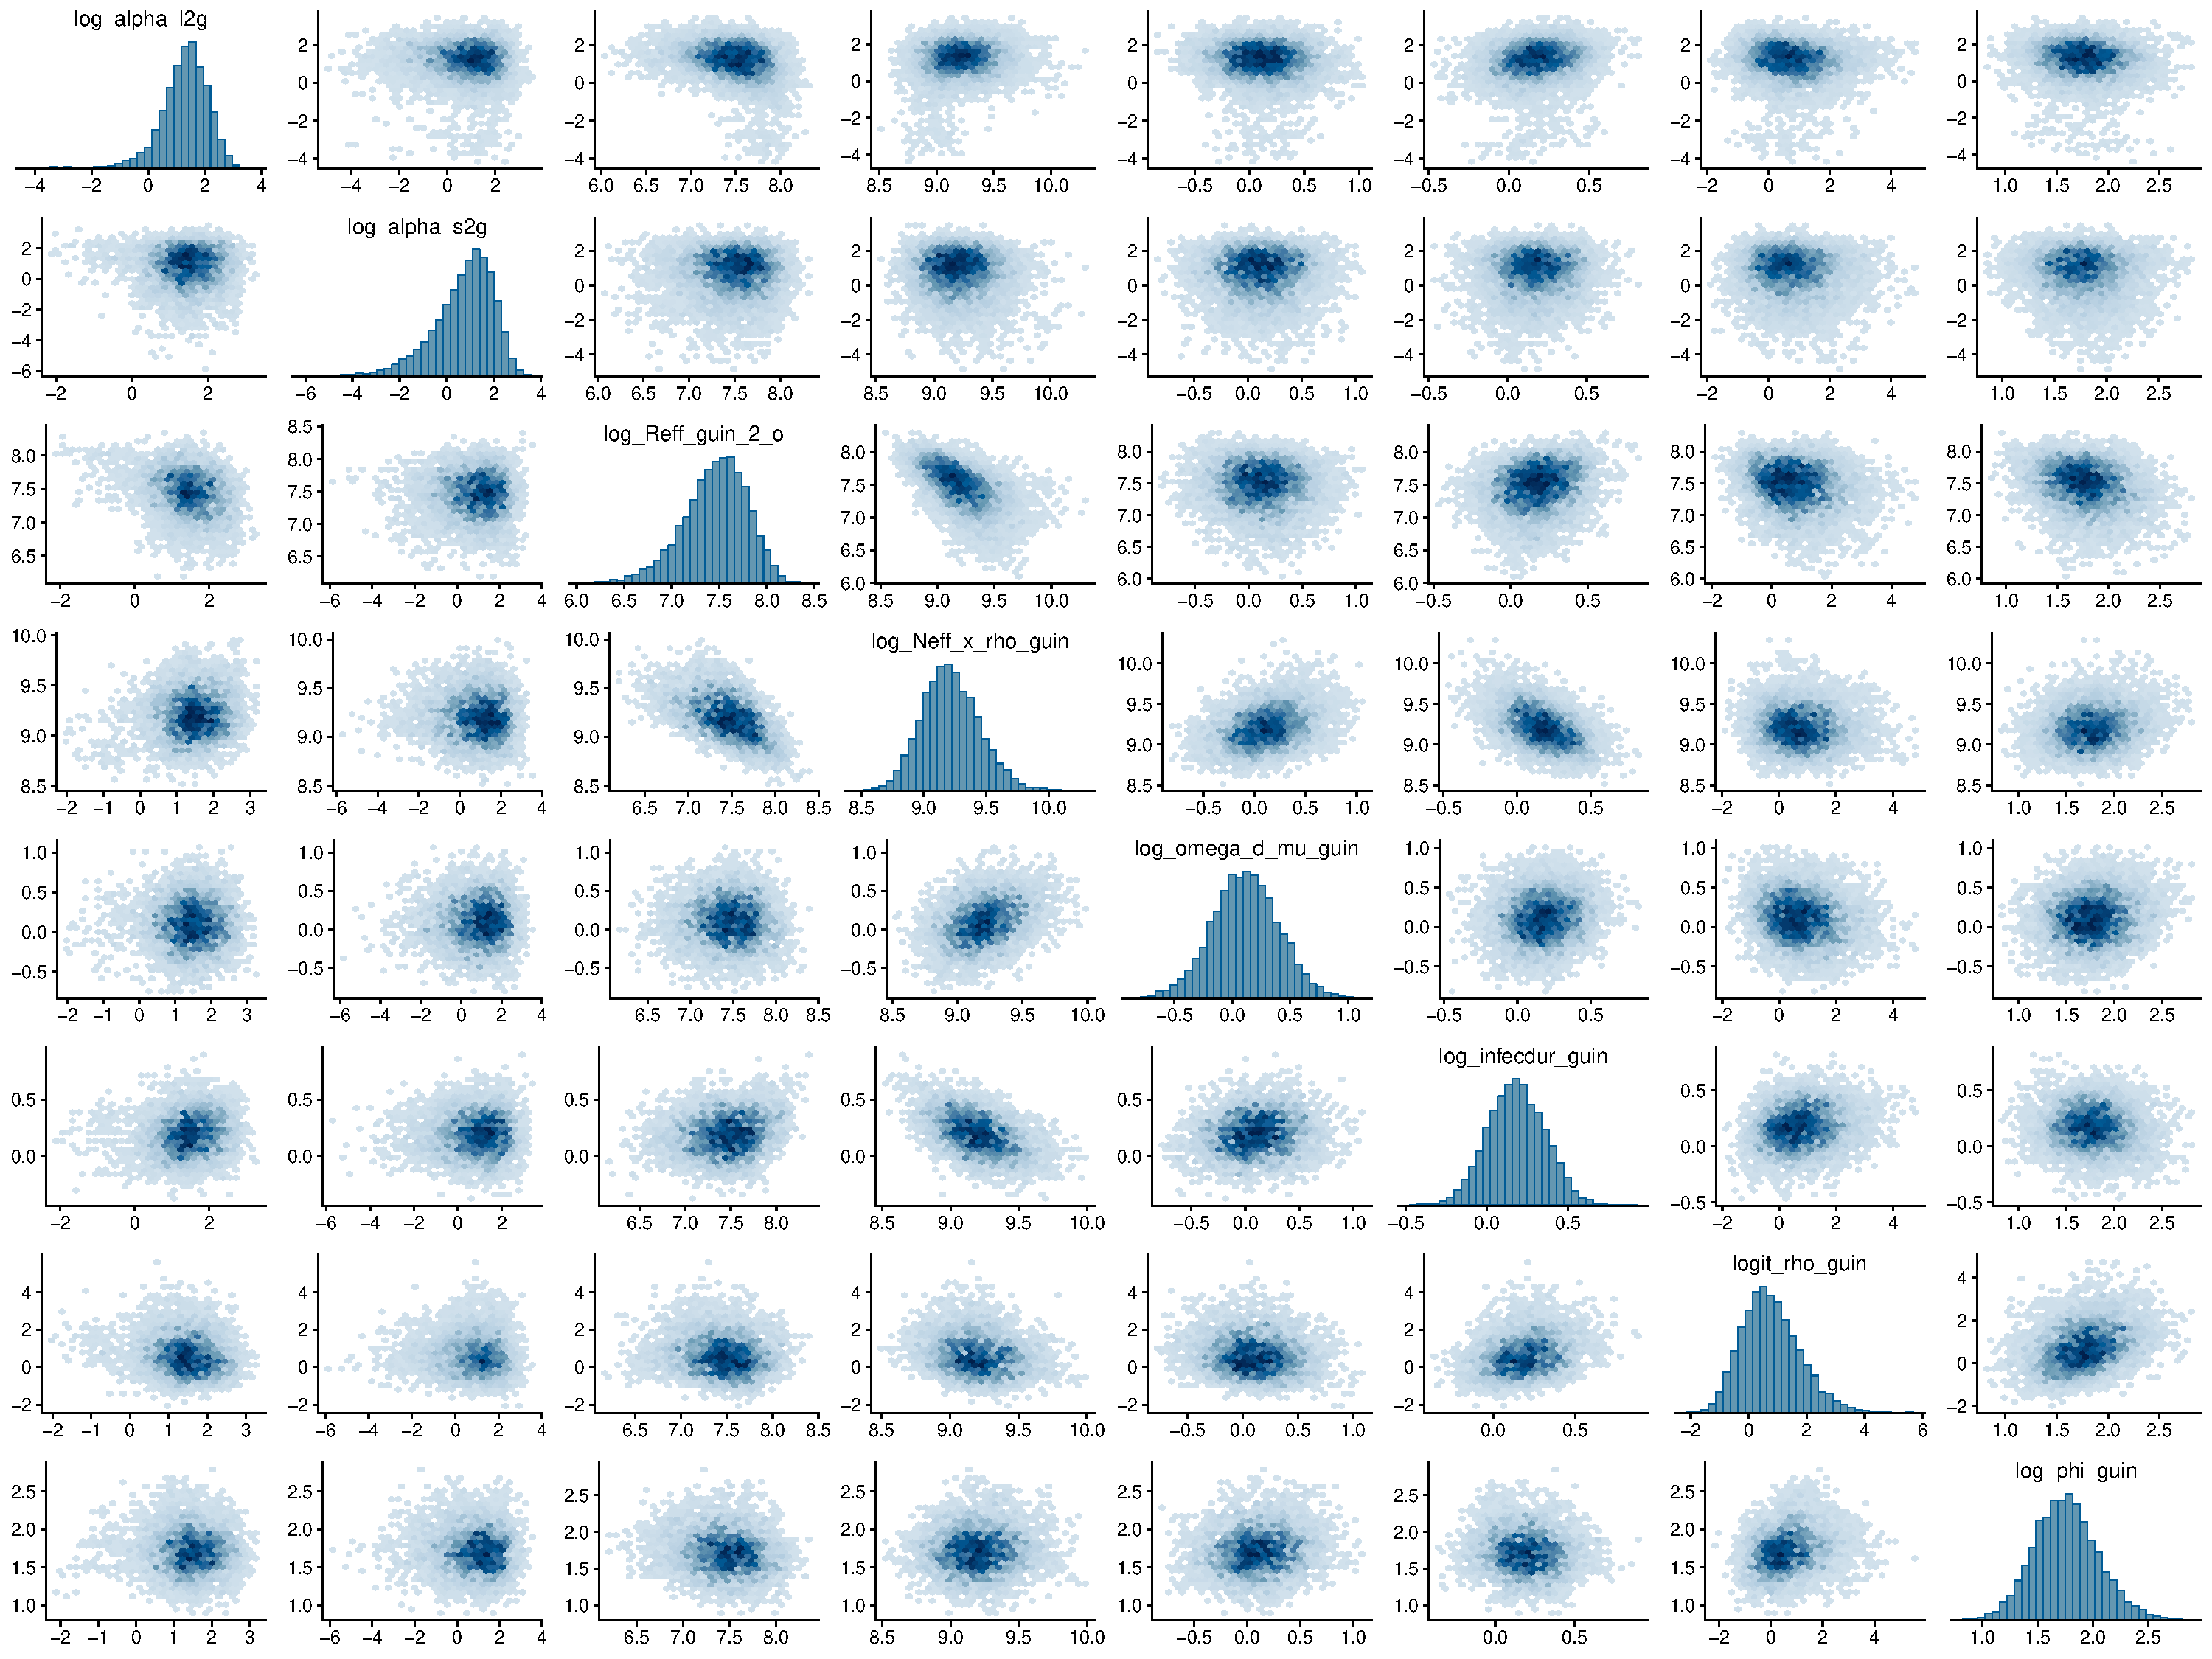
\includegraphics[width=\linewidth]{figures/ebola_joint_pairs_guin}
	\caption{Scatterplots of Guinea--specific parameters in a stratified SEIR model fit to data from the West Africa Ebola outbreak.}
\end{figure}

\begin{figure}[htbp]
	\centering
	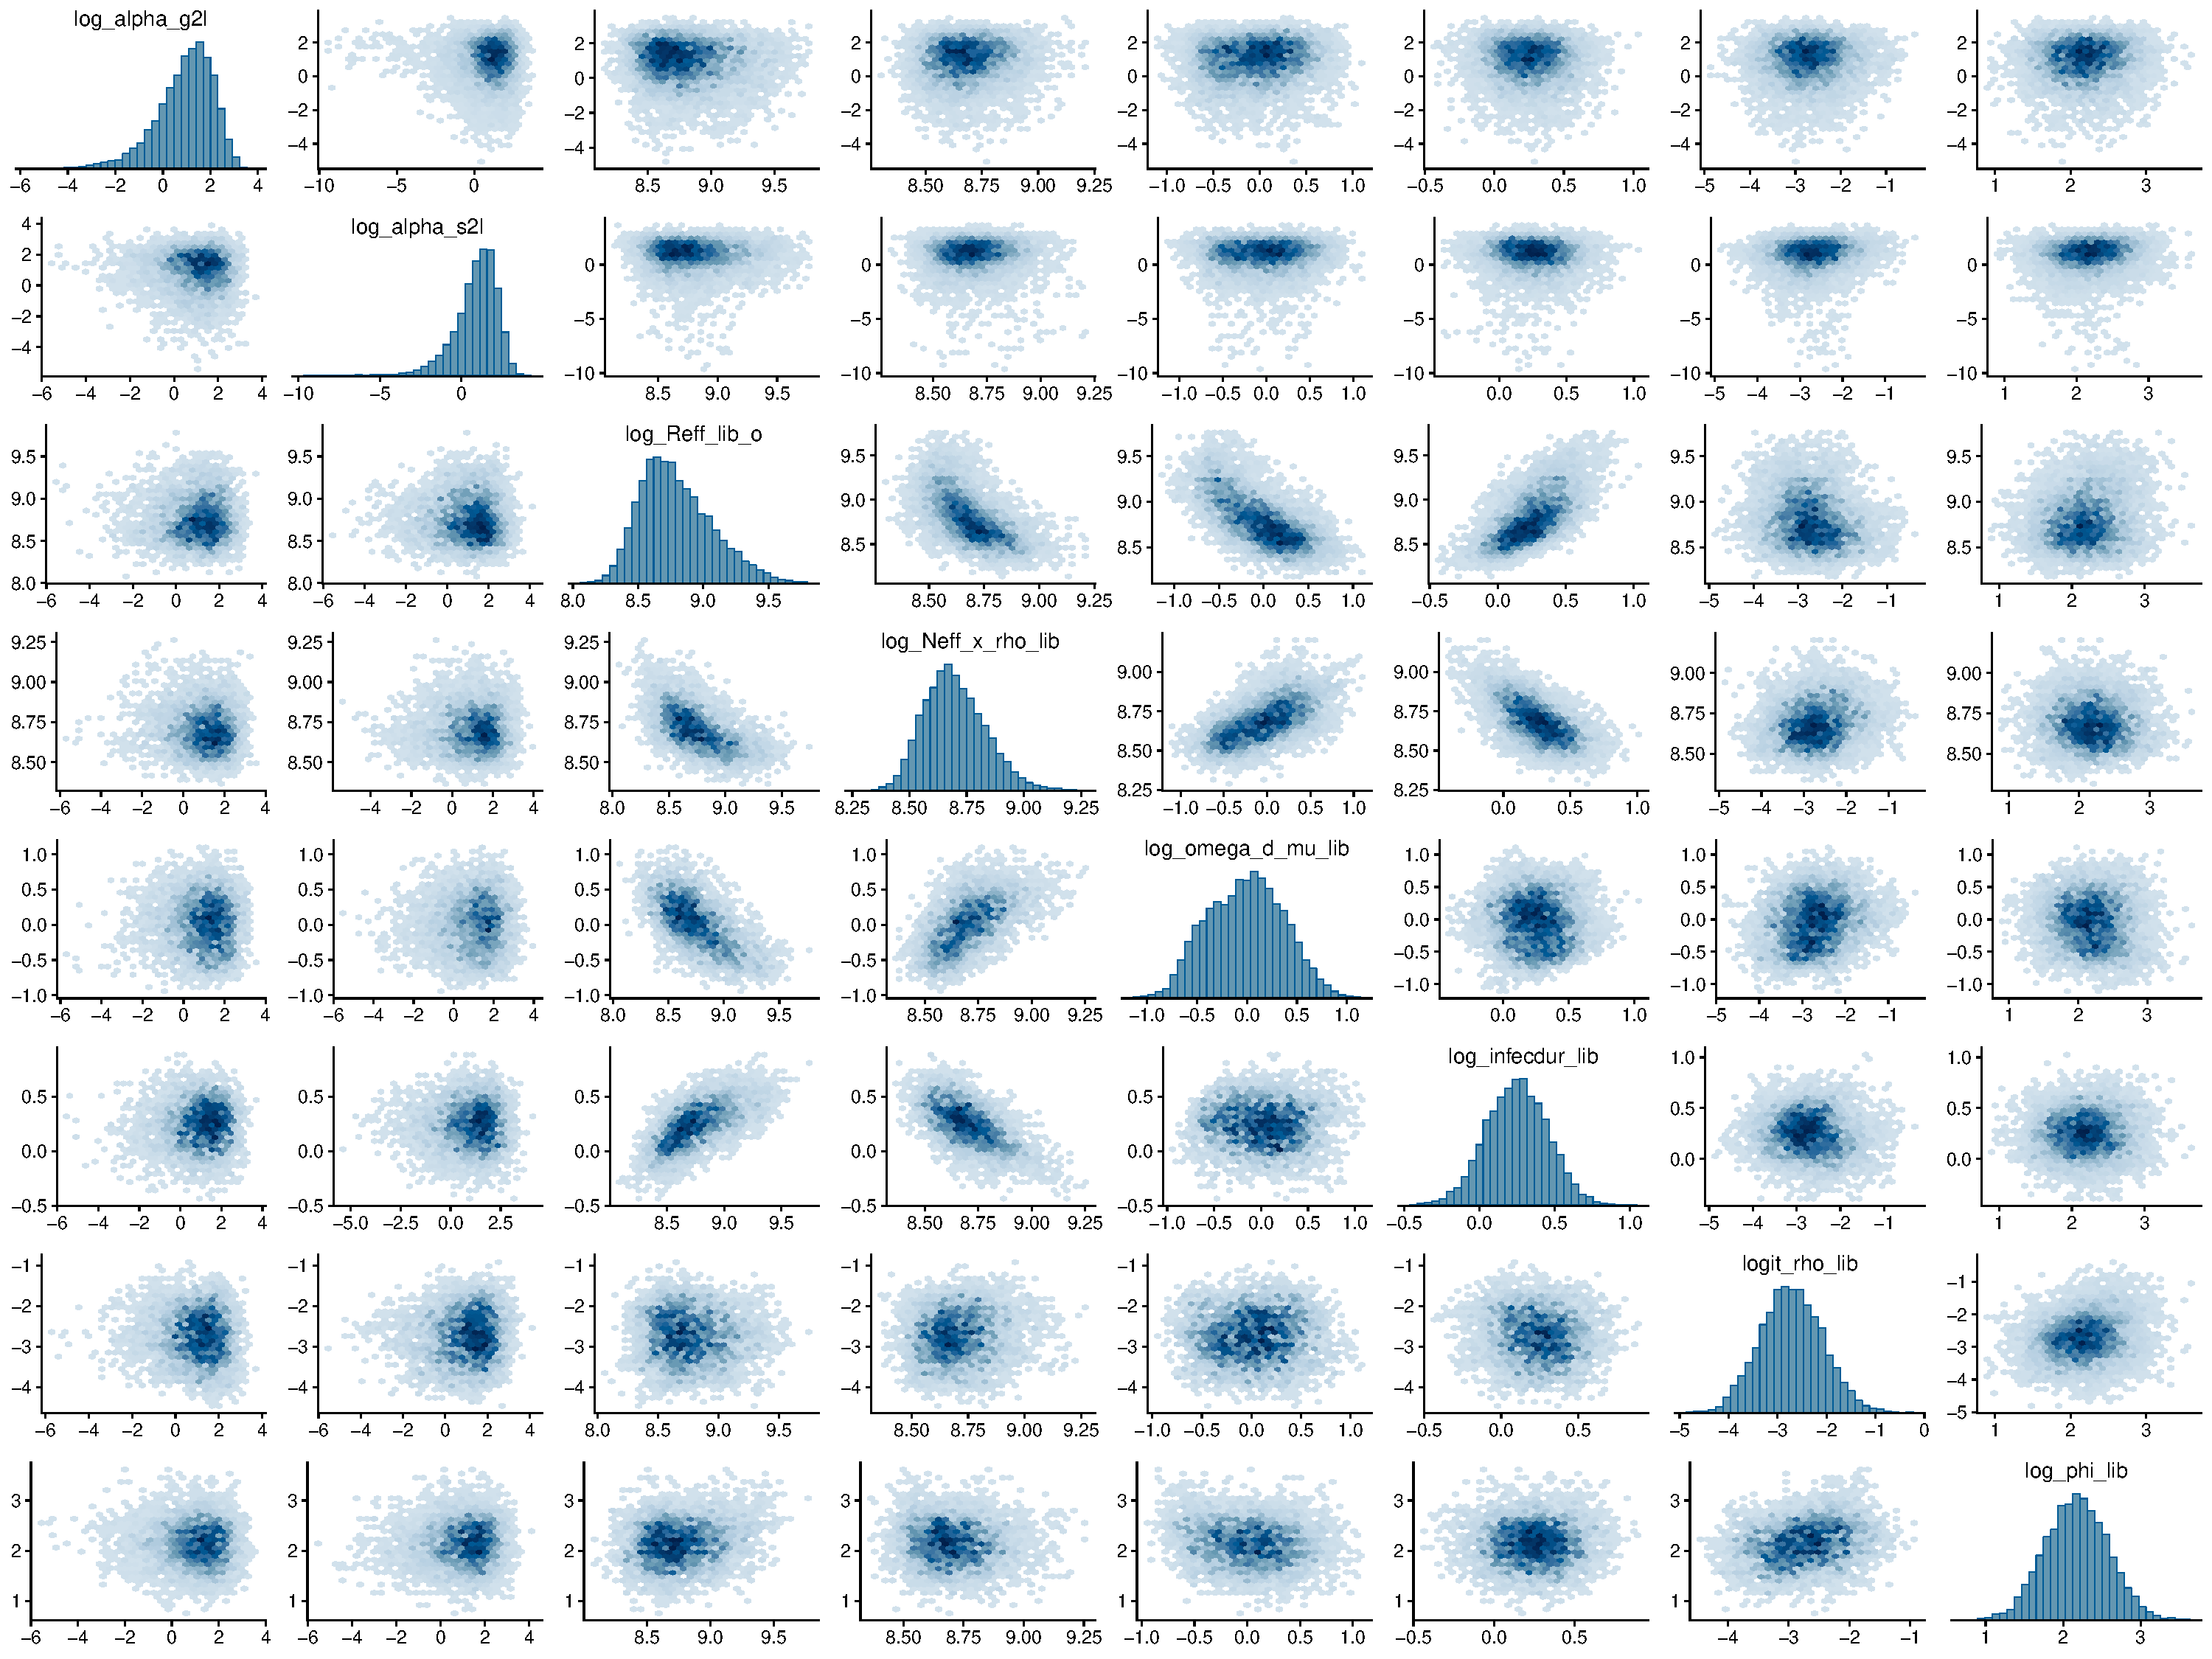
\includegraphics[width=\linewidth]{figures/ebola_joint_pairs_lib}
	\caption{Scatterplots of Liberia--specific parameters in a stratified SEIR model fit to data from the West Africa Ebola outbreak.}
\end{figure}

\begin{figure}[htbp]
	\centering
	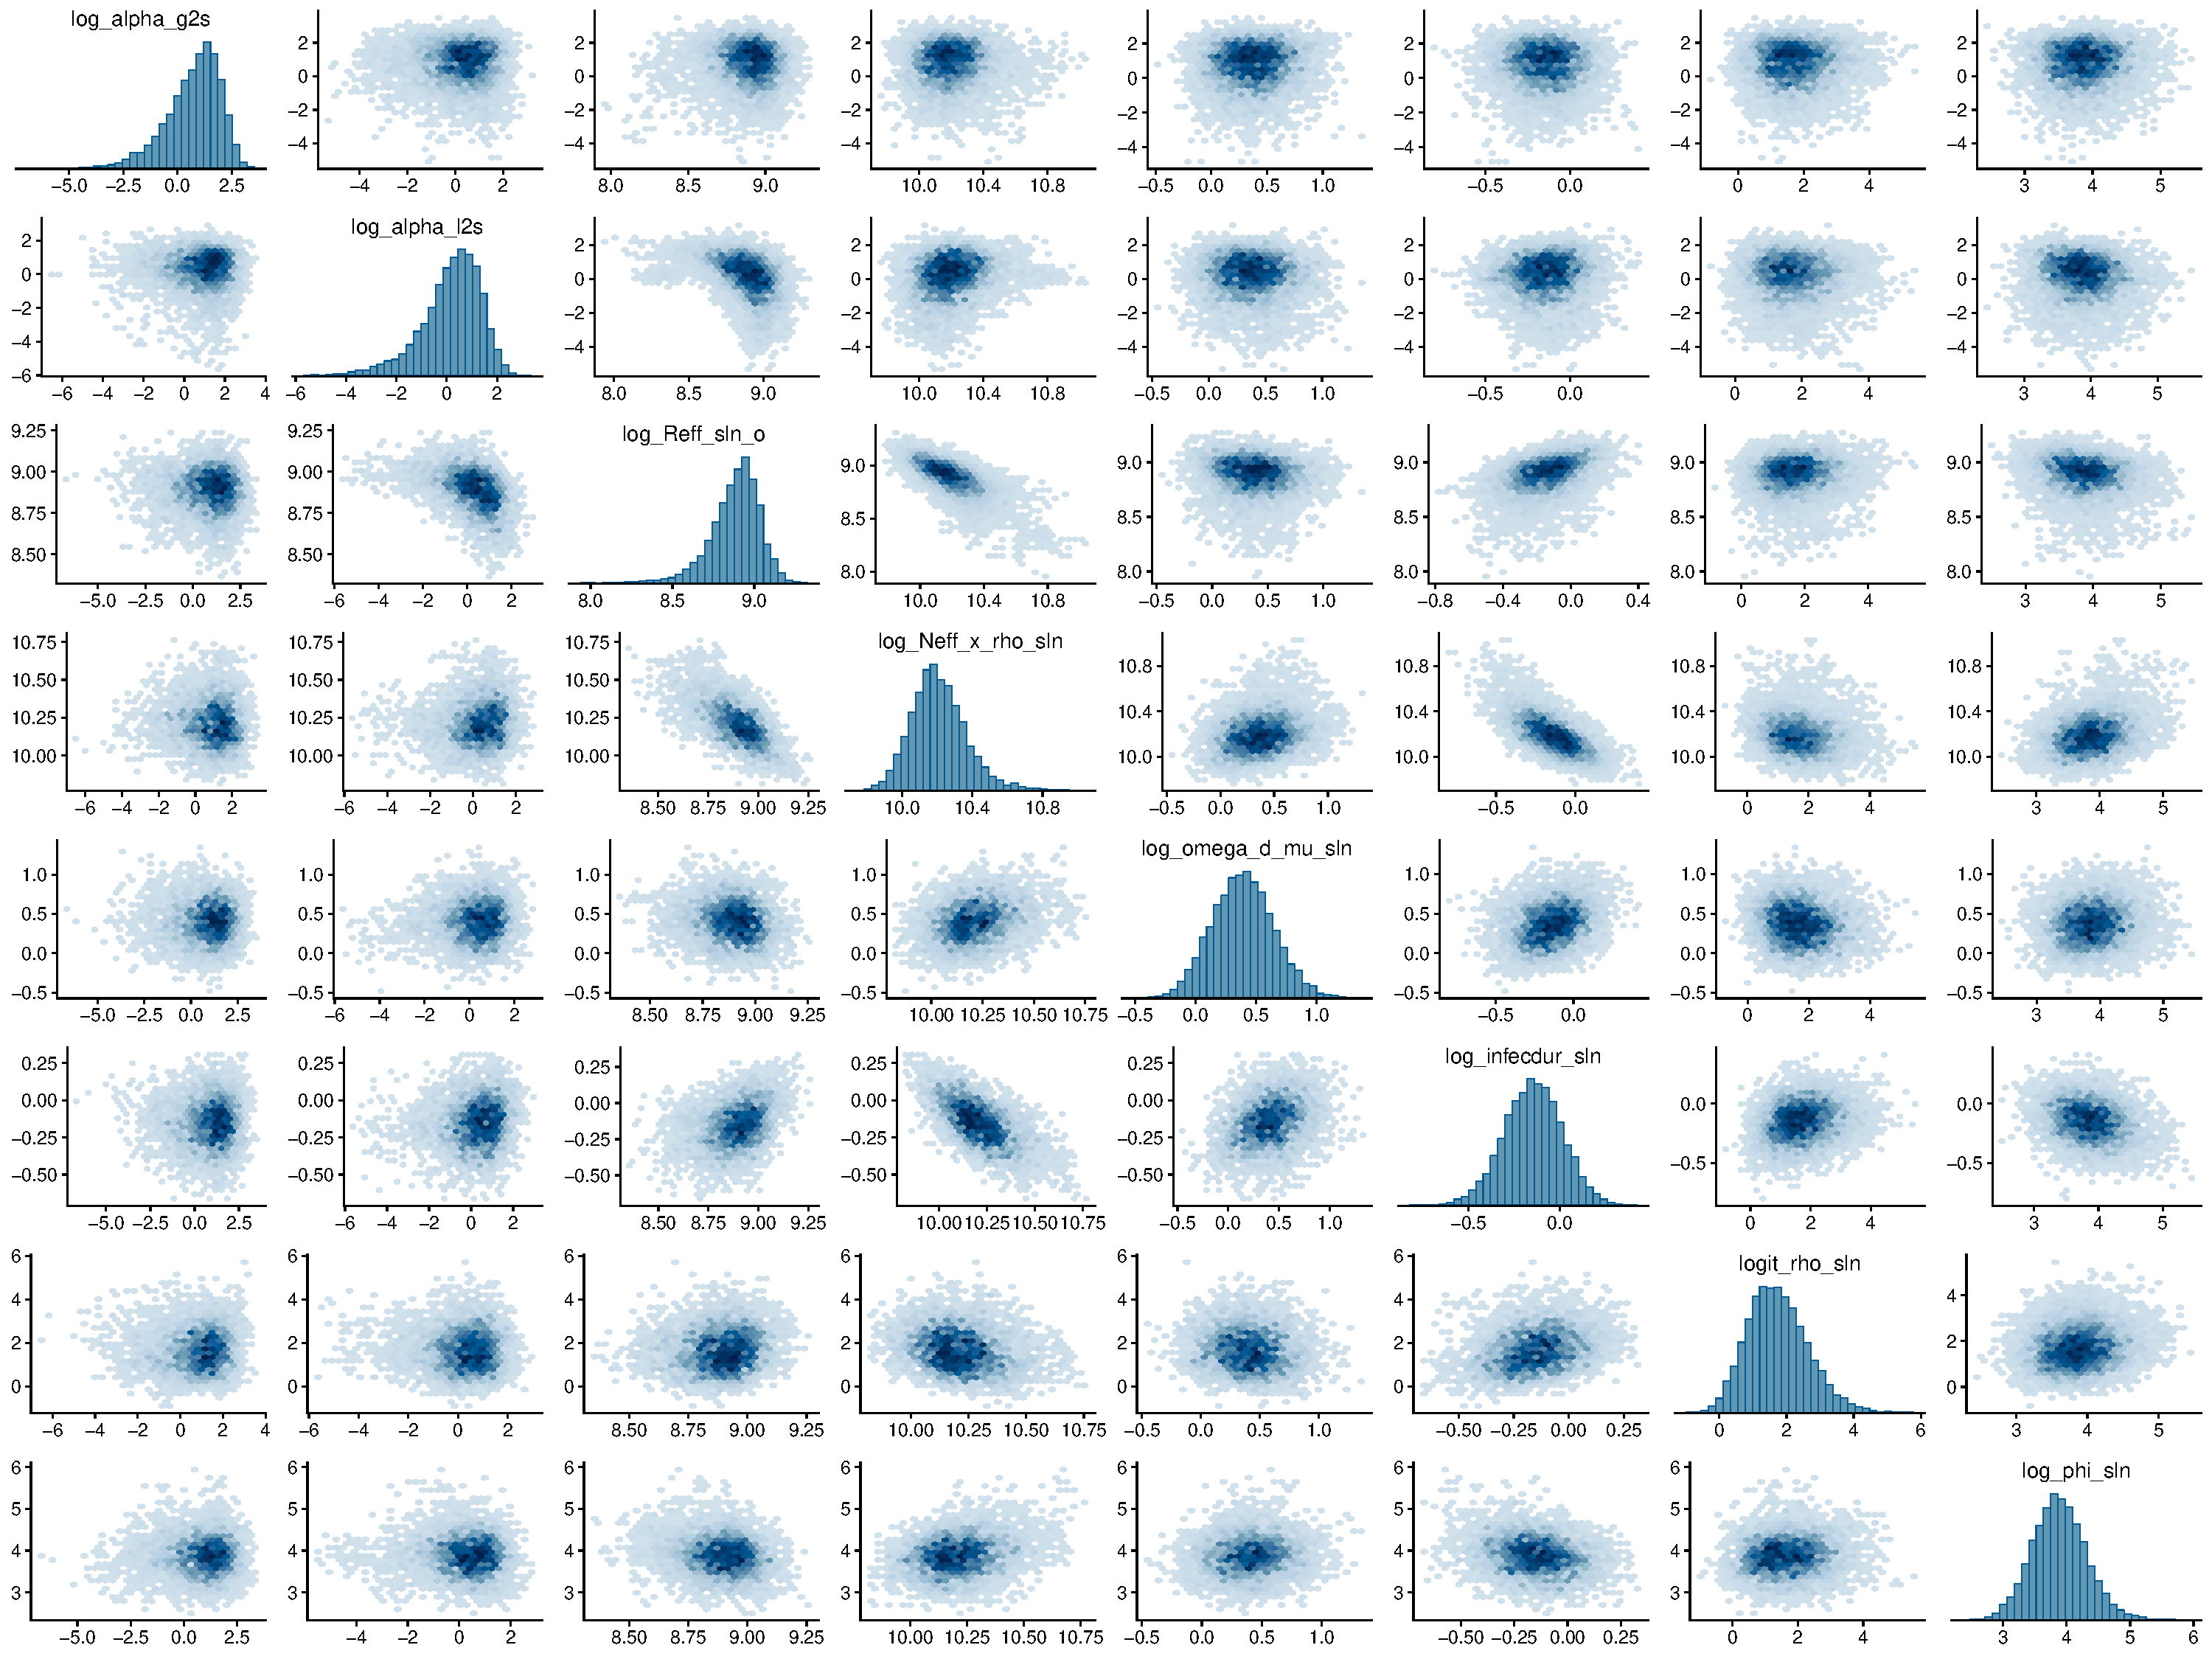
\includegraphics[width=\linewidth]{figures/ebola_joint_pairs_sln}
	\caption{Scatterplots of Sierra Leone--specific parameters in a stratified SEIR model fit to data from the West Africa Ebola outbreak.}
\end{figure}

\begin{figure}[htbp]
	\begin{fullpage}
		\centering
		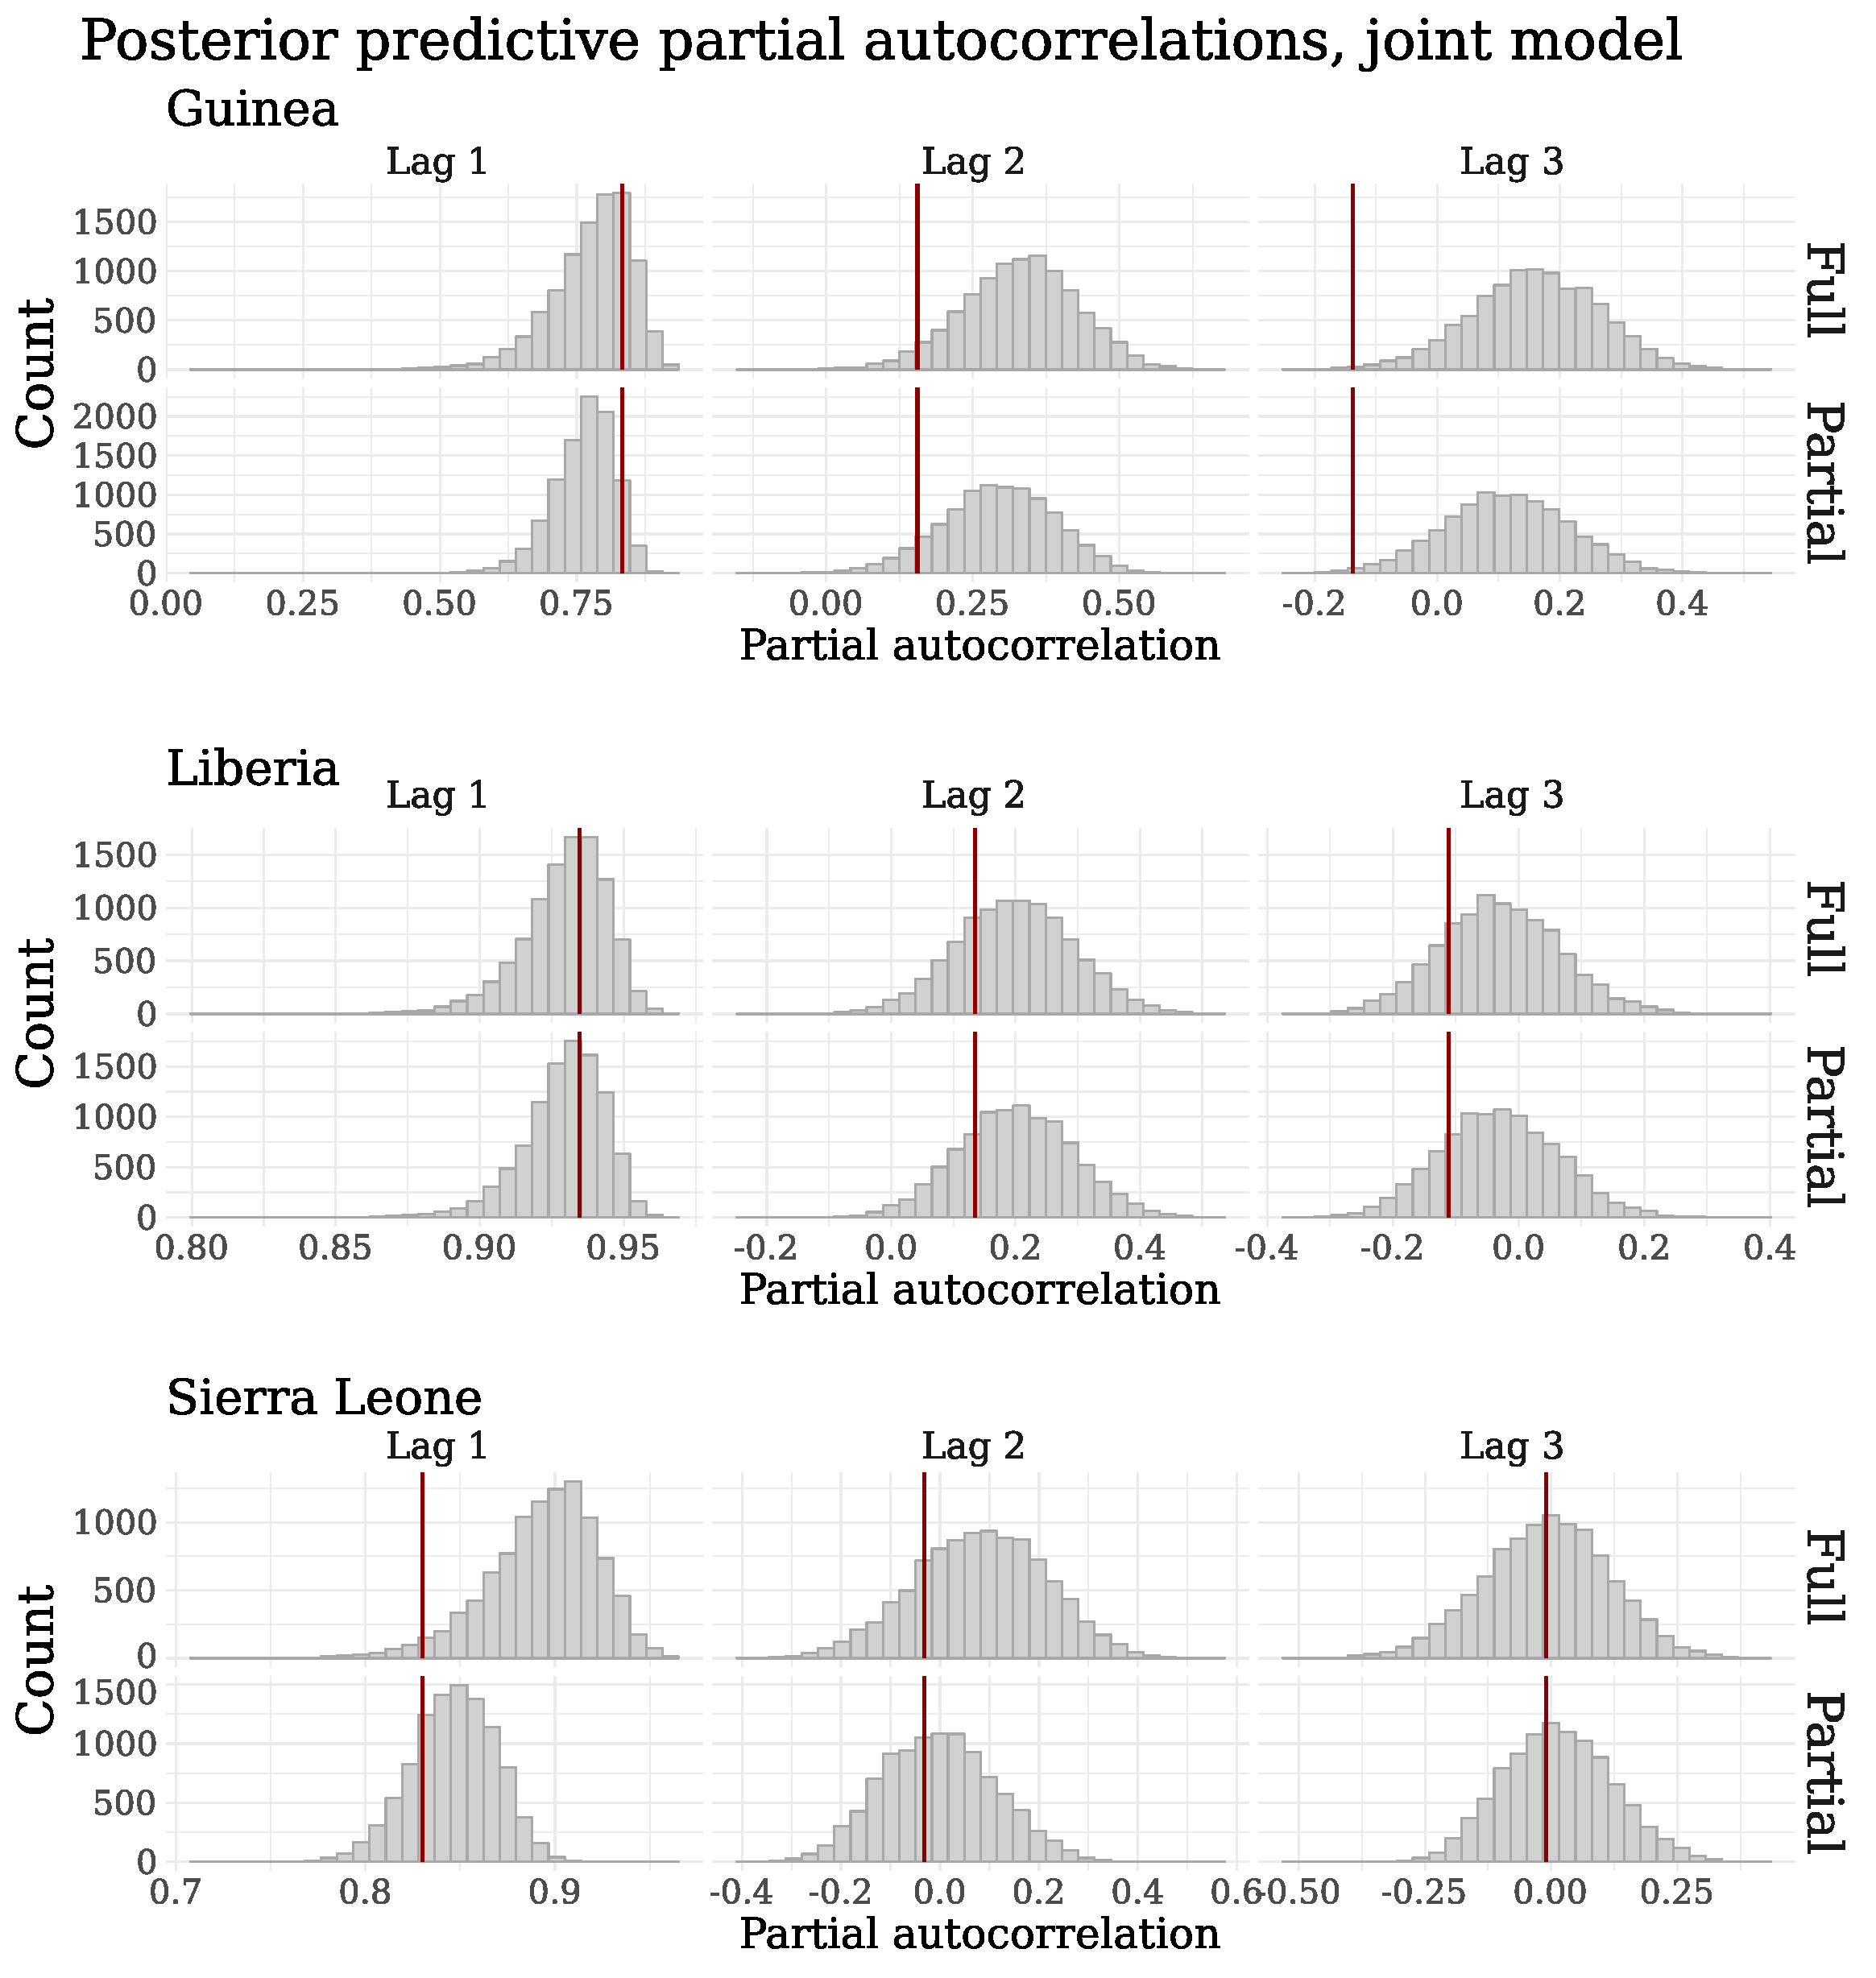
\includegraphics[width=0.8\linewidth]{figures/ebola_joint_pacfs}
		\caption[Posterior predictive distributions of partial autocorrelations for a stratified SEIR model fit to data from the West Africa Ebola outbreak.]{Distributions of partial autocorrelations at lags 1, 2, and 3 for datasets generated under the full and partial posterior predictive distributions for the main stratified SEIR model fit to data from the West Africa Ebola outbreak. Vertical red lines are the partial autocorrelations for the observed incidence data at the respective lags.}
		\label{fig:ebola_joint_pacfs}
	\end{fullpage}
\end{figure}

\begin{sidewaysfigure}[htbp]
	\begin{fullpage}
		\centering
		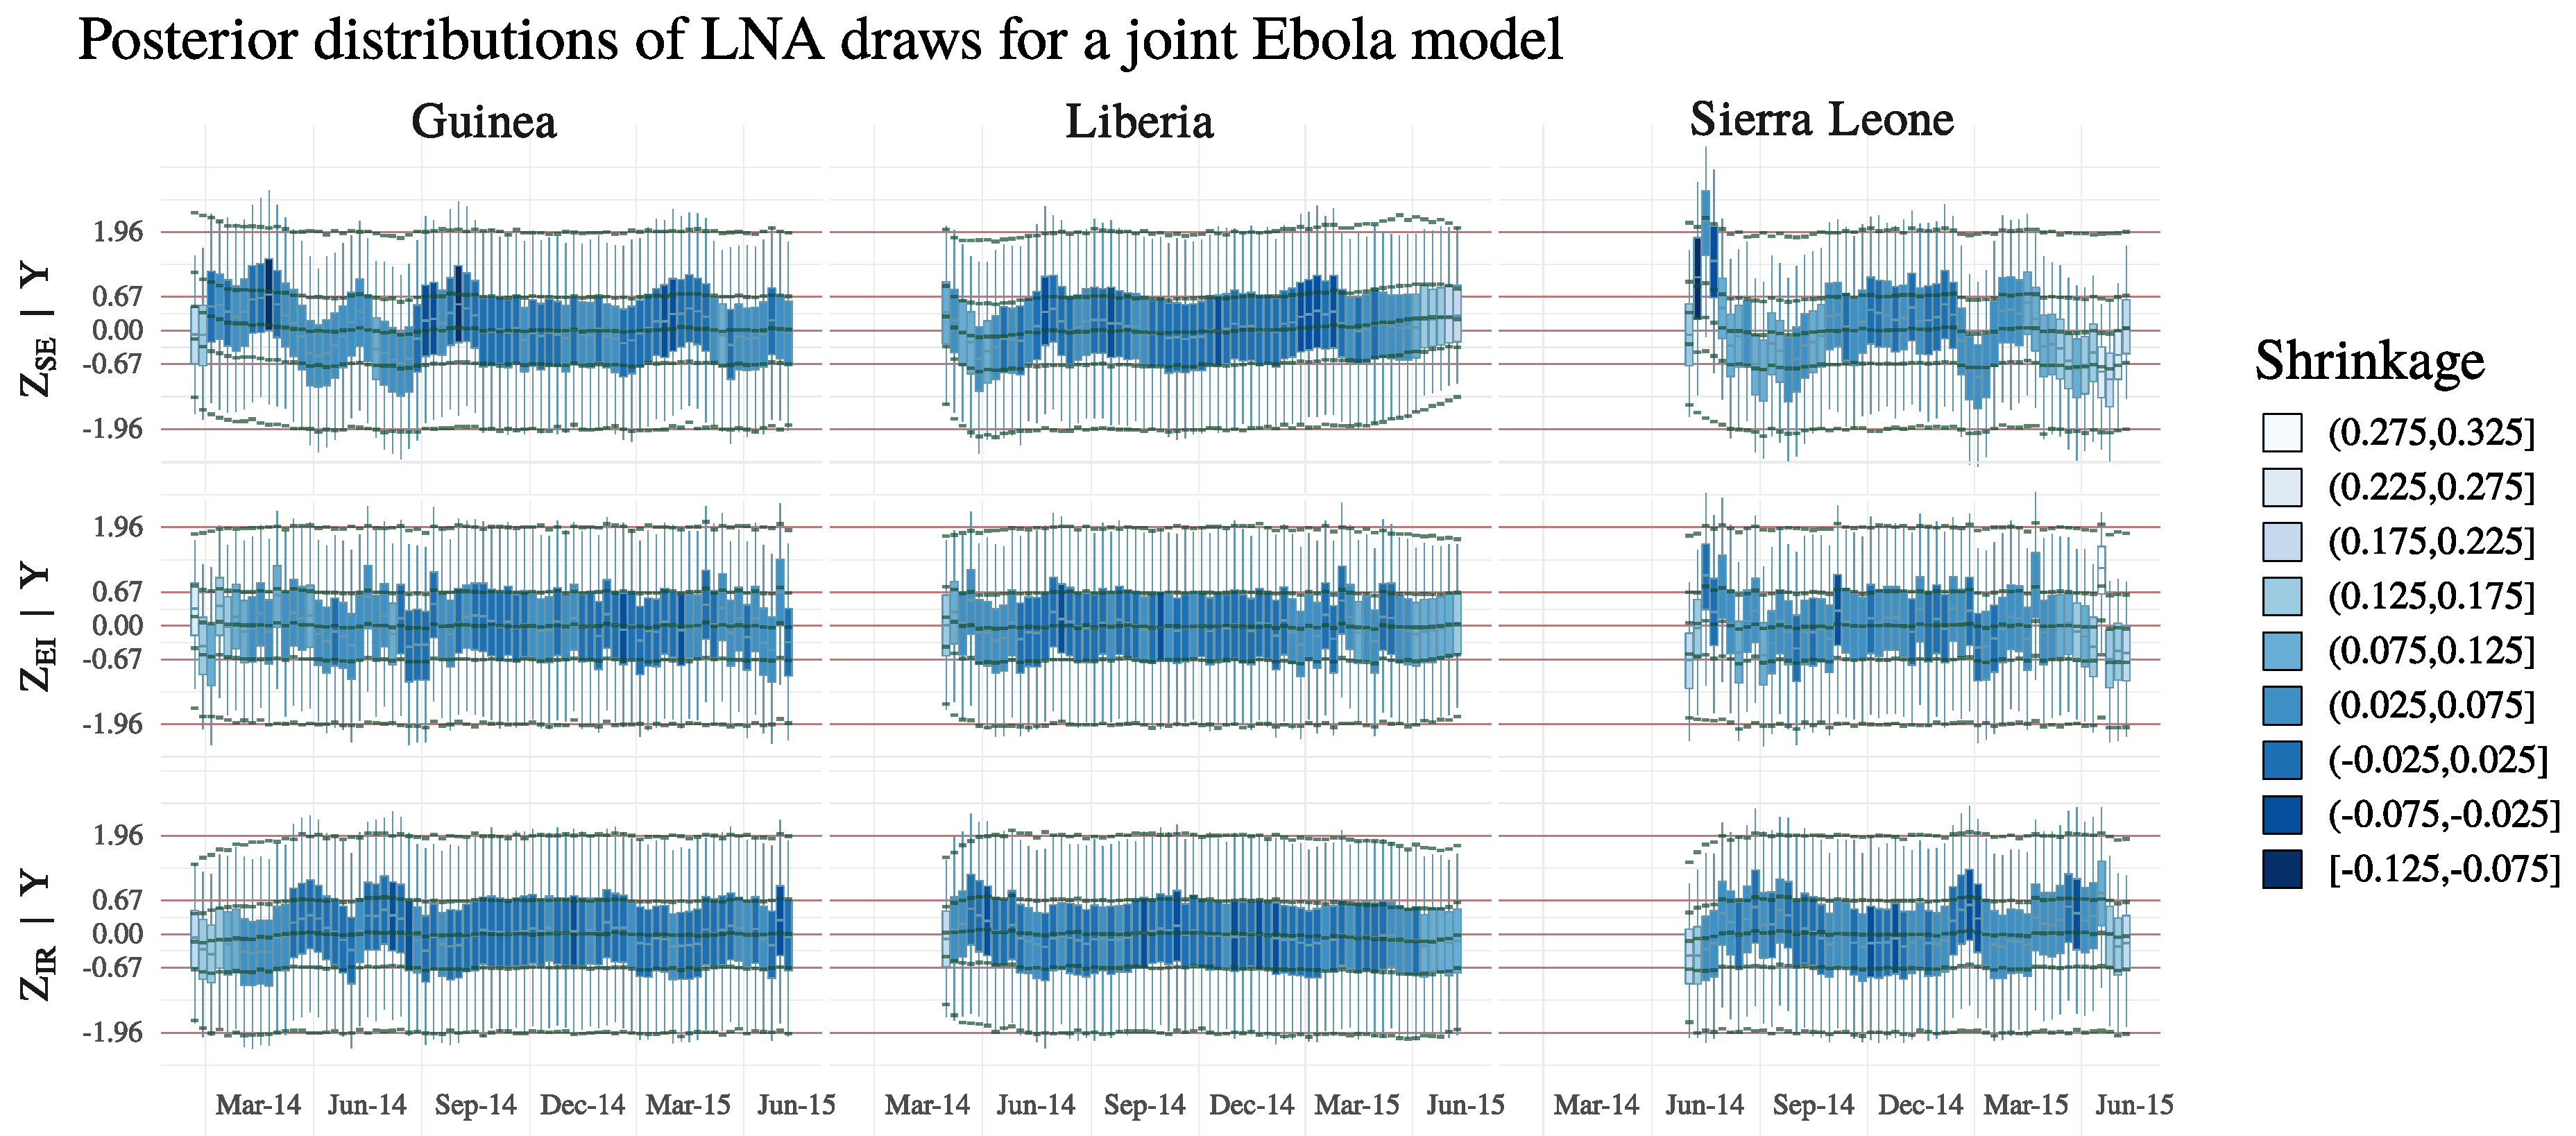
\includegraphics[width=\linewidth]{figures/ebola_joint_drawplots}
		\caption[Posterior distributions of LNA draws for the main stratified SEIR model fit to data from the West Africa Ebola outbreak.]{Posterior distributions of the LNA draws for exposures, infections, and recoveries (blue boxplots) in the main stratified SEIR model fit data from the Ebola outbreak in Guinea, Liberia, and Sierra Leone. The lower and upper whisker tips correspond to the $ 2.5^\mr{th} $ and $ 97.5^\mr{th} $ posterior quantiles, the lower and upper hinges to the $ 25^\mr{th} $ and $ 75^\mr{th} $ quantiles, and the middle hash mark to the posterior median. The solid red lines are the theoretical quantiles of the posterior predictive distribution (or equivalently, the prior distribution) of the LNA draws, drawn at the quantiles of a standard normal distribution corresponding to the boxplot quantiles. The green ticks are the estimated quantiles of the posterior predictive distributions of the LNA draws, accounting for boundary conditions on the state space of the latent process and obtained by simulating LNA paths from the posterior predictive distribution. The posterior distributions of LNA draws are shaded according to the level of posterior shrinkage, computed as one minus the ratio of standard deviations of LNA draws in the posterior and prior.}
		\label{fig:ebola_joint_drawplots}
	\end{fullpage}
\end{sidewaysfigure}

\newpage
\section{LNA Implementation Details and LNA Model Vignettes}
\label{sec:lna_implementation_vignettes}